\chapter{Analiza wyników badań}\label{Chapter_AnalizaRezultatow}

  \section{Specyfikacja przeprowadzonych badań}\label{Section_SpecyfikacjaPrzeprowadzonychBadan}

    \subsection{Definicje gestów}\label{Subsection_DefinicjeGestow}

      W~ramach przeprowadzonych badań stworzono definicje poszczególnych gestów wykonywanych dłońmi użytkownika. Poniższa specyfikacja ma na celu uwspólnienie pojęć potrzebnych przy przeprowadzeniu analizy jakościowej oraz wydajnościowej.

      Wytyczne były pomocne przy procesie akwizycji oraz obróbki danych wejściowych. Wszystkie stworzone materiały testowe są zgodne z~przedstawionymi protokołami. W~zbiorze danych wejściowych można wyróżnić następujące definicje gestów:

        \gest{Zgniatanie}
             {Gest wykonywany na jednolitej i~gładkiej powierzchni.}
             {Zaciśnięcie dłoni od rozwarcia do pięści.}
             {Prawa dłoń.}
             {W~pozycji wejściowej otwarta dłoń, w~pozycji końcowej pięść zwrócona palcami do kamery, z~kciukiem na wierzchu.}
             {Gest powinien być wykonywany bez poruszania dłonią, z~jednolitą prędkością.}
             {Otwarta dłoń z~rozłożonymi palcami, skierowana wewnętrzną stroną do kamery.}
             {Punkty charakterystyczne znajdują się na czubkach palców.}
             {Punkty wzorcowe rozmieszczone równomiernie na drodze wykonywanej przez każdy z~palców z~osobna.}

        \begin{figure}[!ht]
          \centering
          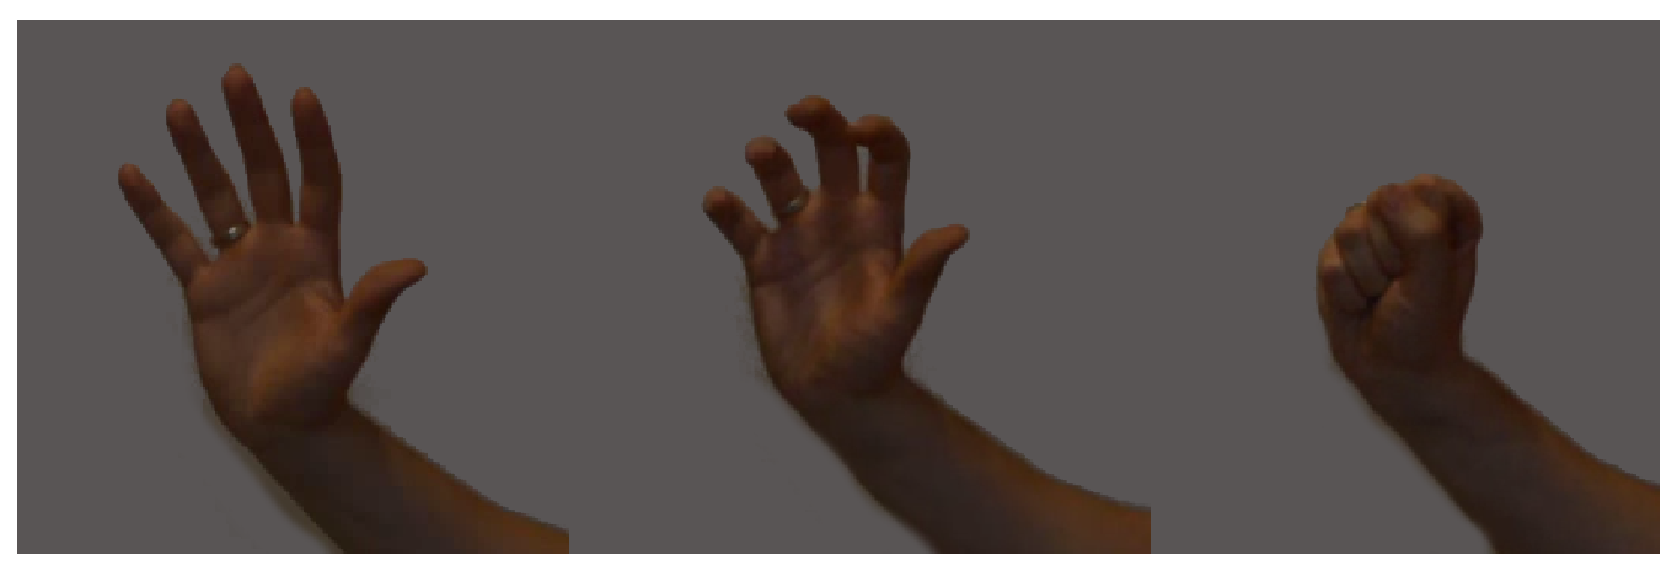
\includegraphics[height=1.5cm]{gestures/CrushGesture}
          \caption[Prezentacja gestu Zgniatanie]
                  {Prezentacja gestu \textit{Zgniatanie}}
          \label{fig:CrushGesture}
        \end{figure}

      \newpage
        \gest{Okrąg}
             {Gest wykonywany na jednolitej i~gładkiej powierzchni.}
             {Okrąg o~promieniu 20 cm.}
             {Prawa dłoń.}
             {Okrąg wykonywany do kamery otwartą dłonią.}
             {Kierunek ruchu jest zgodny z~ruchem wskazówek zegara.}
             {Dłoń znajduje się na godzinie dwunastej.}
             {Punkty charakterystyczne rozmieszczone równomiernie na krawędziach dłoni.}
             {Punkty wzorcowe połączone linią ciągłą rozmieszczone na okręgu co 30\degree.}

        \begin{figure}[!ht]
          \centering
          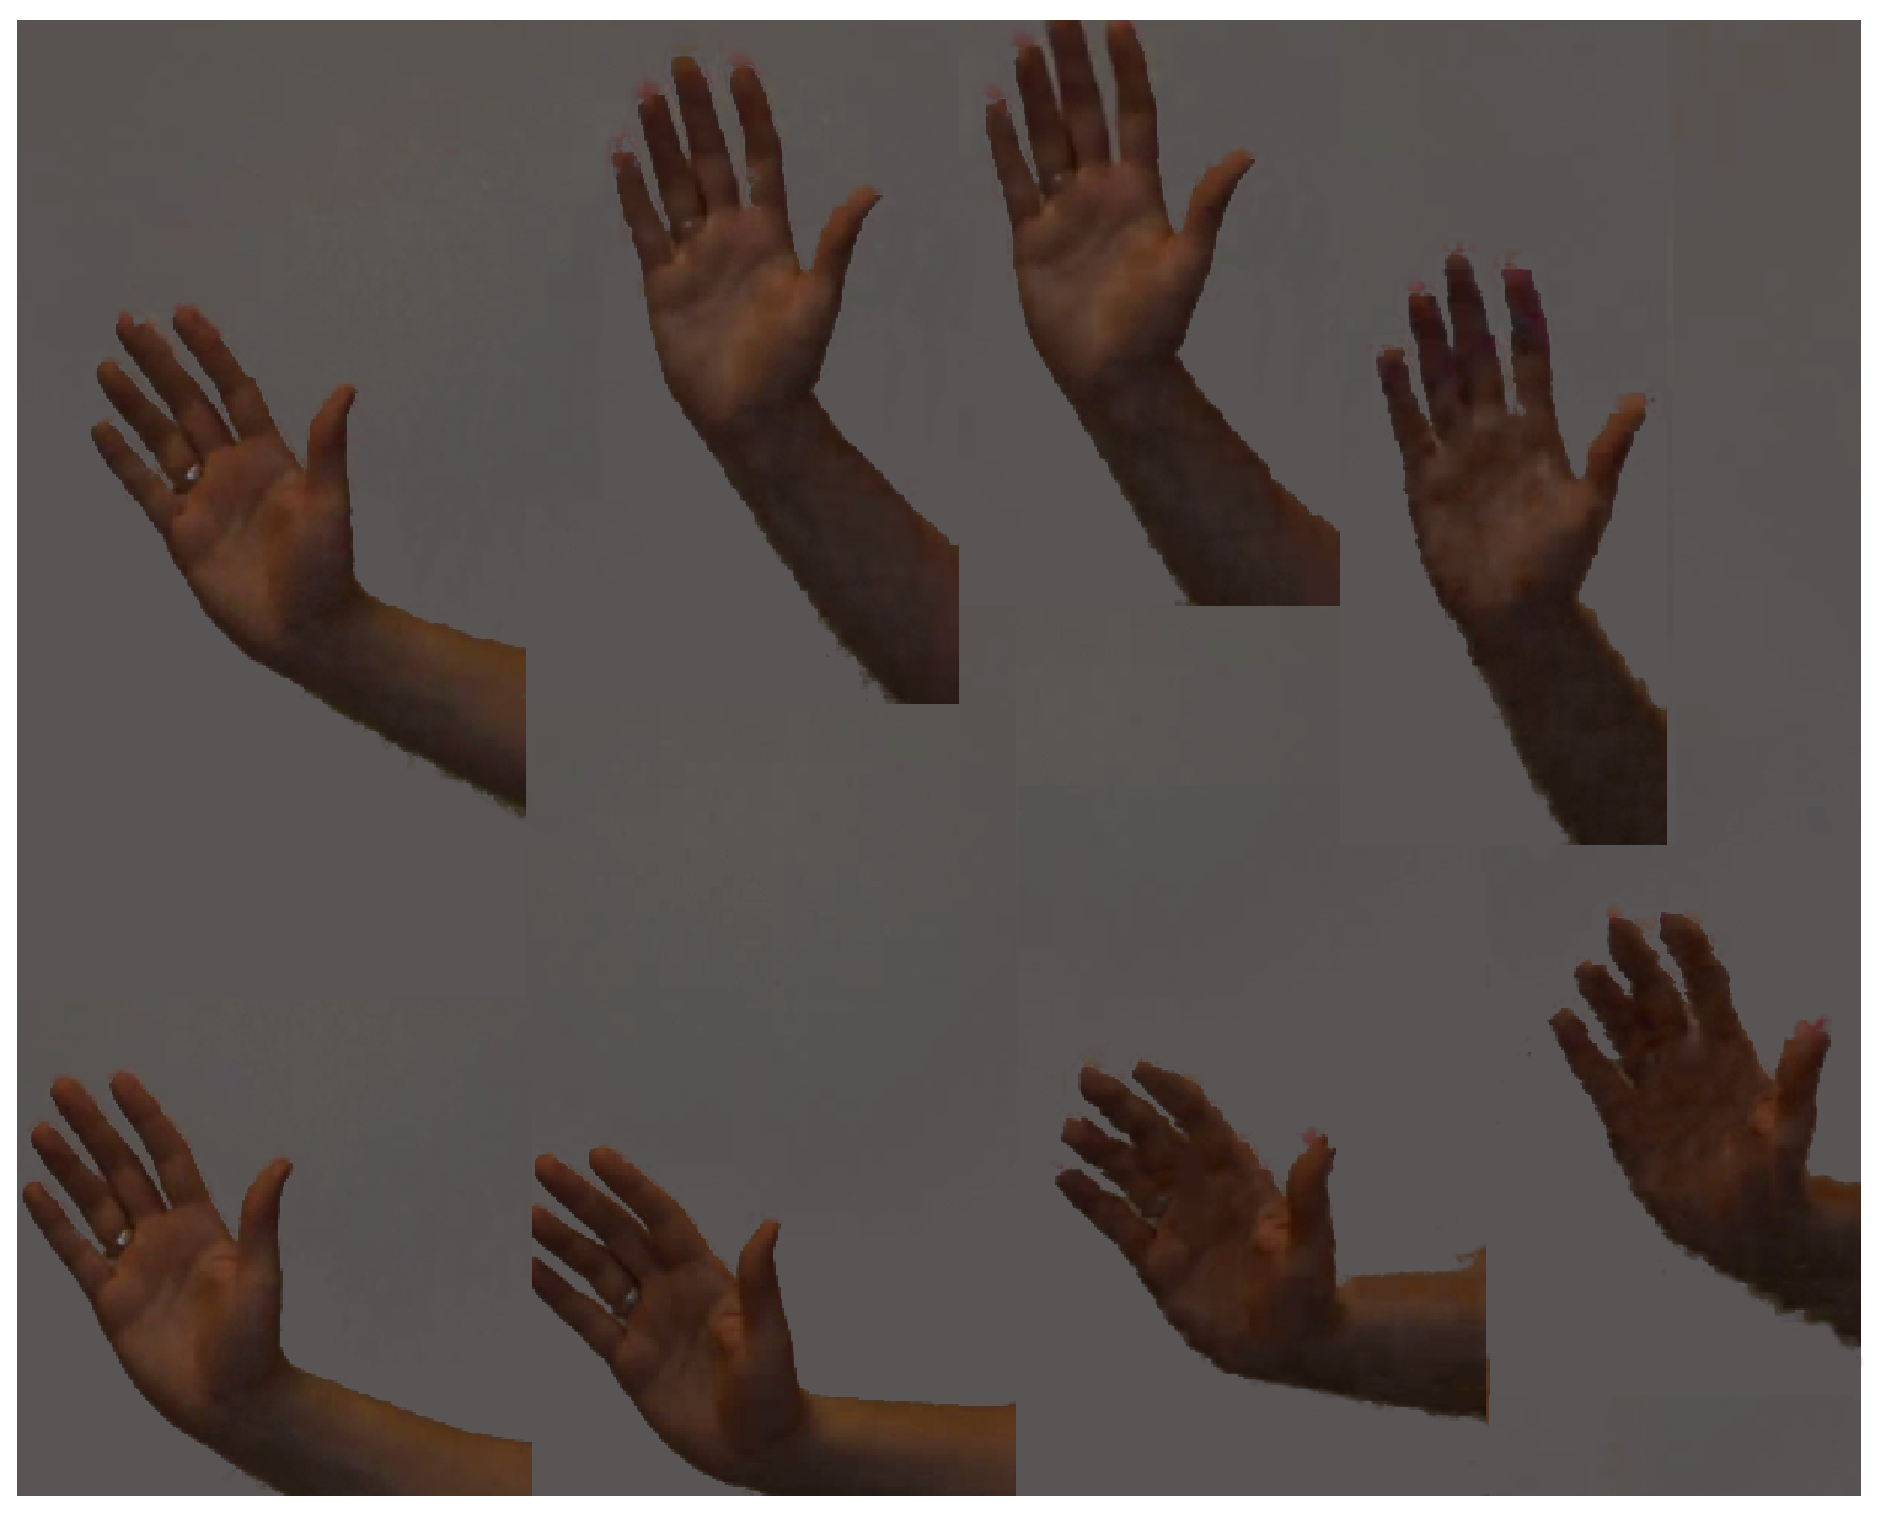
\includegraphics[height=7cm]{gestures/OGesture}
          \caption[Prezentacja gestu Okrąg]
                  {Prezentacja gestu \textit{Okrąg}}
          \label{fig:OGesture}
        \end{figure}

      \newpage
        \gest{Krzyż}
             {Gest wykonywany na jednolitej i~gładkiej powierzchni.}
             {Krzyż równoramienny o~promieniu 7 cm.}
             {Dwa, wyciągnięte palce (wskazujący oraz środkowy) prawej dłoni}
             {Kształt zarysowywany wewnętrzną stroną dłoni.}
             {W~pierwszej kolejności wykonywane jest ramię pionowe, następnie palce powracają do środka i~gest wykonywany jest w~lewą stronę a~następnie w~prawo.}
             {Ustawiona dłoń znajduje się na godzinie dwunastej.}
             {Punkty charakterystyczne rozmieszczone na czubkach wyciągniętych palców.}
             {5 punktów wzorcowych - cztery na krawędziach i~jeden w~środku figury.}

        \begin{figure}[!ht]
          \centering
          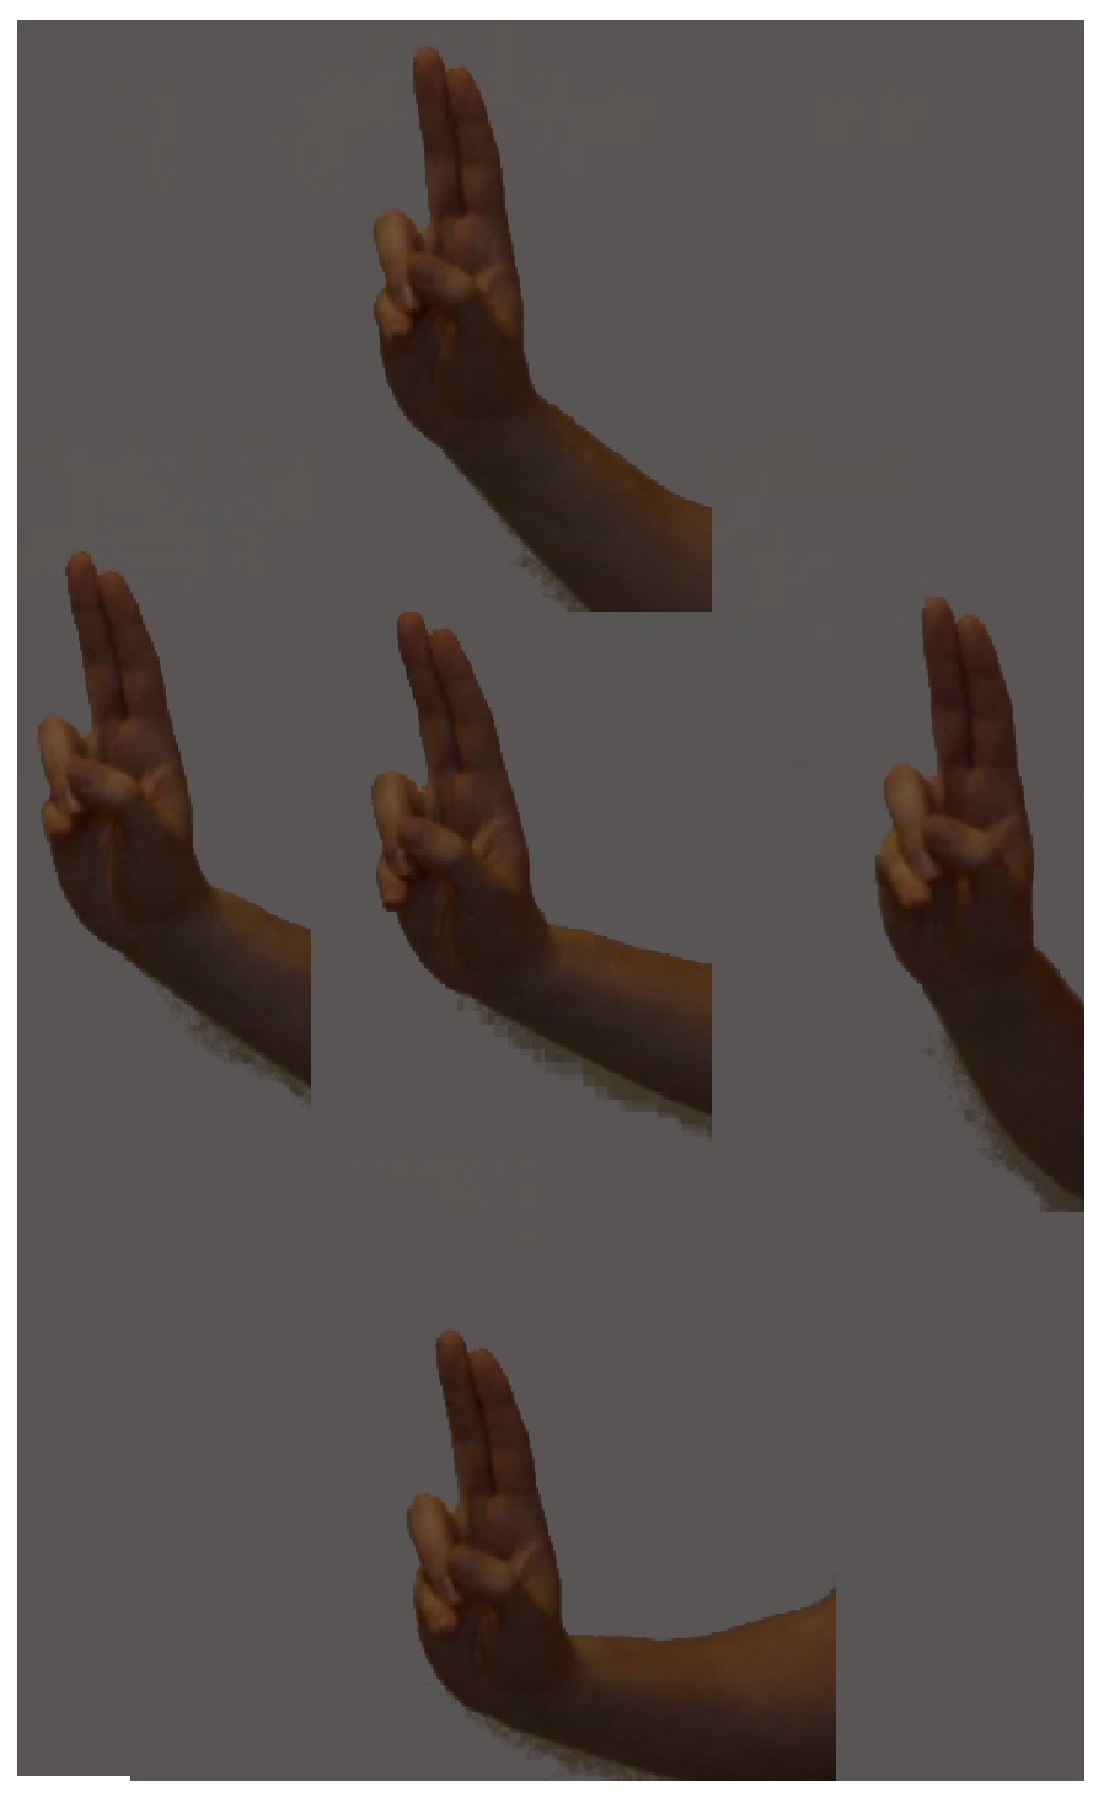
\includegraphics[height=7cm]{gestures/XGesture}
          \caption[Prezentacja gestu Krzyż]
                  {Prezentacja gestu \textit{Krzyż}}
          \label{fig:XGesture}
        \end{figure}

      \newpage
        \gest{Wielka litera C}
             {Gest wykonywany na jednolitej i~gładkiej powierzchni.}
             {Półokrąg o~promieniu 10 cm.}
             {Palec wskazujący lewej dłoni.}
             {Zarysowanie kształtu w~kierunku przeciwnym do ruchu wskazówek zegara.}
             {Gest powinien być wykonywany przez poruszenie całej dłoni, nie tylko samego palca.}
             {Palec wskazujący na godzinie dwunastej.}
             {Punkty charakterystyczne zaznaczone na krawędziach analizowanego palca.}
             {Punkty połączone linią ciągłą rozmieszczone równomiernie na półokręgu co 30\degree.}

        \begin{figure}[!ht]
          \centering
          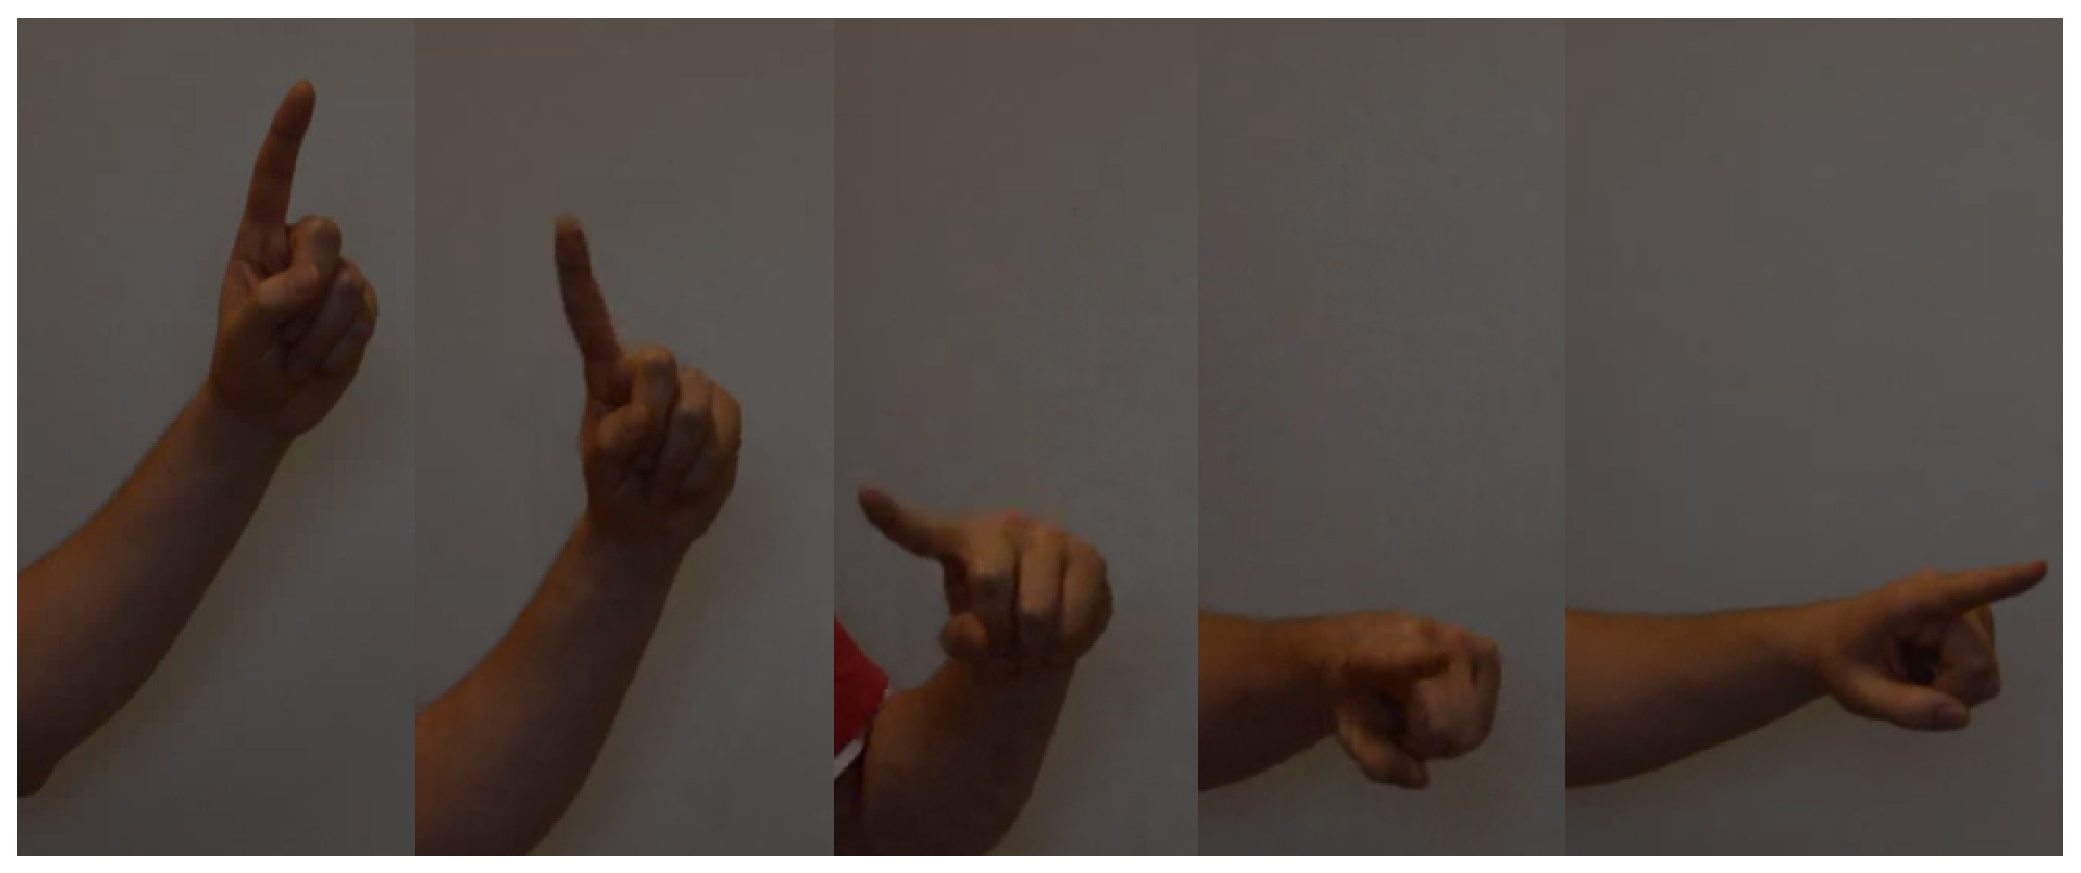
\includegraphics[height=6cm]{gestures/CGesture}
          \caption[Prezentacja gestu Wielka litera C]
                  {Prezentacja gestu \textit{Wielka litera C}}
          \label{fig:CGesture}
        \end{figure}

      \newpage
        \gest{Wielka litera L}
             {Gest wykonywany na jednolitej i~gładkiej powierzchni.}
             {Litera L o~wysokości 7 cm.}
             {Złączone palce prawej dłoni.}
             {Kształt litery zarysowują czubki palców.}
             {Gest powinien być wykonywany przez poruszanie tylko złączonymi palcami, nie samą dłonią.}
             {Palce na godzinie dwunastej.}
             {Punkty charakterystyczne rozmieszczone równomiernie na górnej części dłoni.}
             {4 punkty wzorcowe - na początku, na końcu, na zgięciu litery oraz dodatkowy punkt na dłuższej części litery, dokładnie w~jej połowie.}

        \begin{figure}[!ht]
          \centering
          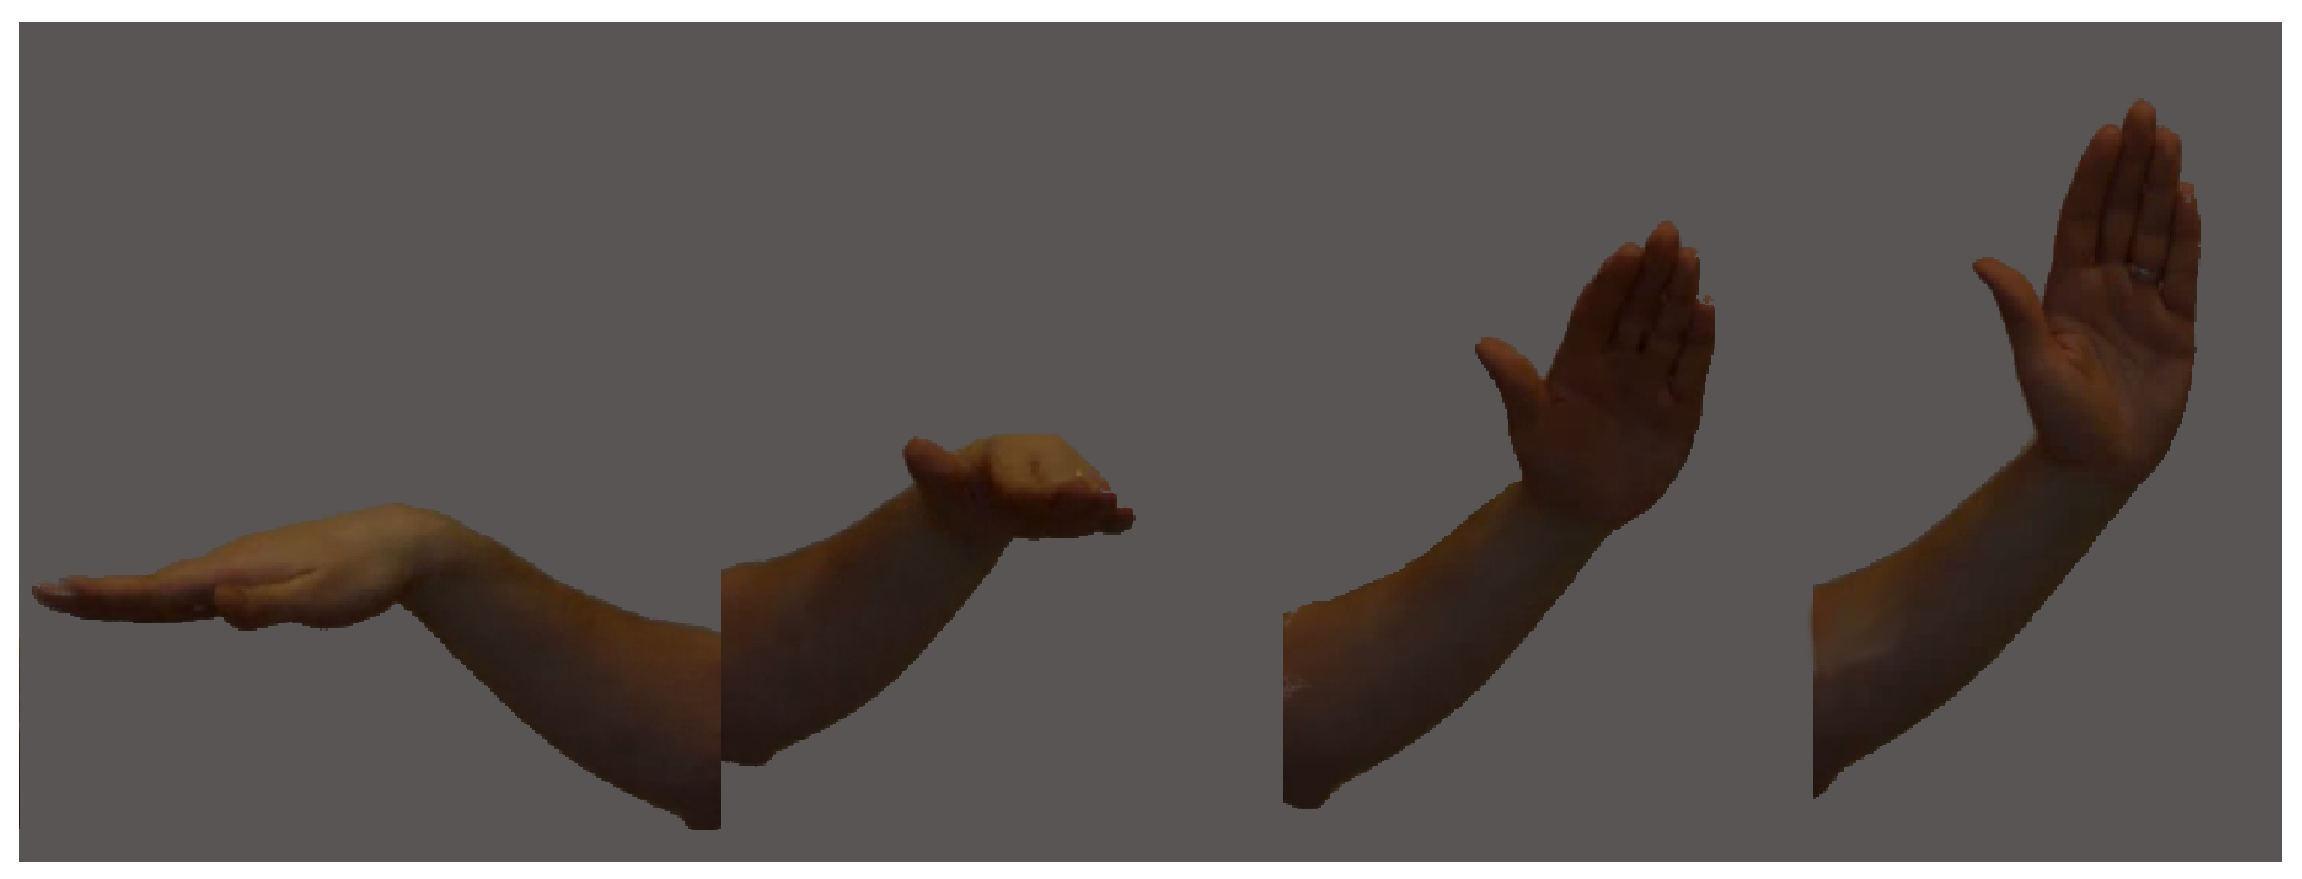
\includegraphics[height=4cm]{gestures/LGesture}
          \caption[Prezentacja gestu Wielka litera L]
                  {Prezentacja gestu \textit{Wielka litera L}}
          \label{fig:LGesture}
        \end{figure}

      \newpage
        \gest{Rozszerzanie}
             {Gest wykonywany na tle twarzy lub ciała.}
             {W~pozycji wyjściowej, jest to kwadrat o~długości boku około 20 cm.}
             {Obie dłonie złączone czubkami palców uformowane w~gest \textit{szczypty}.}
             {Oburęczny gest rozciągania dłoni od środka.}
             {Gest powinien symulować rozciąganie niewidzialnego materiału. Kształt dłoni nie powinien ulegać zmianie w~trakcie wykonywania gestu.}
             {Obie złączone dłonie znajdują się w~środku figury na wysokości klatki piersiowej.}
             {Punkty charakterystyczne rozmieszczone równomiernie na powierzchni obu dłoni.}
             {Punkty wzorcowe równomiernie rozmieszczone na przekątnej kwadratu.}

        \begin{figure}[!ht]
          \centering
          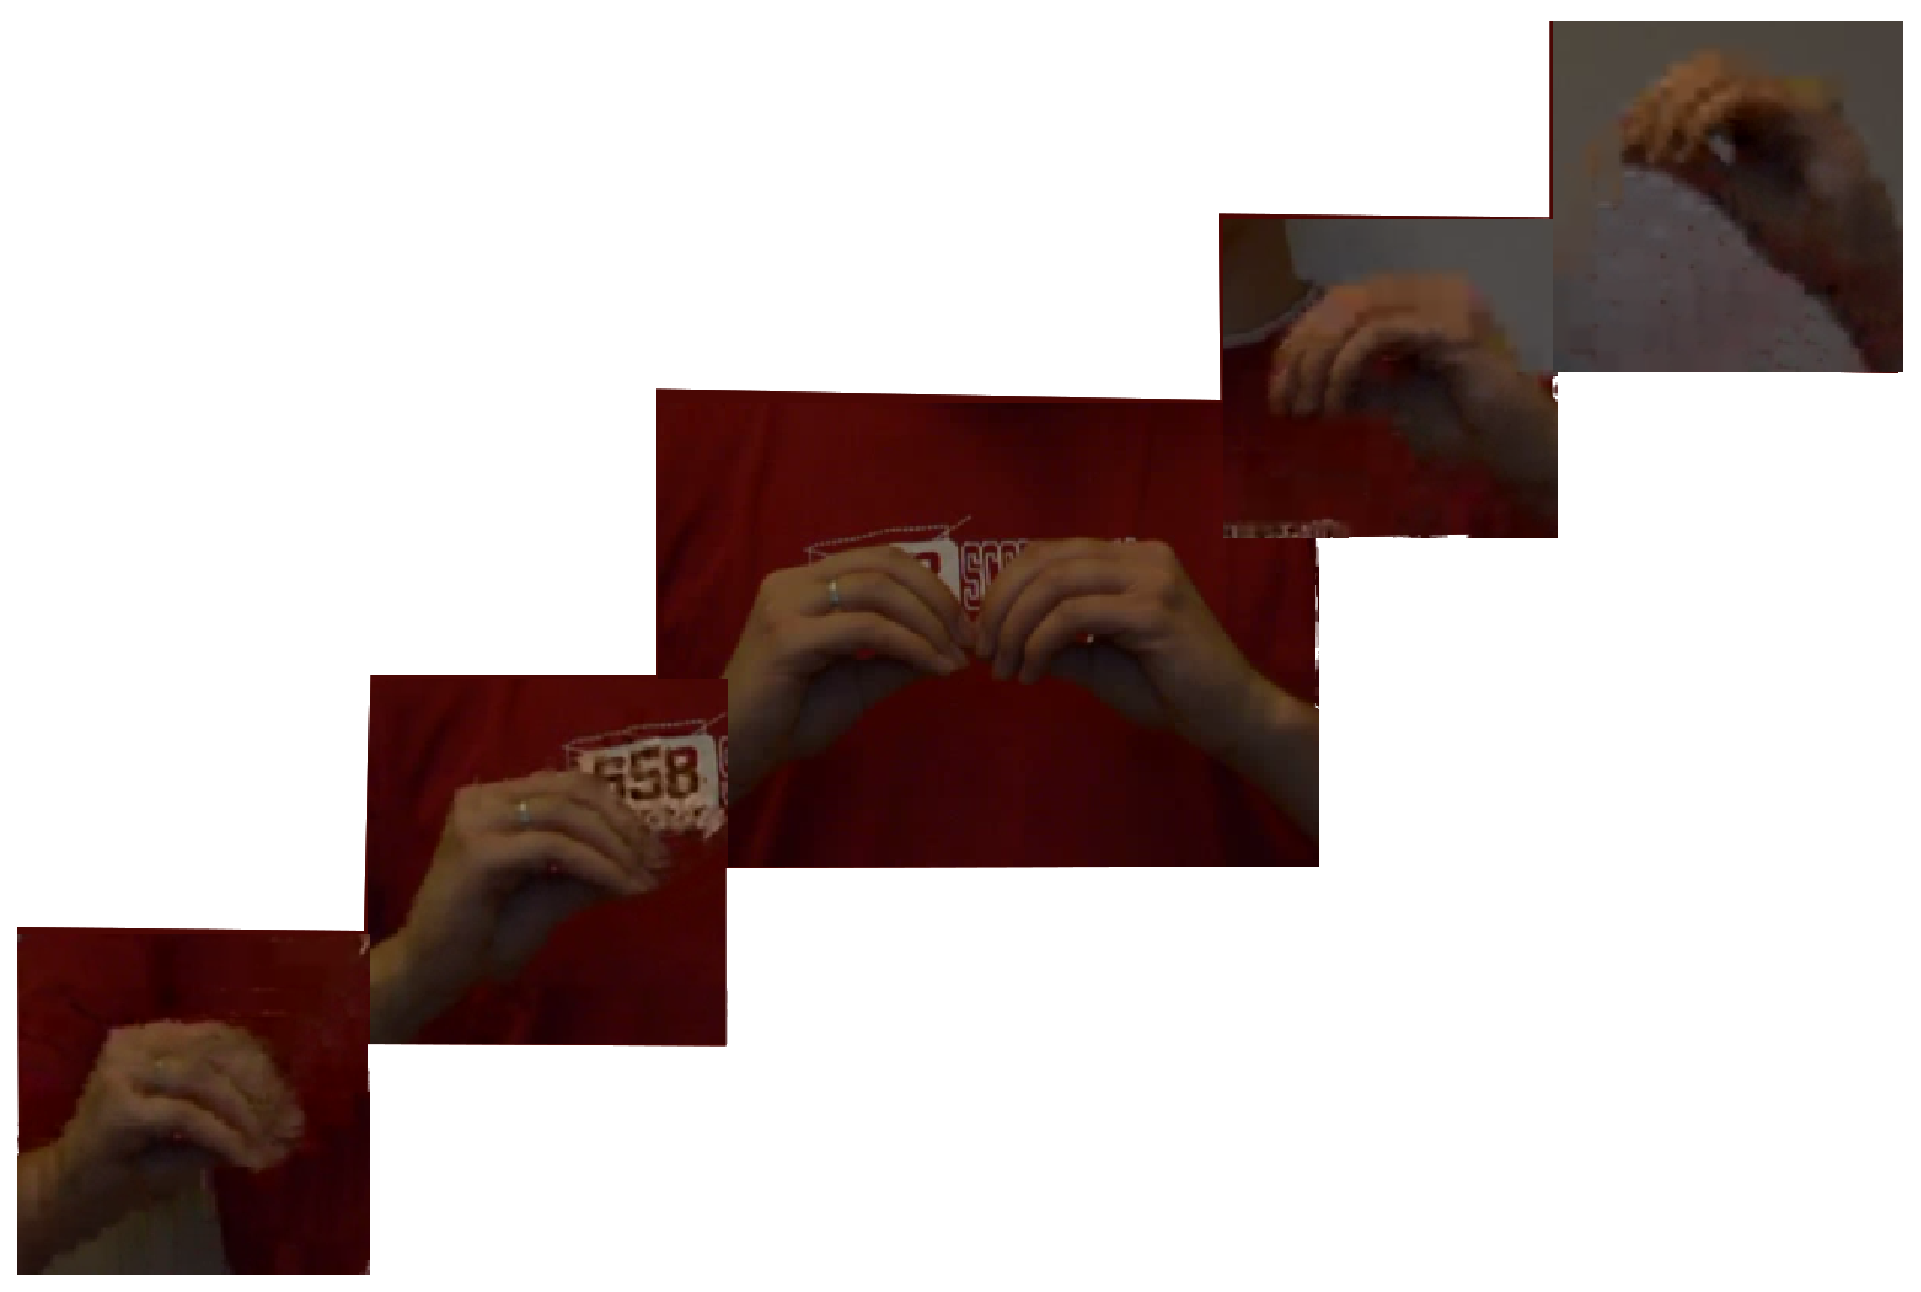
\includegraphics[width=10cm]{gestures/StretchGesture}
          \caption[Prezentacja gestu Rozszerzanie]
                  {Prezentacja gestu \textit{Rozszerzanie}}
          \label{fig:StretchGesture}
        \end{figure}

    \subsection{Akwizycja i~obróbka danych wejściowych}\label{Subsection_Akwizycja}

      Przed przeprowadzeniem badań zostały zebrane dane wejściowe w~postaci sekwencji wideo, dokumentujące gesty wykonywane według powyższego protokołu. Proces akwizycji został przeprowadzony na grupie 10 osób, każda z~nich wykonała 6~gestów. Cała procedura wykonywana była w~warunkach normalnego oświetlenia dziennego z~dodatkowym sztucznym oświetleniem umiejscowionym ponad stanowiskiem.

      Stanowisko akwizycji złożone było z~aparatu fotograficznego \textit{Nikon D7000}, popularnie zwanego \textit{lustrzanką}, wraz z~obiektywem \textit{Nikkor} o~ogniskowej 50~mm oraz wartość przysłony obiektywu $1:1.4$. Sam aparat cyfrowy posiada matrycę \textit{CMOS} o~rozdzielczości $16.2$~MP oraz był wyposażony w~kartę pamięci typu \textit{SD} o~dużej prędkości zapisu oraz odczytu wynoszącej 95~MB/s. Lustrzanka umieszczona była na statywie na wysokości klatki piersiowej filmowanej osoby w~pozycji pionowej.

      Sekwencja wideo była nagrywana w~rozdzielczości 1280 na 720 pikseli (720 linii poziomych obrazu), bez przeplotu z~częstotliwością 25 klatek na sekundę. Podczas nagrywania wszystkich sekwencji parametr przysłony wynosił 3.5, czas naświetlania był równy $1/320$ s oraz parametr \textit{ISO} posiadał wartość 320.

      Po przeprowadzeniu akwizycji, wyselekcjonowaniu odpowiednich próbek i~nazwaniu ich wszystkie sekwencje wideo zostały przekształcone z~oryginalnego formatu \textit{MOV} (kodek \textit{h264}) na format \textit{AVI} (kodek \textit{MPEG 4.2}) za pomocą skryptu \ref{MOVtoAVIConversion} zamieszczonego również na płycie dołączonej do pracy. Warto zauważyć, że podczas konwersji obraz został również obrócony o~90\degree~przeciwnie do ruchu wskazówek zegara, aby uzyskać naturalne (pionowe) ułożenie zapisanej sekwencji wideo.

        \begin{sample}[ht]
          \begin{verbatim}
  #!/bin/sh

  # ...

  pushd "PersonA"

  for file in *.MOV; do
    ffmpeg -i "$file" -q:v 0 -vf "transpose=2"
           -vcodec msmpeg4v2 ../../Person_A_${file%%.*}.avi
  done

  popd
          \end{verbatim}
          \caption{Fragment skryptu konwertującego pliki MOV do formatu AVI}
          \label{MOVtoAVIConversion}
        \end{sample}

    \subsection{Ocena jakości algorytmu śledzenia}\label{Subsection_Jakosc}

      W~celu analizy i~porównania jakości poszczególnych algorytmów przygotowano zestaw parametrów, które będą badane podczas wykonania każdego z~nich. Główną rolę odgrywają tutaj \textit{punkty wzorcowe} oraz \textit{połączenia} między nimi.

      Jakość algorytmu wyznaczana będzie na podstawie odchyleń tras oraz pozycji punktów charakterystycznych w~stosunku do pozycji punktów wzorcowych oraz tras pomiędzy nimi.

      Każdy z~gestów posiada serię punktów wzorcowych połączonych ze sobą liniami prostymi (w~celu symulacji gładszych połączeń np. okręgu stosuje się odpowiednią liczbę punktów pośrednich). Każdy z~punktów wzorcowych oprócz swojej pozycji posiada również \textit{okrąg otaczający} o~określonym promieniu.

      W~określonych przez punkty wzorcowe klatkach animacji następuje przeszukanie wszystkich dostępnych w~danej chwili czasu \textit{t} punktów charakterystycznych i~obliczana jest ich odległość od punktu wzorcowego. Do porównania wybierany jest najbliższy punkt zgodnie z~metryką euklidesową, co formalnie zostało zdefiniowane jako \textbf{odchylenie minimalne od punktu wzorcowego} w~następujący sposób:

        \begin{equation}
          \forall_{k\in K} \; \forall_{s \in S_{t}} \; min\{ d(k, s) \},
        \end{equation}
      gdzie $K$ to zbiór punktów wzorcowych, $S_{t}$ to zbiór punktów charakterystycznych w~chwili $t$ oraz~$d$ to metryka euklidesowa.

      W~klatkach pośrednich analizowana jest odległość wszystkich punktów charakterystycznych od aktualnej \textit{trasy}. Dzięki temu wiadomo jak wygląda dystrybucja punktów charakterystycznych wokół śledzonej trasy. Zapis formalny jest analogiczny do powyższego i~został zdefiniowany jako \textbf{odchylenie minimalne od trasy wzorcowej} w~następujący sposób:

        \begin{equation}
          \forall_{p\in P} \; \forall_{s \in S_{t}} \; min\{ d(p, s) \},
        \end{equation}
      gdzie $P$ to zbiór tras wzorcowych, $S_{t}$ to zbiór punktów charakterystycznych w~chwili $t$ oraz~$d$ to metryka euklidesowa.

      Warto zauważyć, że taki sposób weryfikacji odporny jest na zmiany (poprzez dokładanie lub usuwanie) punktów charakterystycznych.

      Biorąc pod uwagę dwa wspomniane parametry tj. \textbf{odchylenie minimalne od punktu wzorcowego w~danej klatce sekwencji wideo} oraz \textbf{wektor odchyleń punktów charakterystycznych od trasy} można skutecznie porównać jakość badanych algorytmów między sobą.

    \subsection{Ocena wydajności algorytmu śledzenia}\label{Subsection_Wydajnosc}

      W~celu analizy i~porównania wydajności poszczególnych algorytmów przygotowano zestaw wyznaczników, które obliczane będą podczas wykonania każdego algorytmu. Ujednolicenie to ma celu wypracowanie wspólnego wzorca porównawczego różnych algorytmów o~zupełnie innej zasadzie działania oraz implementacji.

      Główne parametry porównawcze opierają się na pomiarach czasu wykonania oraz własnościami statystycznymi wyciągniętymi z~pomiarów.

      Pierwszy pomiar to \textbf{czas przetwarzania pojedynczej klatki}. Z~wartości pomiarów dla wszystkich klatek sekwencji wideo wyciągnięte zostaną własności statystyczne tj. \textit{średnia arytmetyczna}, \textit{mediana}, \textit{odchylenie standardowe}.

      Kolejnym pomiarem jest \textbf{sumaryczny czas przetwarzania algorytmu}. Warto zauważyć, że nie będzie on nigdy mniejszy od nominalnego czasu trwania sekwencji wideo. Sumaryczny czas może być jedynie równy wartości nominalnej w~przypadku, gdy przetwarzanie pojedynczej klatki wideo odbędzie się w~czasie mniejszym bądź równym wartości niezbędnej do odczekania przed wyświetleniem następnej klatki. Czasu oczekiwania jest ściśle związany z~wartością \textit{częstotliwości klatek na sekundę} analizowanej sekwencji wideo.

      Następna wartość to \textbf{odchylenie sumarycznego czasu wykonania od czasu nominalnego} wyrażona w~procentach.

      Ostatni wyznacznik to klasyfikacja algorytmów według stopnia ich złożoności. Każdy algorytm będzie poddany analizie pod kątem wyselekcjonowanego zbioru operacji dominujących, w~celu wyznaczenia \textbf{złożoności obliczeniowej oraz pamięciowej}.

  \section{Opis wygenerowanych zbiorów i~rezultatów}\label{Section_Results}
    Zanim zostaną dokładnie omówione i~przeanalizowane wyniki przeprowadzonych badań, warto przybliżyć kilka szczegółów dotyczących zebranych rezultatów.

    Wszystkie wyniki zostały zebrane z~plikach z~rozszerzeniem JSON (są to samoopisujace się pliki tekstowe ogólnego przeznaczenia, oparte na strukturze słownika typu \textit{klucz} - \textit{wartość}). Rozmiar wygenerowanych danych wynosi $4,1$ MB, co jak na dane czysto tekstowe jest dość dużą liczbą (ponad 4 miliony znaków).

    Czas trwania podstawowych testów (analiza wszystkich zebranych próbek - 3 różne algorytmy o~domyślnych parametrach, 10 osób po 6 gestów) to ponad dwie i~pół godziny. Dla wyspecjalizowanych przypadków czas przetwarzania wyniósł trzy i~pół godziny (wybrane parametry dla 3 algorytmów na 2 najlepszych jakościowo próbkach 2 gestów). Przypadki dodatkowe zostały zebrane w~pliku \textit{parametrized.json} umieszczonym w~katalogu głównym kodu źródłowego.

    W~przypadku algorytmu opartego na uczeniu maszynowym, rozmiar wygenerowanych zbiorów treningowych dla domyślnych parametrów (las złożony z~5~drzew losowych, 200 punktów charakterystycznych, wymiar boku kwadratowej łaty - 20 pikseli) wyniósł dokładnie $43$ GB. Czas generacji został uwzględniony w~powyższym akapicie.

    Rezultaty zostały zebrane za pomocą 64 wykresów, analizujących cztery różne obszary porównawcze, tj.:
      \begin{itemize}
        \item Zużycie pamięci wirtualnej i~fizycznej.
        \item Wydajność (czas przetwarzania klatki animacji oraz czas dodatkowych operacji niezbędnych do obliczeń).
        \item Narzut czasowy obliczeń, wprowadzony do nominalnego czasu trwania sekwencji wideo.
        \item Jakość wygenerowanej ścieżki w~stosunku do wyznaczonych manualnie punktów i~ścieżek wzorcowych.
      \end{itemize}

    W~kolejnych sekcjach zostały szczegółowo omówione wyniki oraz przedstawione wnioski dla każdego z~analizowanych obszarów.

  \section{Zużycie pamięci badanych algorytmów}\label{Section_Memory}

    Zaimplementowane algorytmy posiadają zupełnie trzy odrębne profile pamięciowe co zamieszczone zostało na wykresach \ref{fig:MemoryUsagePersonAC} oraz \ref{fig:MemoryUsagePersonGC}, reprezentujących dwie odrębne próbki. W~przypadku metod opartych o~rodzinę algorytmów przepływu optycznego wartość zużywanej pamięci nie różni się pomiędzy poszczególnymi próbkami. Dla trzeciego algorytmu zużycie waha się w~przedziale od $350$ do $800$ MB dla pamięci wirtualnej i~dla pamięci fizycznej w~przedziale od $150$ do $600$ MB. Widać wyraźnie, że najwięcej pamięci pochłania implementacja opierająca się algorytmie wykorzystującym las drzew losowych i~ilość zaalokowanej pamięci zależy ściśle od przygotowanej bazy treningowej oraz parametrów próbki wideo.

      \begin{figure}[!ht]
        \centering
        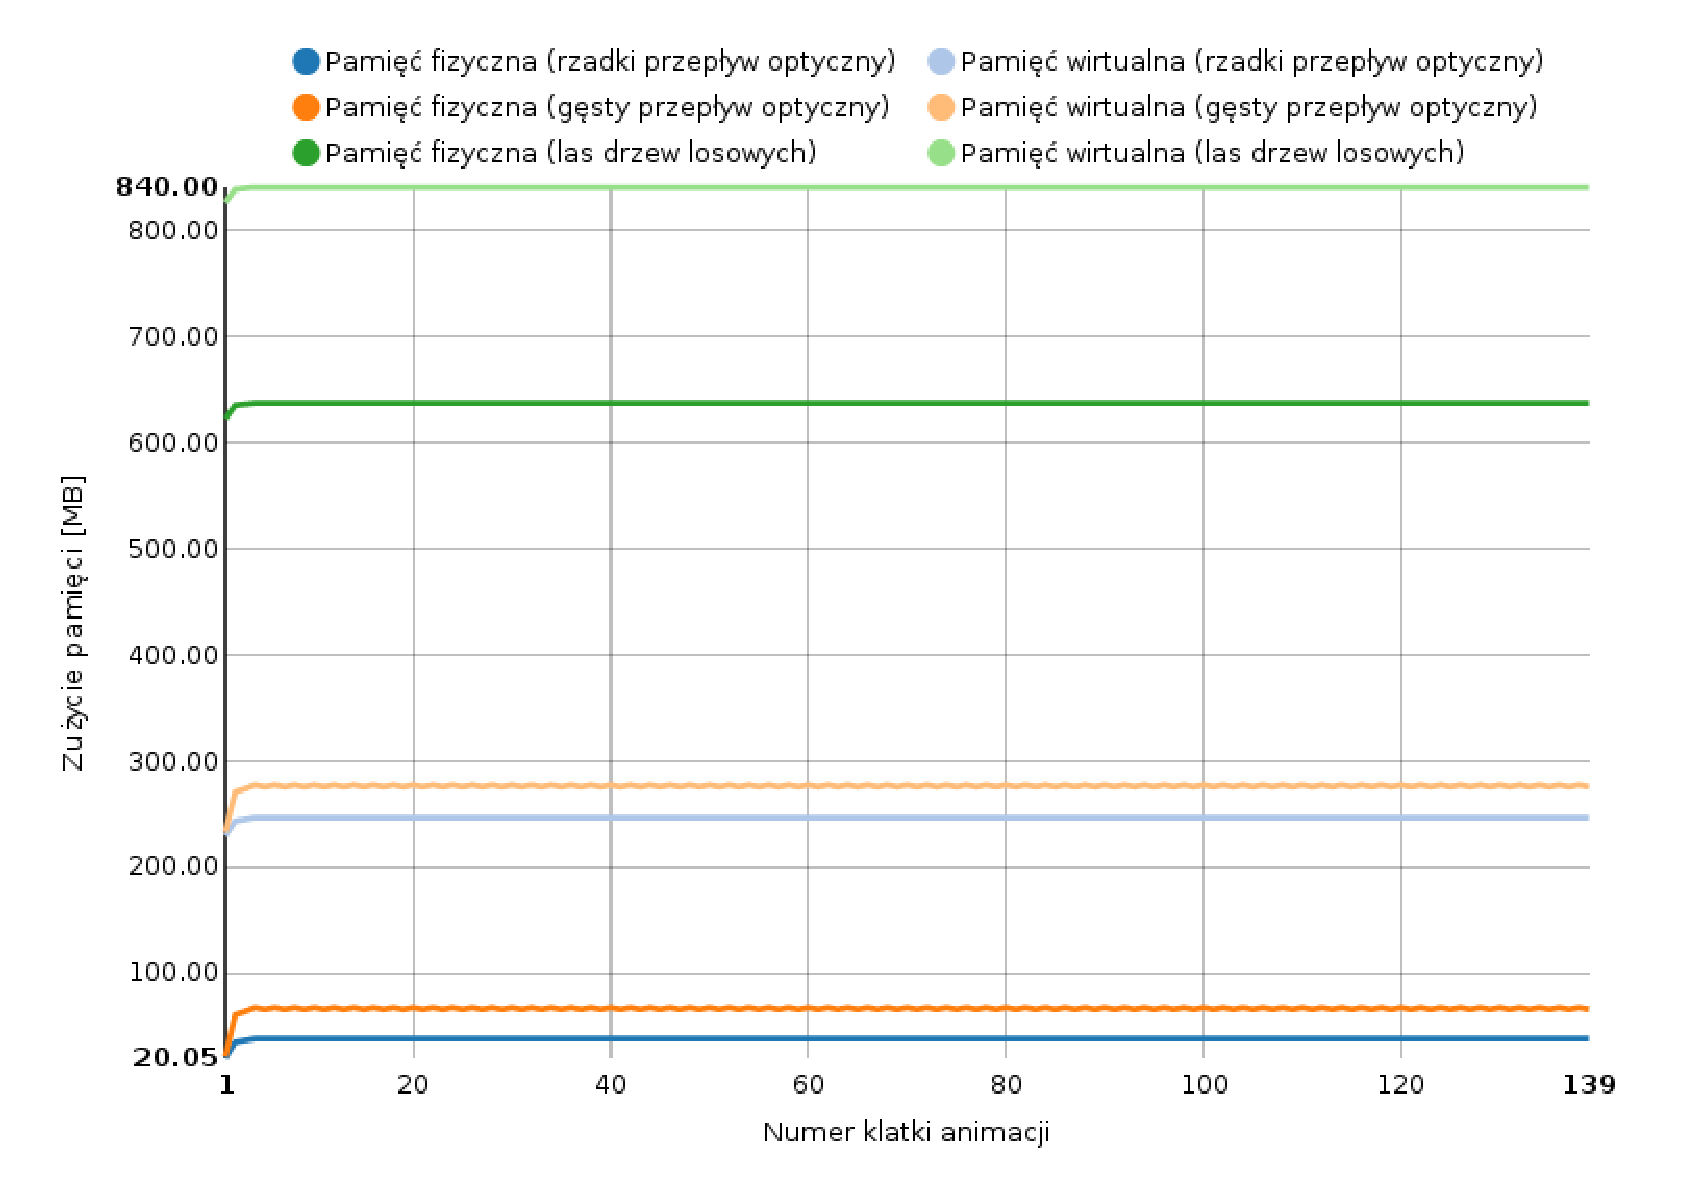
\includegraphics[width=14cm]{charts/memory/PersonAC}
        \caption[Wykres zużycia pamięci dla próbki o nazwie Person\_A\_C]
                {Wykres zużycia pamięci dla próbki o nazwie \textit{Person\_A\_C}}
        \label{fig:MemoryUsagePersonAC}
      \end{figure}

    W~przypadku gęstego przepływu optycznego zużycie pamięci fizycznej nie przekracza $80$ MB, dla implementacji algorytmu opartego o~metodę \textit{LK} osiąga wartość co najwyżej $50$ MB. Oba algorytmy są zdecydowanie oszczędniejsze od trzeciej zaproponowanej implementacji.

      \begin{figure}[!ht]
        \centering
        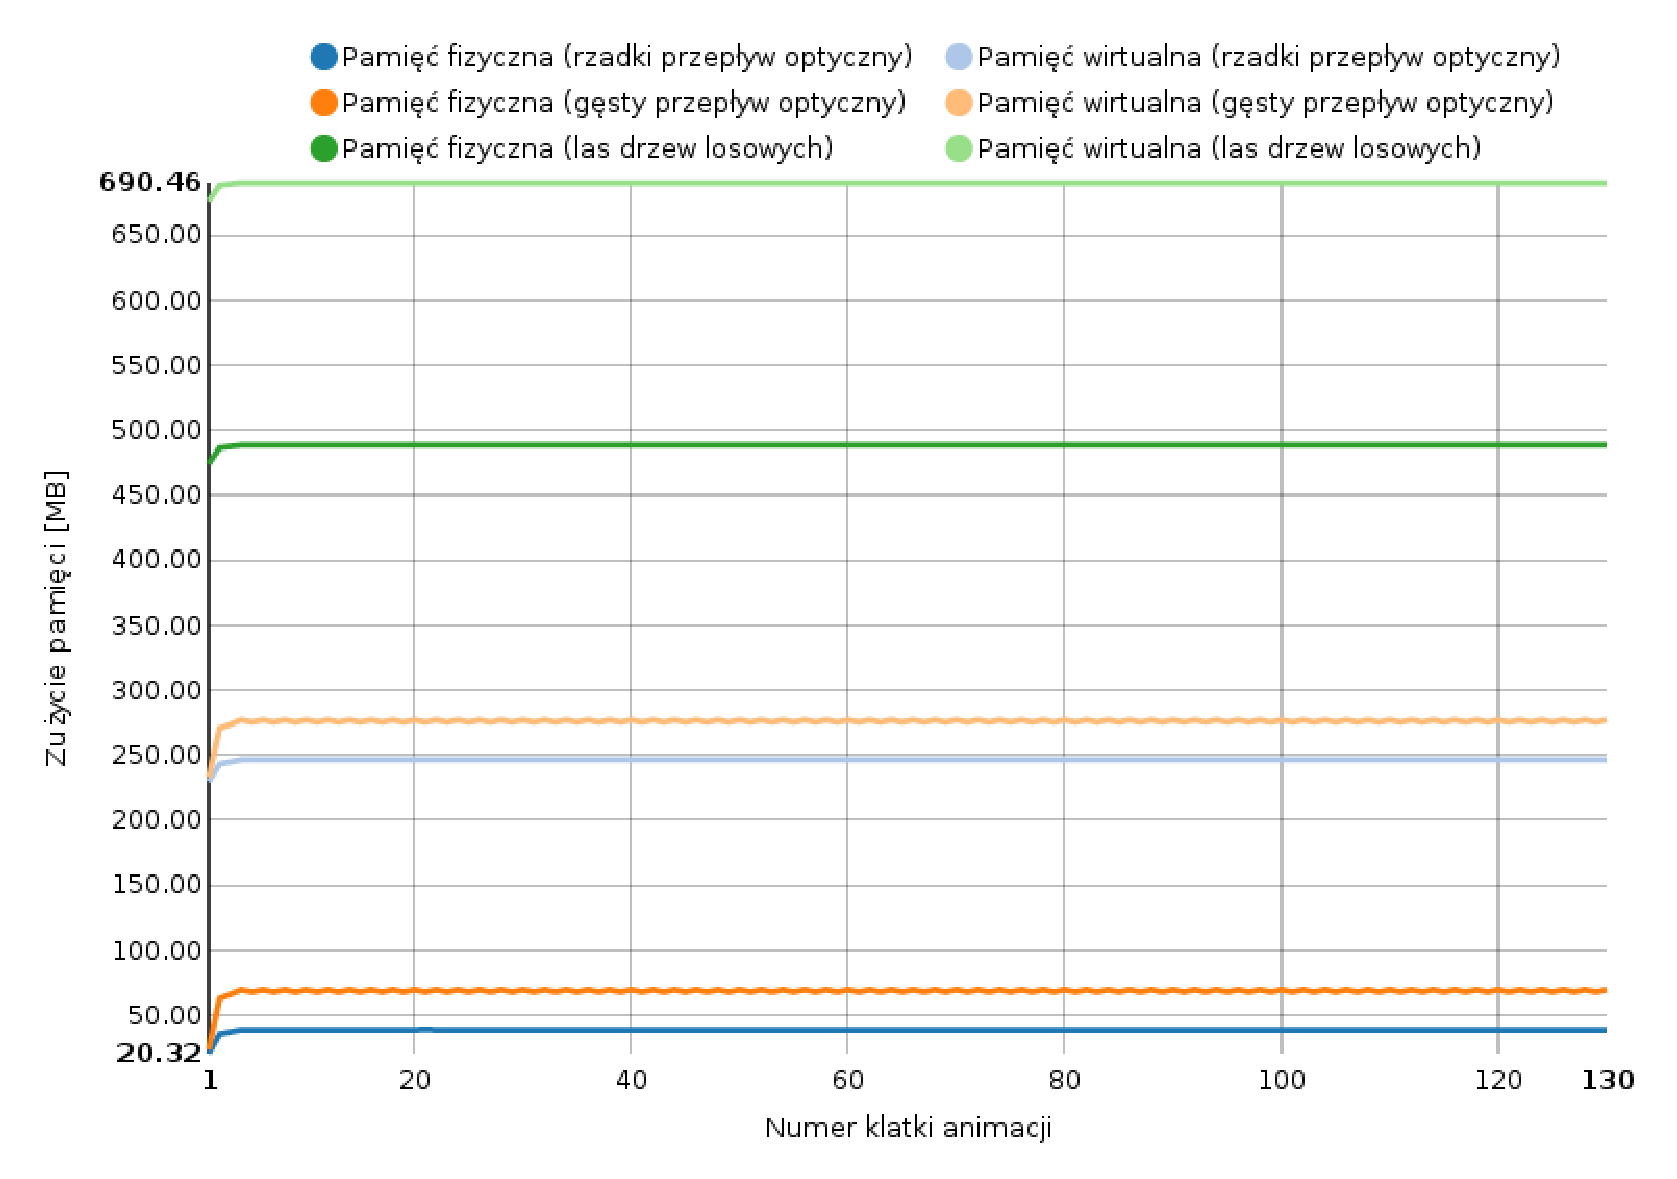
\includegraphics[width=14cm]{charts/memory/PersonGC}
        \caption[Wykres zużycia pamięci dla próbki o nazwie Person\_G\_C]
                {Wykres zużycia pamięci dla próbki o nazwie \textit{Person\_G\_C}}
        \label{fig:MemoryUsagePersonGC}
      \end{figure}

    Algorytm gęstego przepływu optycznego posiada jedną wadę - mimo stosunkowo niewielkiego zużycia pamięci, na wykresie \ref{fig:OpticalFlowsMemoryUsage} został zaprezentowany piłokształtny przebieg, ciągłej alokacji i~zwalniania od 2 do 4 MB bufora pamięci pomiędzy poszczególnymi klatkami sekwencji wideo. Nie jest to korzystne zjawisko i~jego eliminacja na pewno wpłynie pozytywnie na całkowitą wydajność.

      \begin{figure}[!ht]
        \centering
        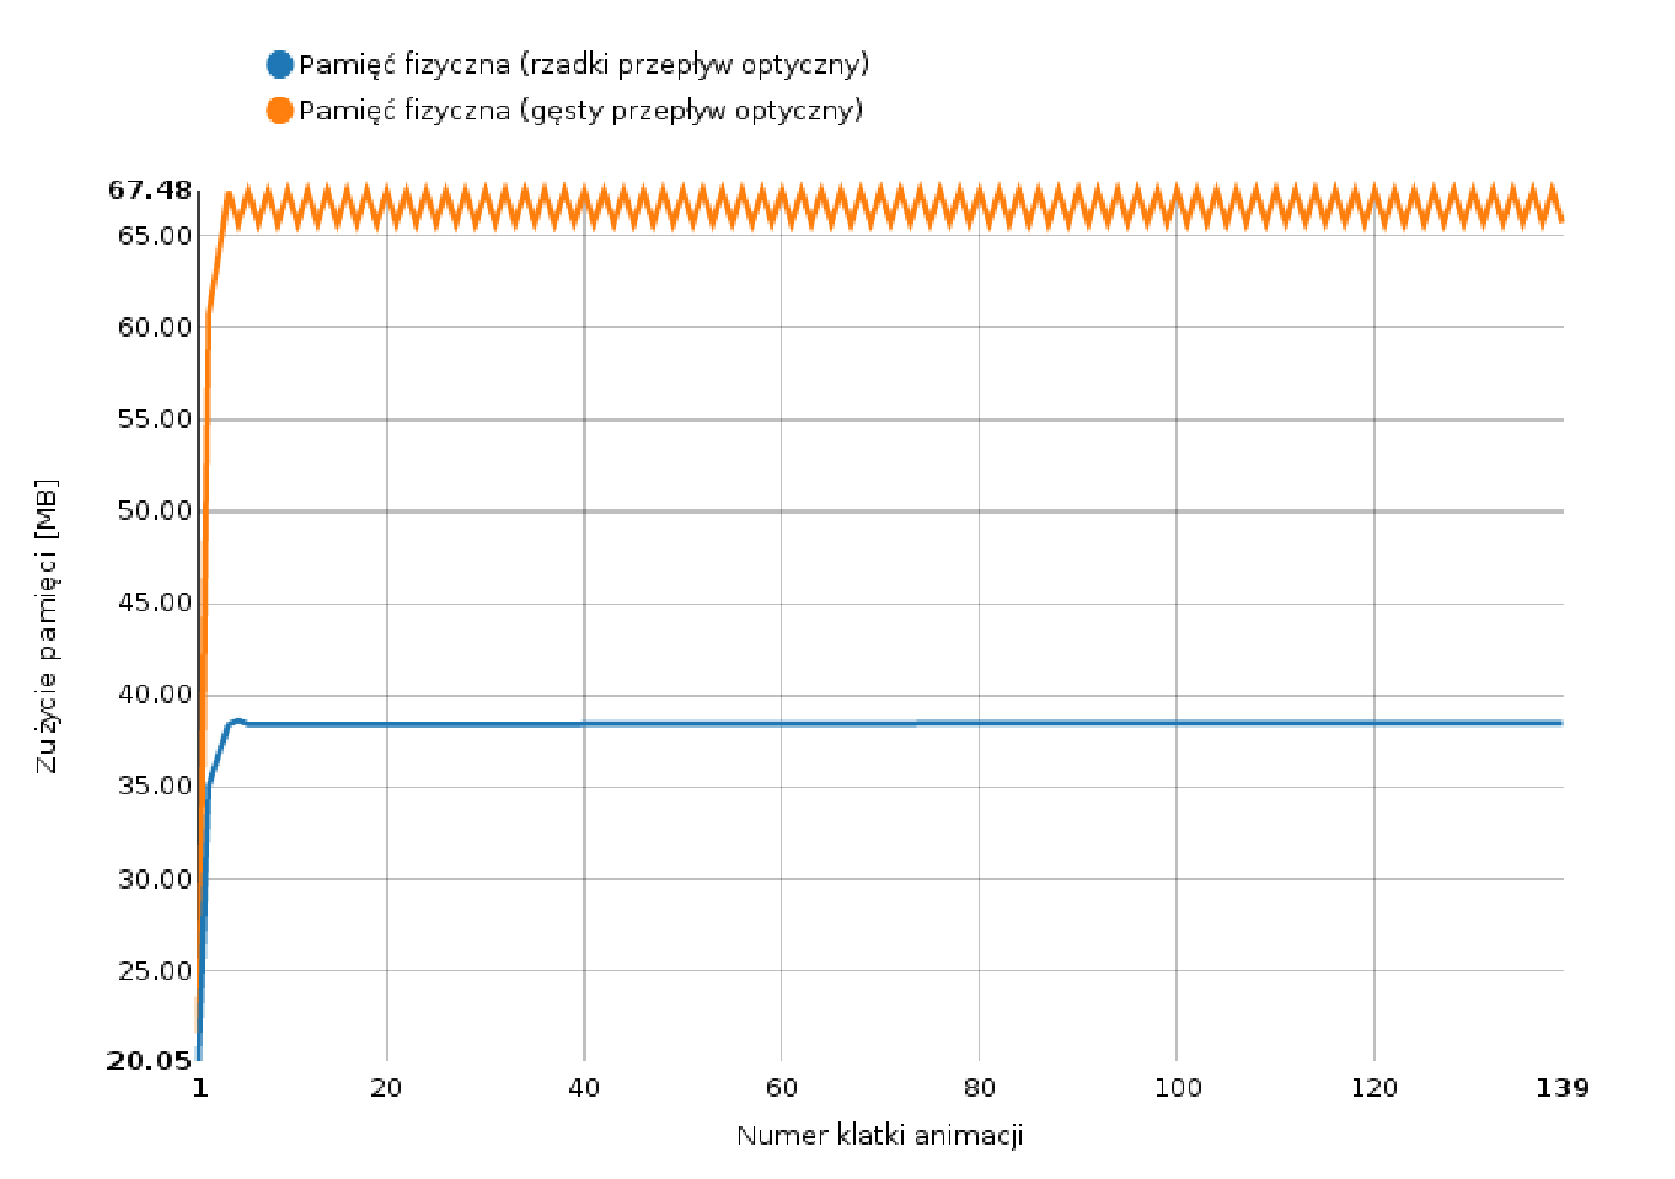
\includegraphics[width=14cm]{charts/memory/OpticalFlows}
        \caption[Wykres zużycia pamięci dla algorytmów przepływu optycznego]
                {Wykres zużycia pamięci dla algorytmów przepływu optycznego}
        \label{fig:OpticalFlowsMemoryUsage}
      \end{figure}

    W~przypadku algorytmu opartego o~las drzew losowych zużycie pamięci liniowo zależy od liczby wytrenowanych drzew wykorzystanych do budowy klasyfikatora. Zależność została zaprezentowana na rysunku \ref{fig:RandomForestTrackerPerTrainedTreesAmount}. Jednocześnie można zauważyć, że różnica pomiędzy minimalnym i~maksymalnym zużyciem pamięci jest niewielka co oznacza, że proces potrzebuje dużej ilości pamięci, ale nie jest algorytmem intensywnym w~operacje przydzielania i~zwalniania zasobów.

      \begin{figure}[!ht]
        \centering
        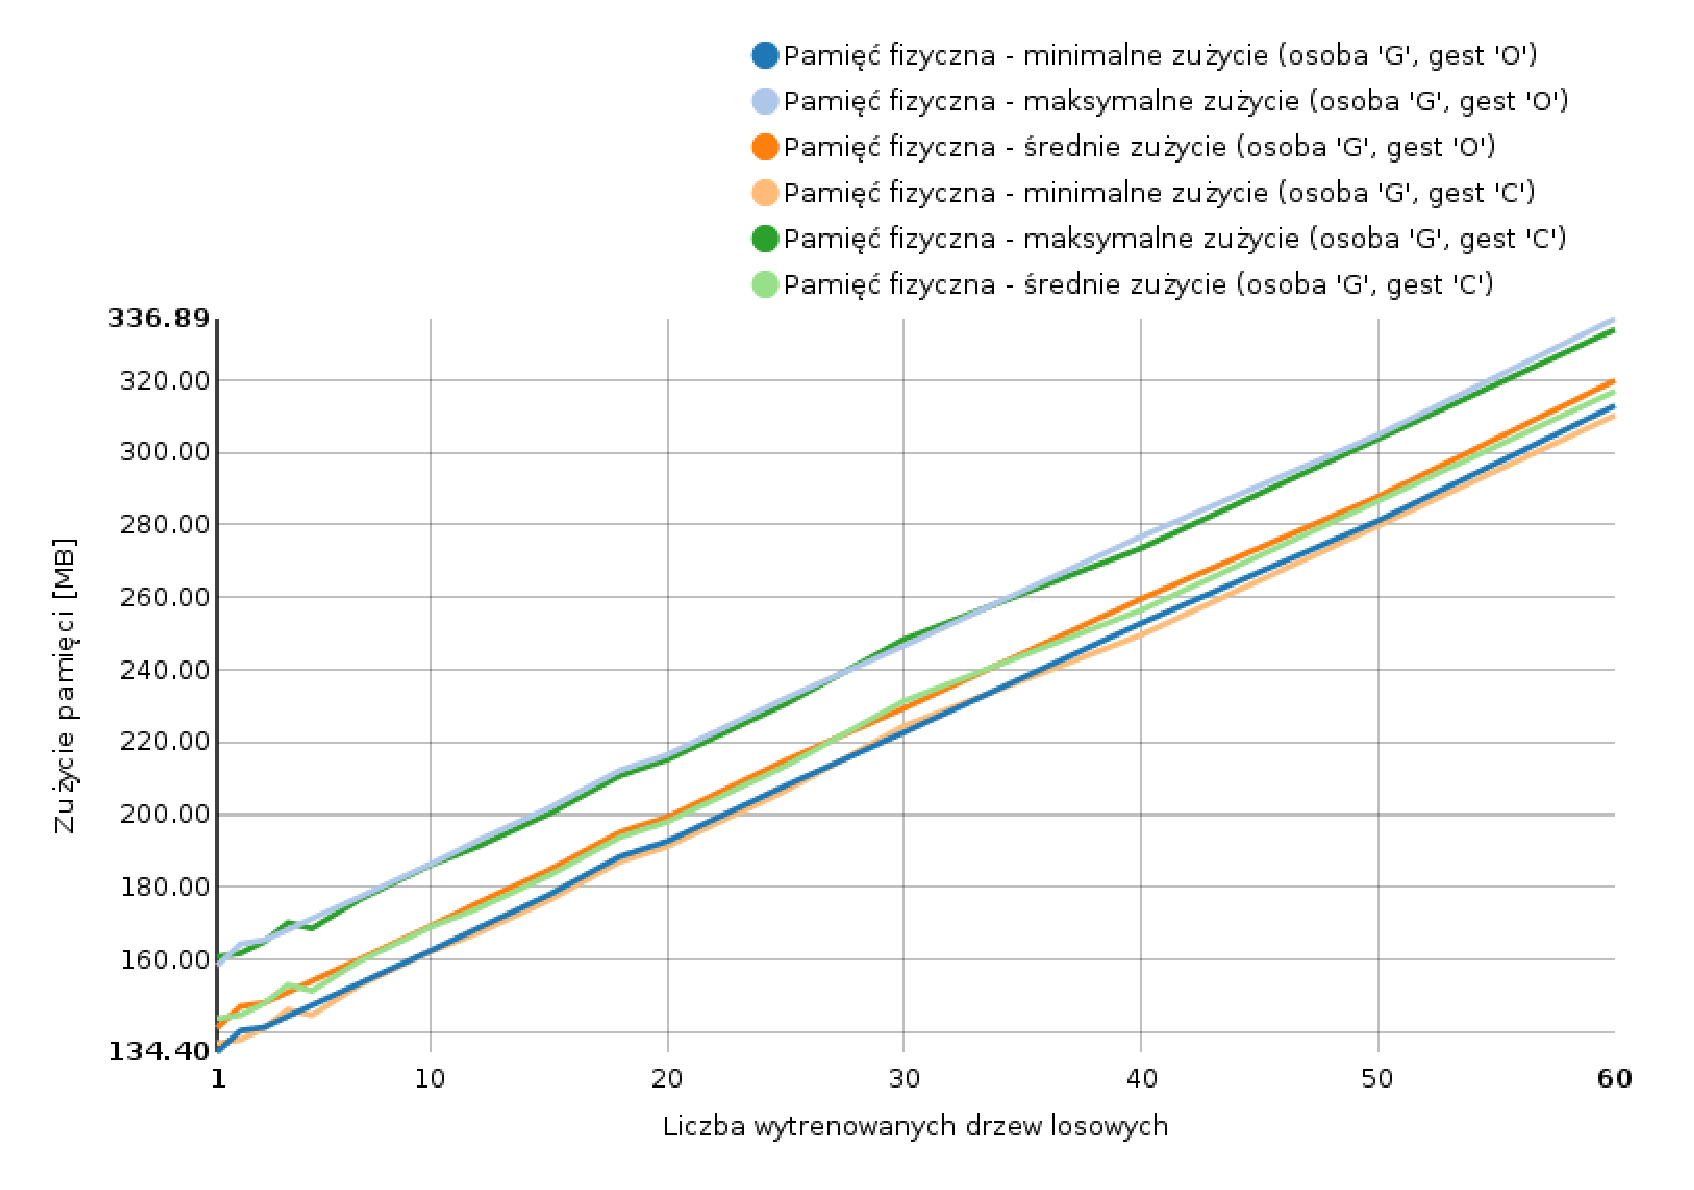
\includegraphics[width=14cm]{charts/memory/RandomPerTrainedTree}
        \caption[Wykres zużycia pamięci dla algorytmu lasu drzew losowych w~zależności od liczby wytrenowanych drzew]
                {Wykres zużycia pamięci dla algorytmu lasu drzew losowych w~zależności od liczby wytrenowanych drzew}
        \label{fig:RandomForestTrackerPerTrainedTreesAmount}
      \end{figure}

    Rzadki przepływ optyczny charakteryzuje się niewielkimi wahaniami zużycia pamięci w~zależności od minimalnej odległości pomiędzy śledzonymi punktami charakterystycznymi (jak można było przypuszczać, im większa odległość tym mniejsze zużycie pamięci). Na wykresie \ref{fig:SparseOpticalFlowPerMinimalDistanceBetweenPoints} widać, że fluktuacje mieszczą się w~przedziale o~szerokości około $30$ MB i~nie przekraczają wartości $63$ MB, co nie jest bez znaczenia w~środowisku z~ograniczonymi zasobami pamięciowymi (np. systemy wbudowane lub urządzenia mobilne). Z trzech porównywanych implementacji, metoda oparta o~algorytm \textit{LK} w~wariancie piramidalnym jest najbardziej optymalna pod względem zużycia pamięci.

      \begin{figure}[!ht]
        \centering
        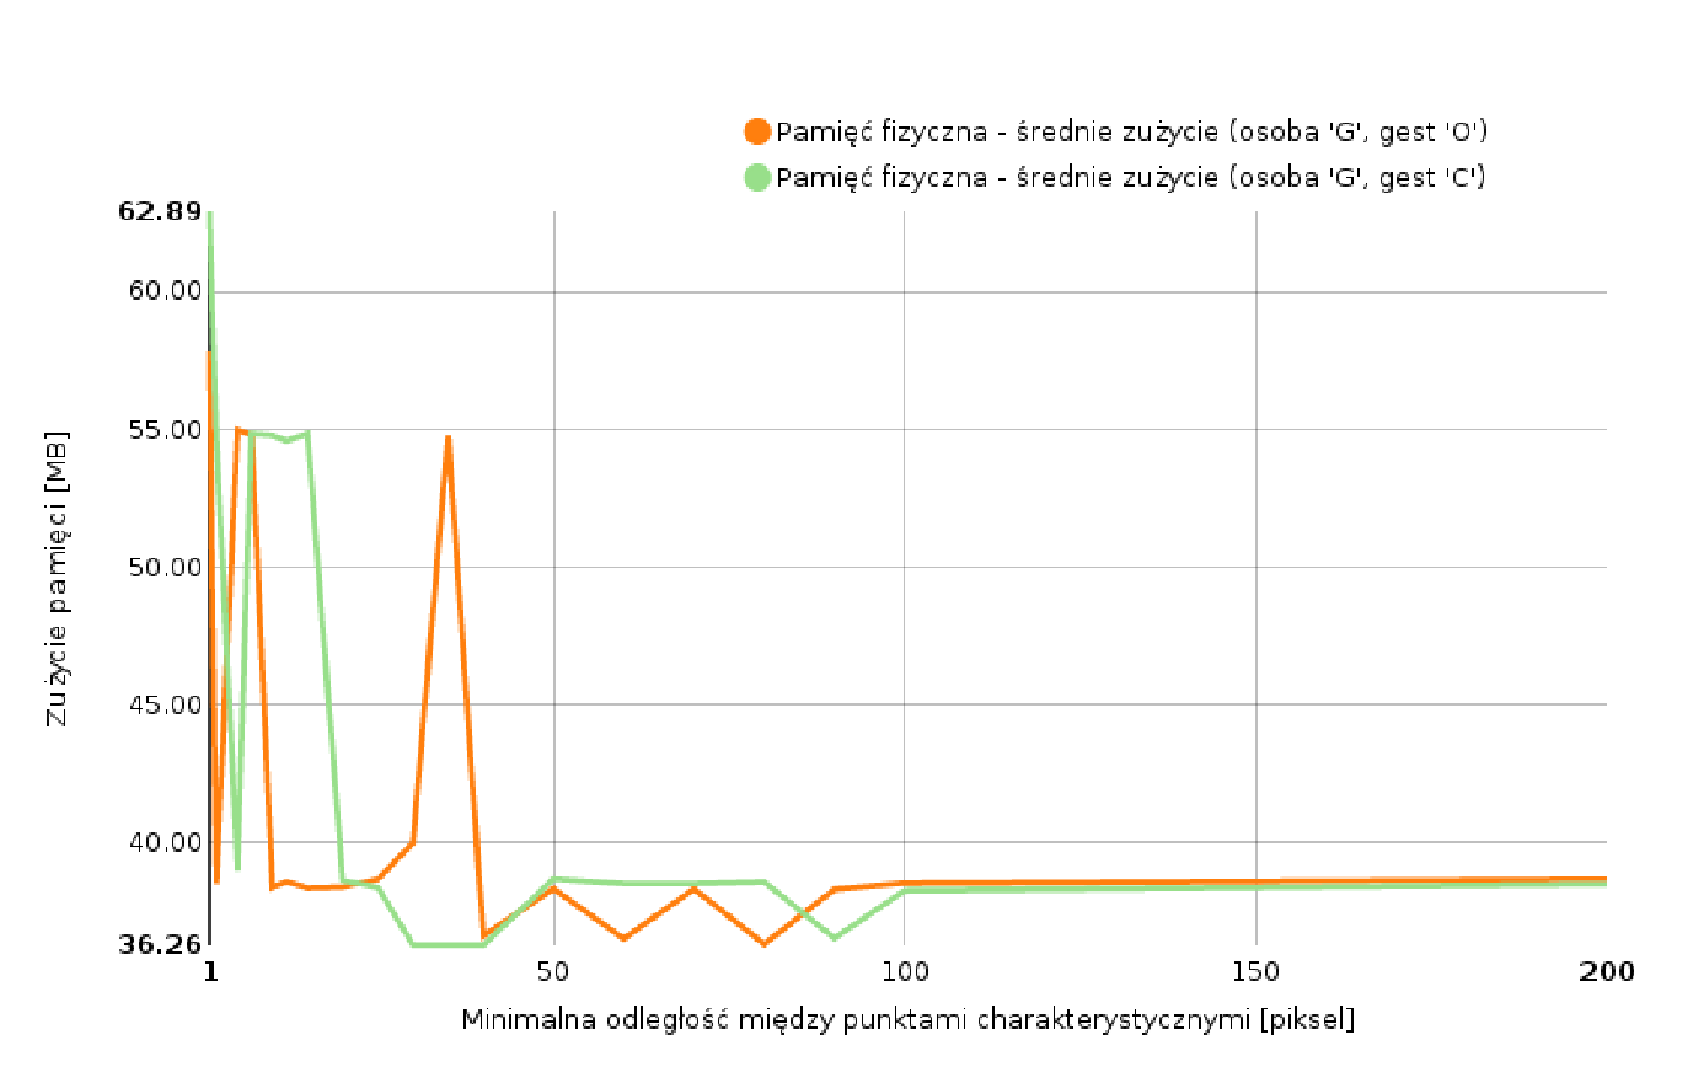
\includegraphics[width=14cm]{charts/memory/SparsePerMinimalDistance}
        \caption[Wykres zużycia pamięci dla rzadkiego przepływu optycznego w~zależności przyjętej minimalnej odległości pomiędzy punktami charakterystycznymi]
                {Wykres zużycia pamięci dla rzadkiego przepływu optycznego w~zależności przyjętej minimalnej odległości pomiędzy punktami charakterystycznymi}
        \label{fig:SparseOpticalFlowPerMinimalDistanceBetweenPoints}
      \end{figure}

      \begin{figure}[!ht]
        \centering
        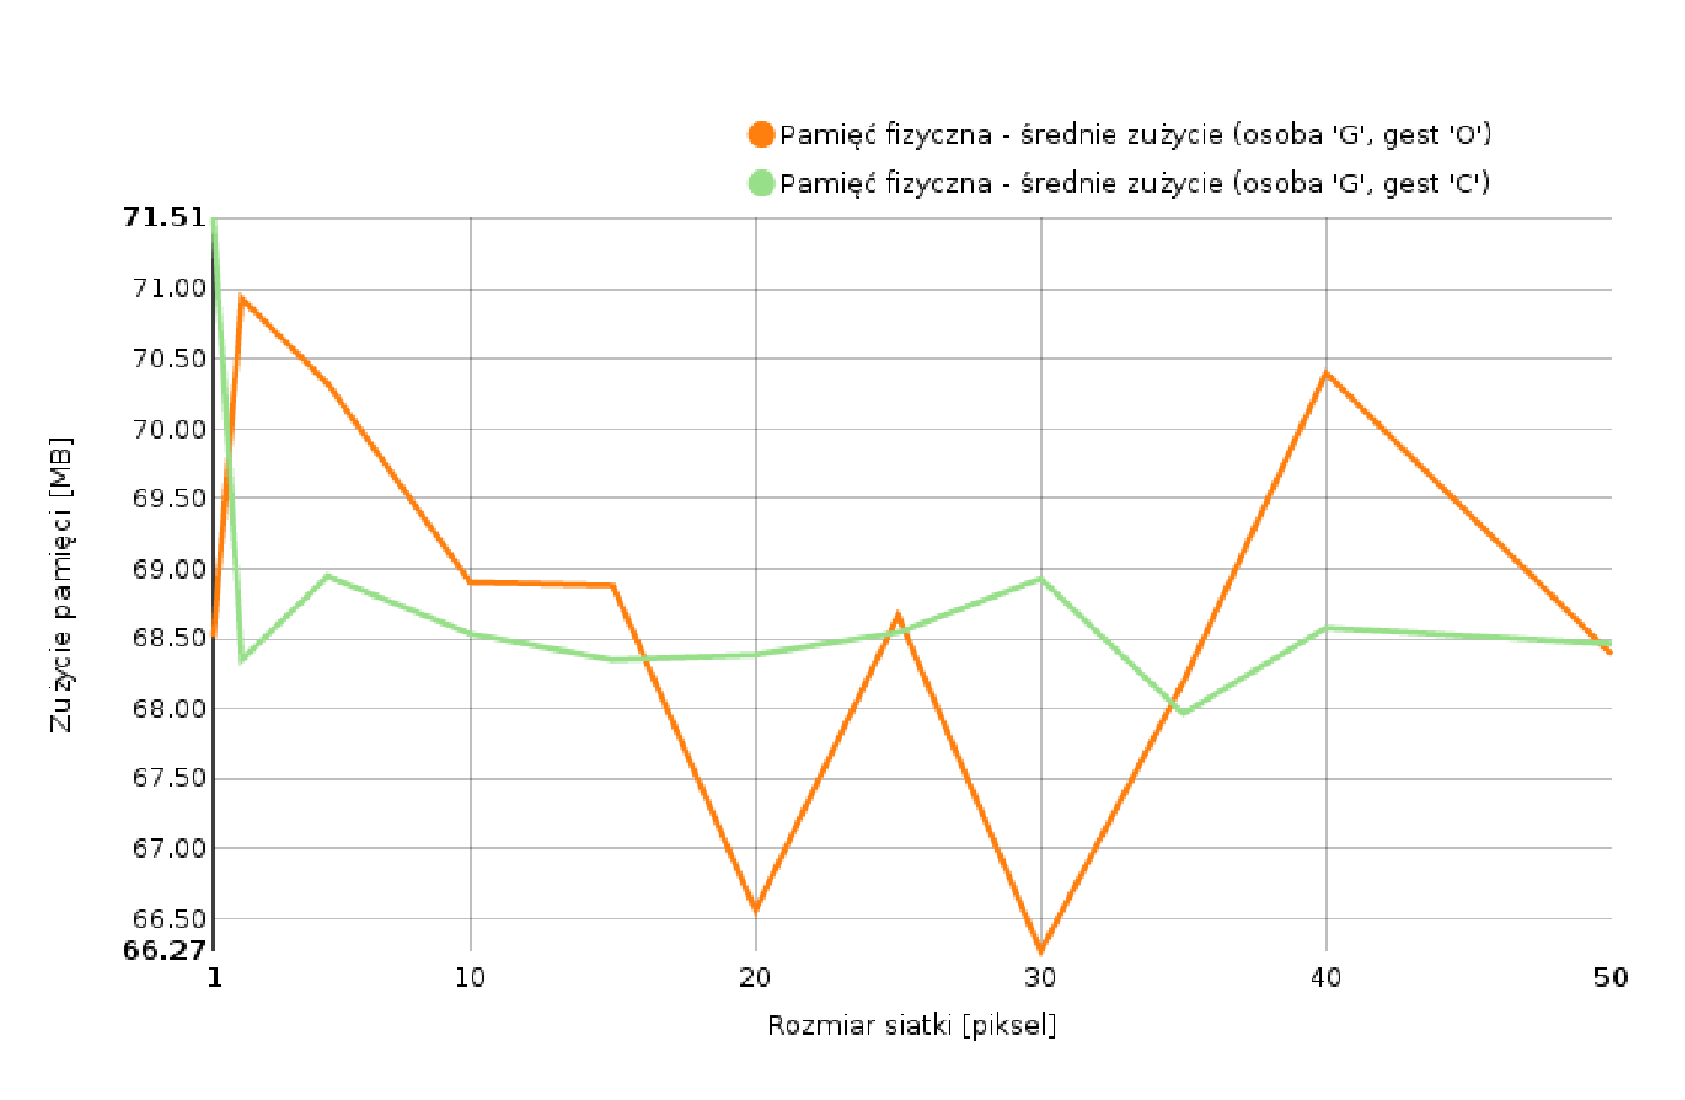
\includegraphics[width=14cm]{charts/memory/DensePerMapOverlaySize}
        \caption[Wykres zużycia pamięci dla gęstego przepływu optycznego w~zależności od gęstości siatki]
                {Wykres zużycia pamięci dla gęstego przepływu optycznego w~zależności od gęstości siatki}
        \label{fig:DenseOpticalFlowPerMapSize}
      \end{figure}

    \newpage

    W~wariancie gęstym zależnym od rozmiaru przyjętej siatki, przepływ optyczny charakteryzuje się wyższym zużyciem pamięci (maksymalnie około $72$ MB), jednak same wahania są stabilniejsze, mieszczą się w~przedziale o~szerokości około $5$ MB. Widać, że zwiększenie wymiarów siatki (intuicyjnie, rozrzedzenie jej) nie zawsze idzie w~parze z~malejącym zużyciem pamięci. Warto jednak zauważyć, że wahania odbywają się w~bardzo niewielkim zakresie.

    Mimo wyższego zużycia całościowego, jego wartość nadal nie jest zbyt wysoka i~algorytm gęstego przepływu optycznego sprawdzi się w~środowisku z~ograniczonymi zasobami pamięciowymi.

  \section{Wydajność badanych algorytmów}\label{Section_Timing}

    Pod pojęciem badań wydajności zostały zebrane wszystkie testy oraz wykresy prezentujące czas przetwarzania pojedynczej klatki algorytmu. Wszystkie implementacje zostały szczegółowo zbadane pod tym kątem, aby wybrać algorytm najefektywniejszy i~dokładający najmniejszy narzut w~każdej kolejnej klatce sekwencji wideo.

    Na wykresach \ref{fig:DenseTimingPersonAC}, \ref{fig:RandomTimingPersonAC} oraz \ref{fig:SparseTimingPersonAC} widać wartości czasu przetwarzania klatki, wraz z~naniesioną wartością średnią dla zaimplementowanych algorytmów kolejno przepływu w~wariancie gęstym, wykorzystującym lasy drzew losowych oraz rzadkiego przepływu optycznego.

      \begin{figure}[!ht]
        \centering
        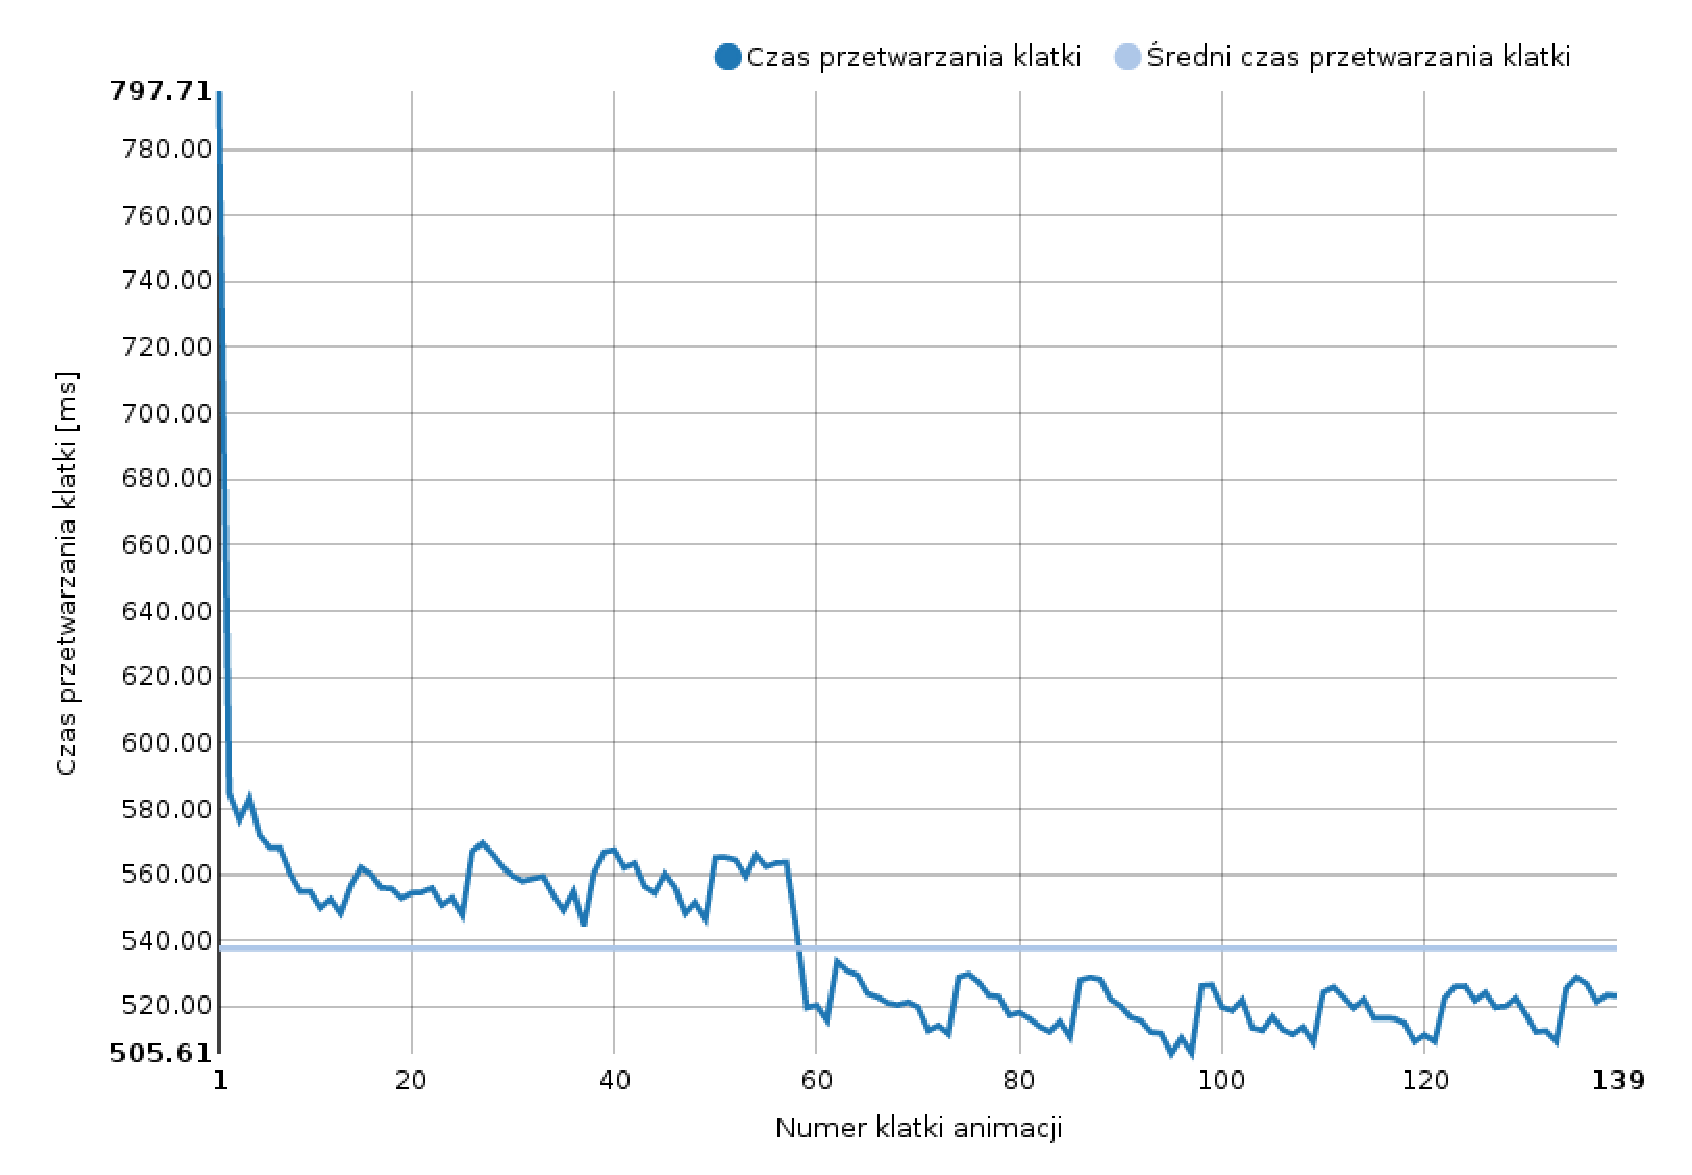
\includegraphics[width=14cm]{charts/timing/DenseTimingPersonAC}
        \caption[Wykres czasu przetwarzania klatki dla algorytmu gęstego przepływu optycznego]
                {Wykres czasu przetwarzania klatki dla algorytmu gęstego przepływu optycznego}
        \label{fig:DenseTimingPersonAC}
      \end{figure}

    \newpage
      \begin{figure}[!ht]
        \centering
        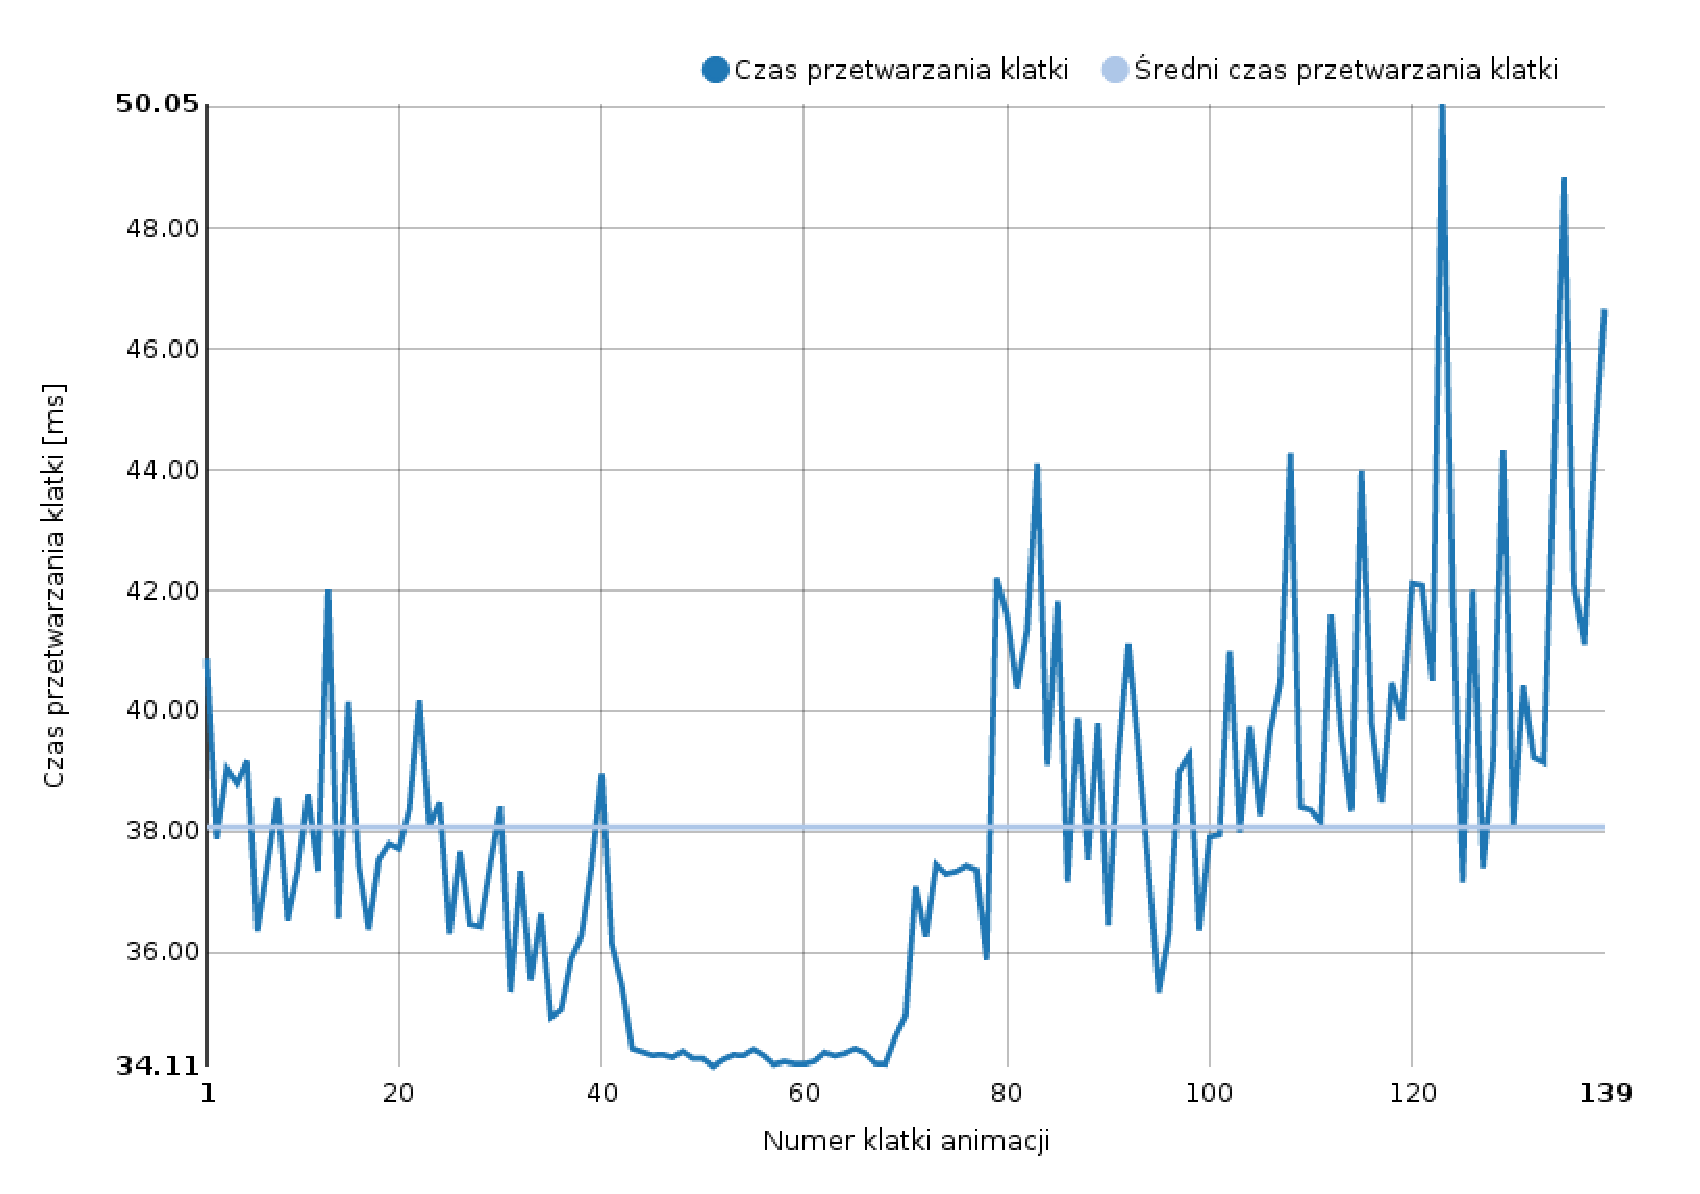
\includegraphics[width=12cm]{charts/timing/RandomTimingPersonAC}
        \caption[Wykres czasu przetwarzania klatki dla algorytmu lasu drzew losowych]
                {Wykres czasu przetwarzania klatki dla algorytmu lasu drzew losowych}
        \label{fig:RandomTimingPersonAC}
      \end{figure}

      \begin{figure}[!ht]
        \centering
        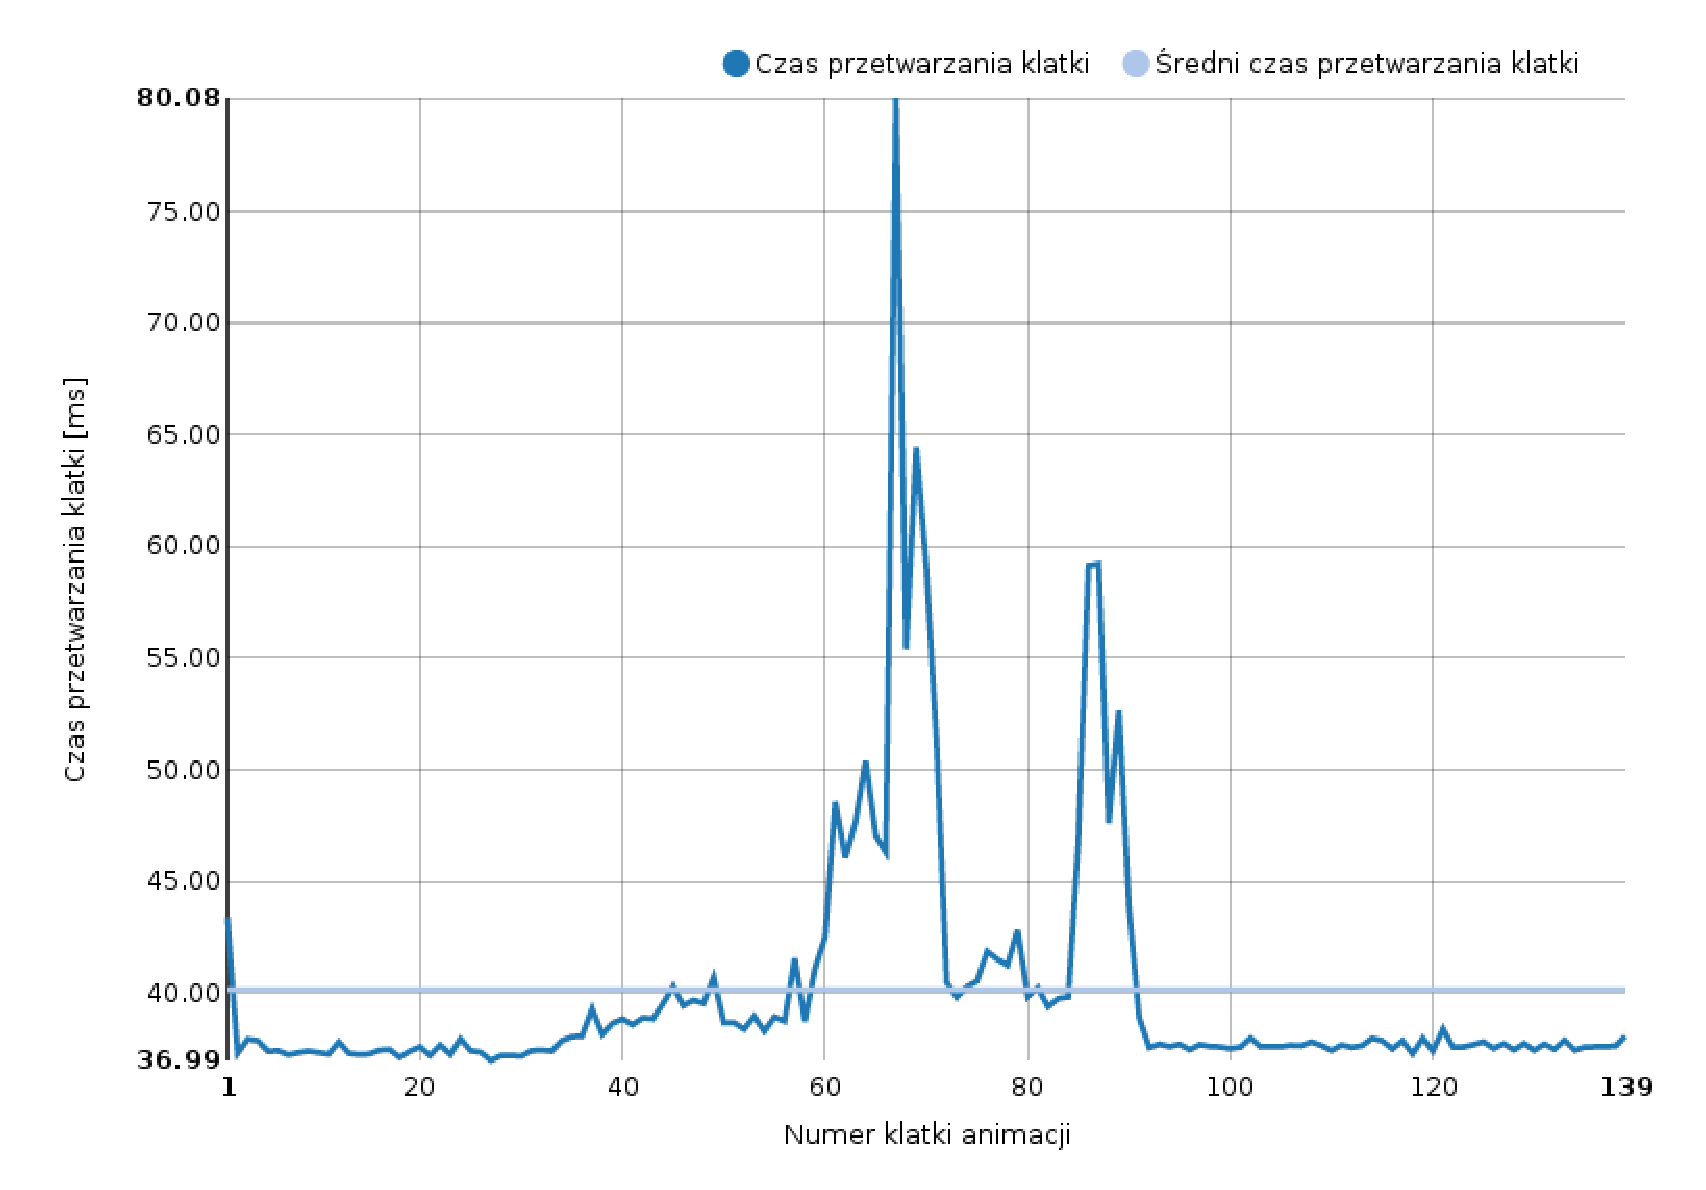
\includegraphics[width=12cm]{charts/timing/SparseTimingPersonAC}
        \caption[Wykres czasu przetwarzania klatki dla algorytmu rzadkiego przepływu optycznego]
                {Wykres czasu przetwarzania klatki dla algorytmu rzadkiego przepływu optycznego}
        \label{fig:SparseTimingPersonAC}
      \end{figure}

    Widać, że najmniejszym średnim czasem przetwarzania charakteryzują się dwa ostatnie algorytmu. Gęsty przepływ optyczny jest algorytmem o~bardzo dużym koszcie obliczeniowym, co objawia się bardzo wysokimi wartościami czasu przetwarzania klatki (oraz w~konsekwencji dużo wyższą wartością średnią). Zależność tą najlepiej widać na wykresach \ref{fig:PersonBO} oraz \ref{fig:PersonGO}.

      \begin{figure}[!ht]
        \centering
        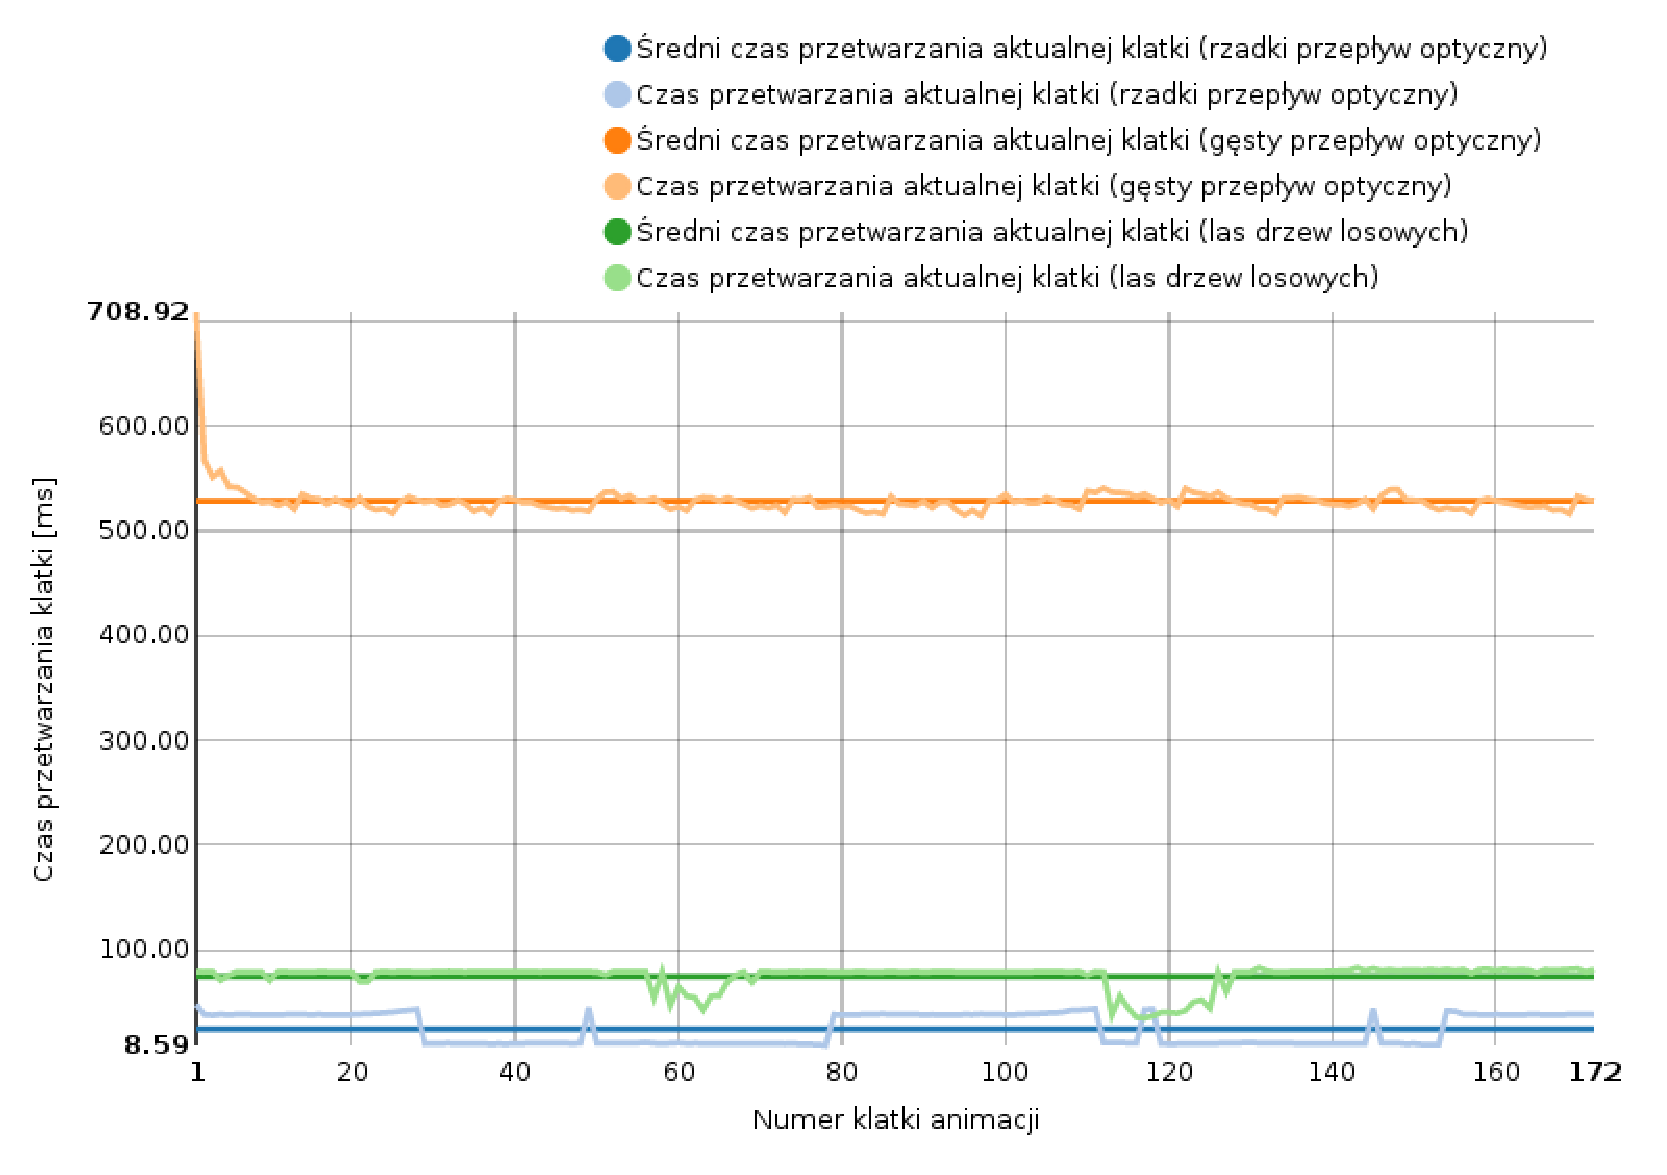
\includegraphics[width=14cm]{charts/timing/PersonBO}
        \caption[Porównanie czasu przetwarzania klatki dla próbki Person\_B\_O]
                {Porównanie czasu przetwarzania klatki dla próbki \textit{Person\_B\_O}}
        \label{fig:PersonBO}
      \end{figure}

      \begin{figure}[!ht]
        \centering
        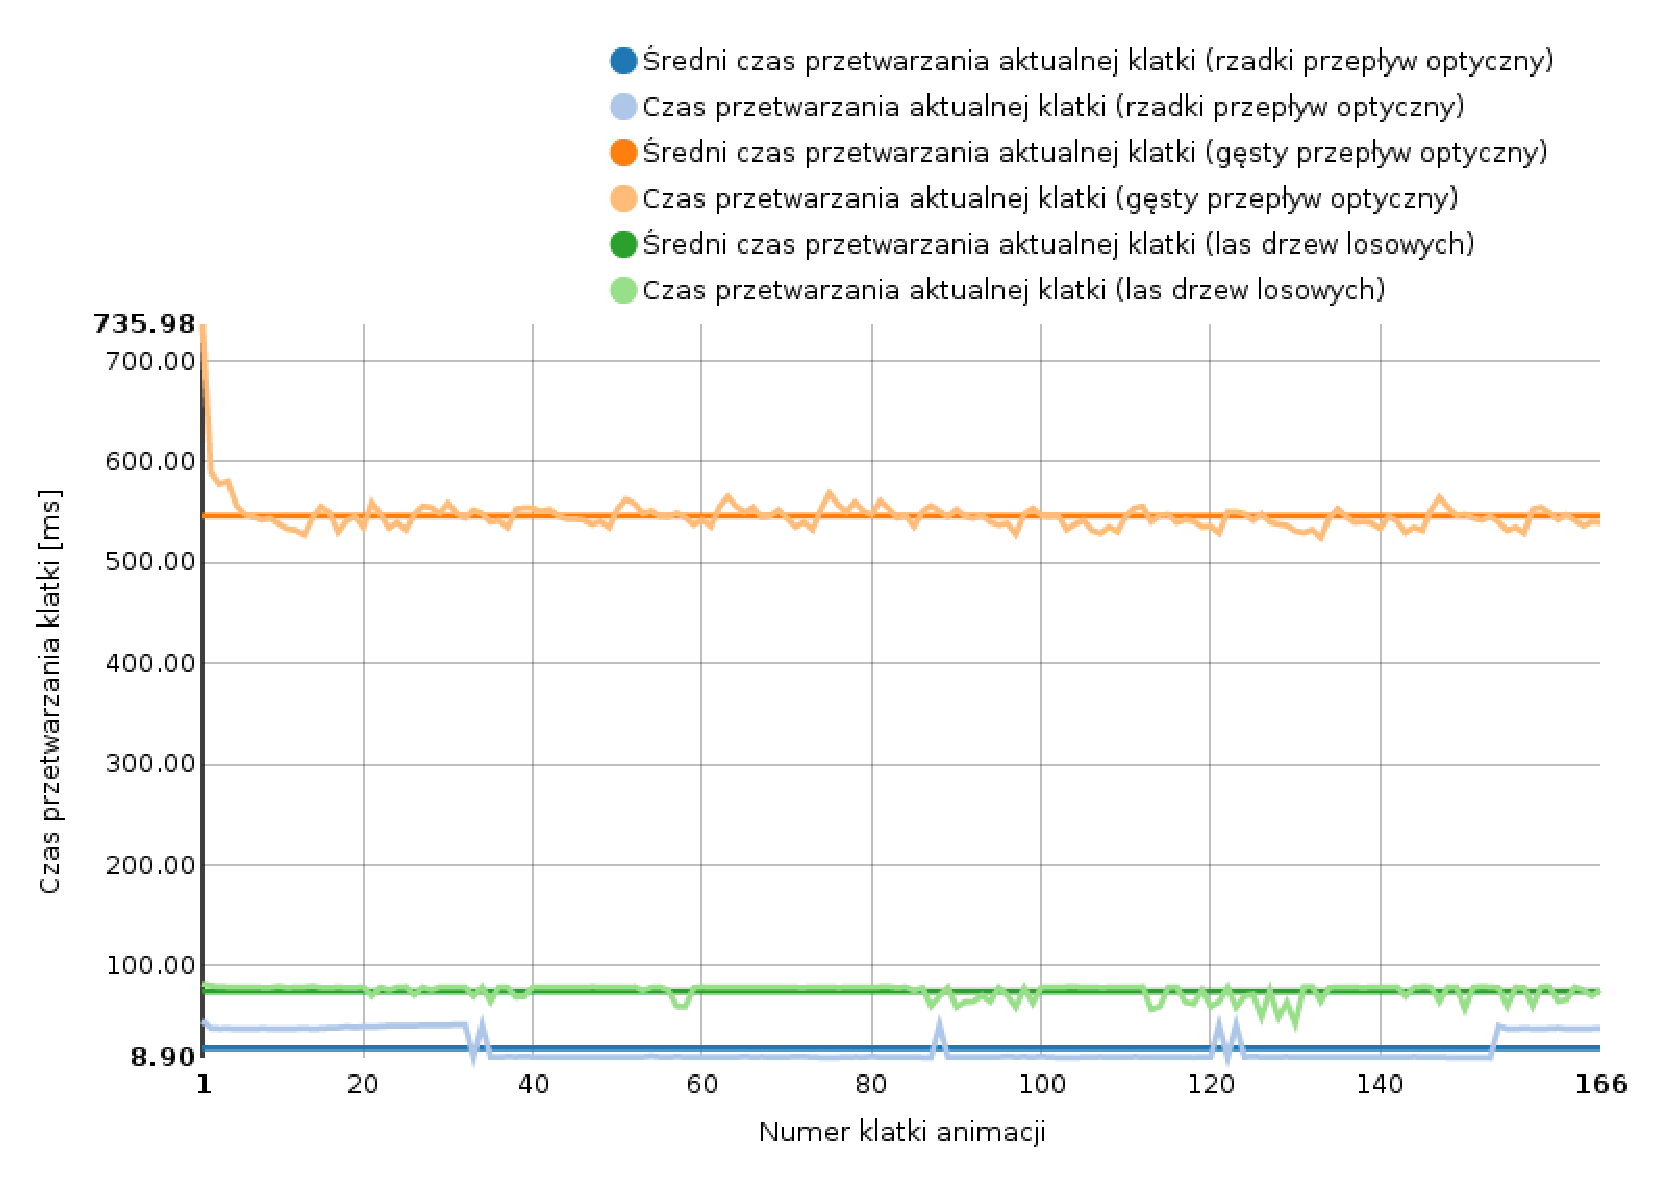
\includegraphics[width=14cm]{charts/timing/PersonGO}
        \caption[Porównanie czasu przetwarzania klatki dla próbki Person\_G\_O]
                {Porównanie czasu przetwarzania klatki dla próbki \textit{Person\_G\_O}}
        \label{fig:PersonGO}
      \end{figure}

    Warto zauważyć, że praktycznie każdy z~algorytmów charakteryzuje się niewielkimi wahaniami w~zakresie czasu przetwarzania (wyjątkiem jest początkowa faza działania algorytmu gęstego przepływu optycznego, gdzie następuje inicjalizacja macierzy przepływu, w~kolejnym etapie czas przetwarzania stabilizuje się).

      \begin{figure}[!ht]
        \centering
        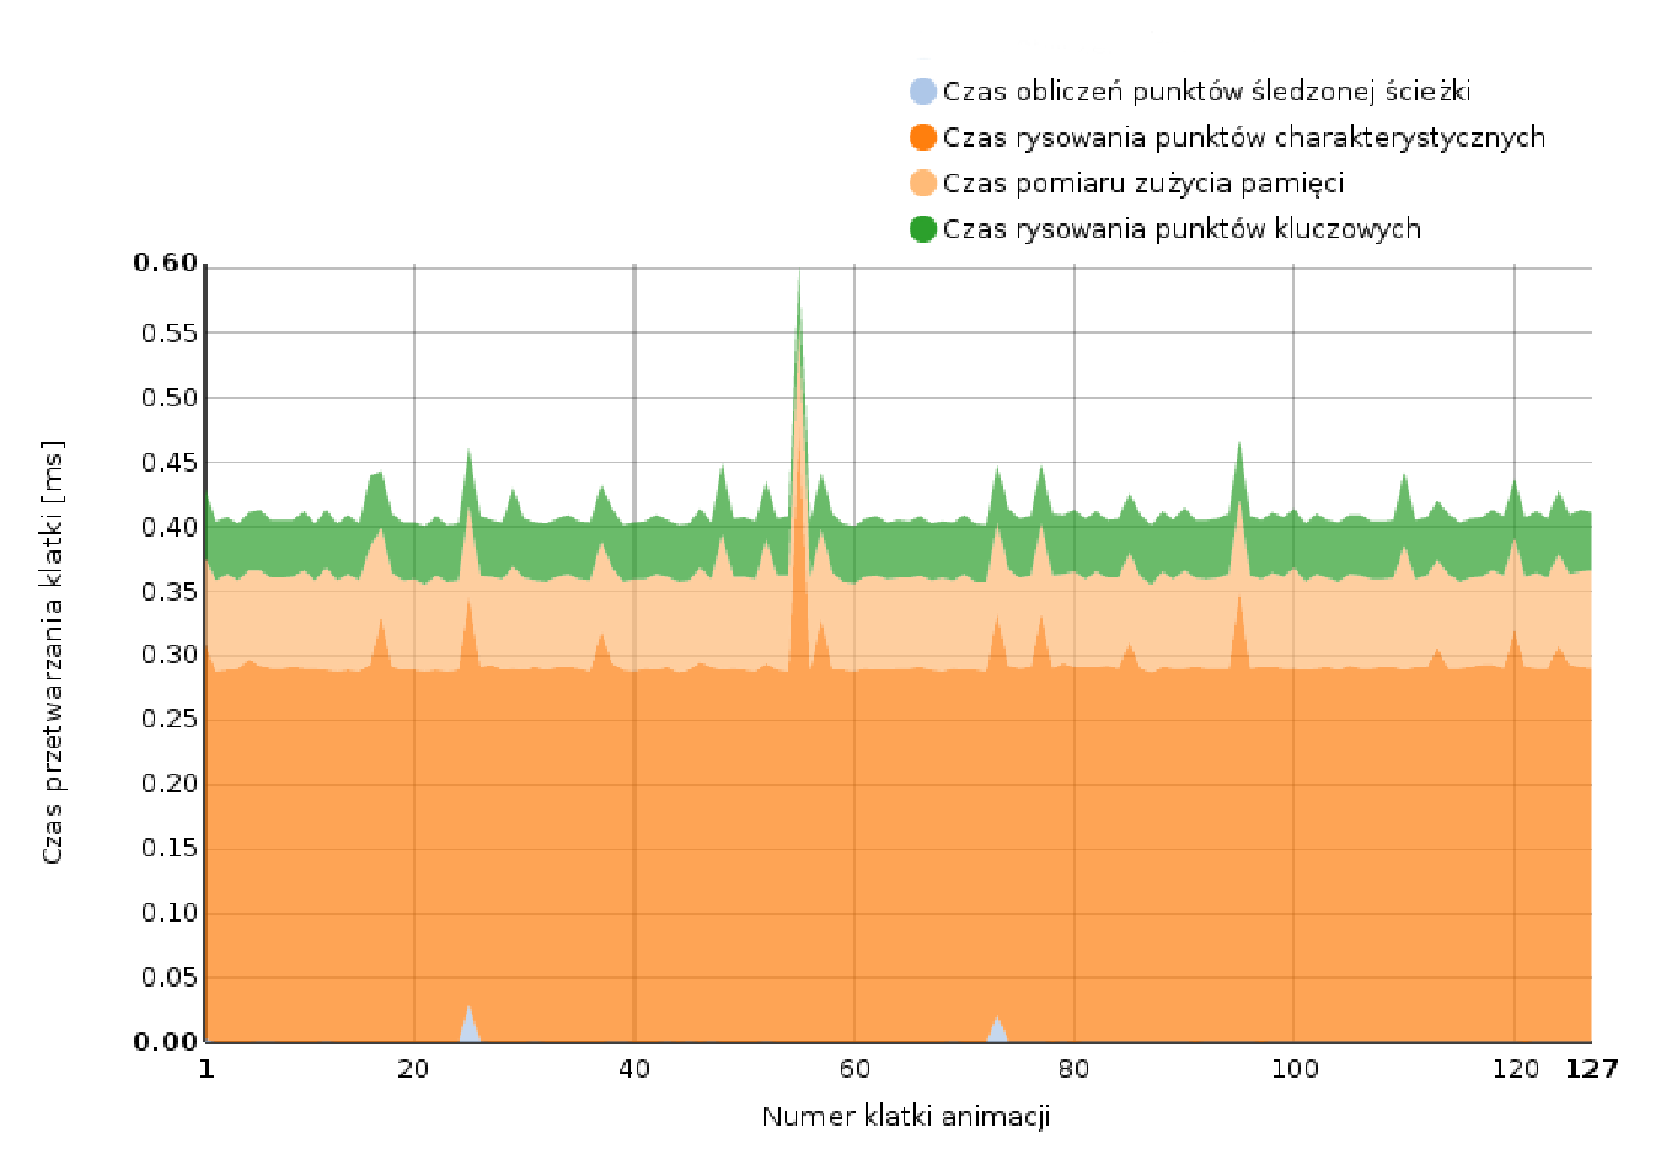
\includegraphics[width=10cm]{charts/timing/StackedDensePersonEGestureCrush}
        \caption[Narzut czasowy dodatkowych etapów przetwarzania dla każdej klatki\\(gęsty przepływ optyczny)]
                {Narzut czasowy dodatkowych etapów przetwarzania dla każdej klatki\\(gęsty przepływ optyczny)}
        \label{fig:StackedDense}
      \end{figure}

      \begin{figure}[!ht]
        \centering
        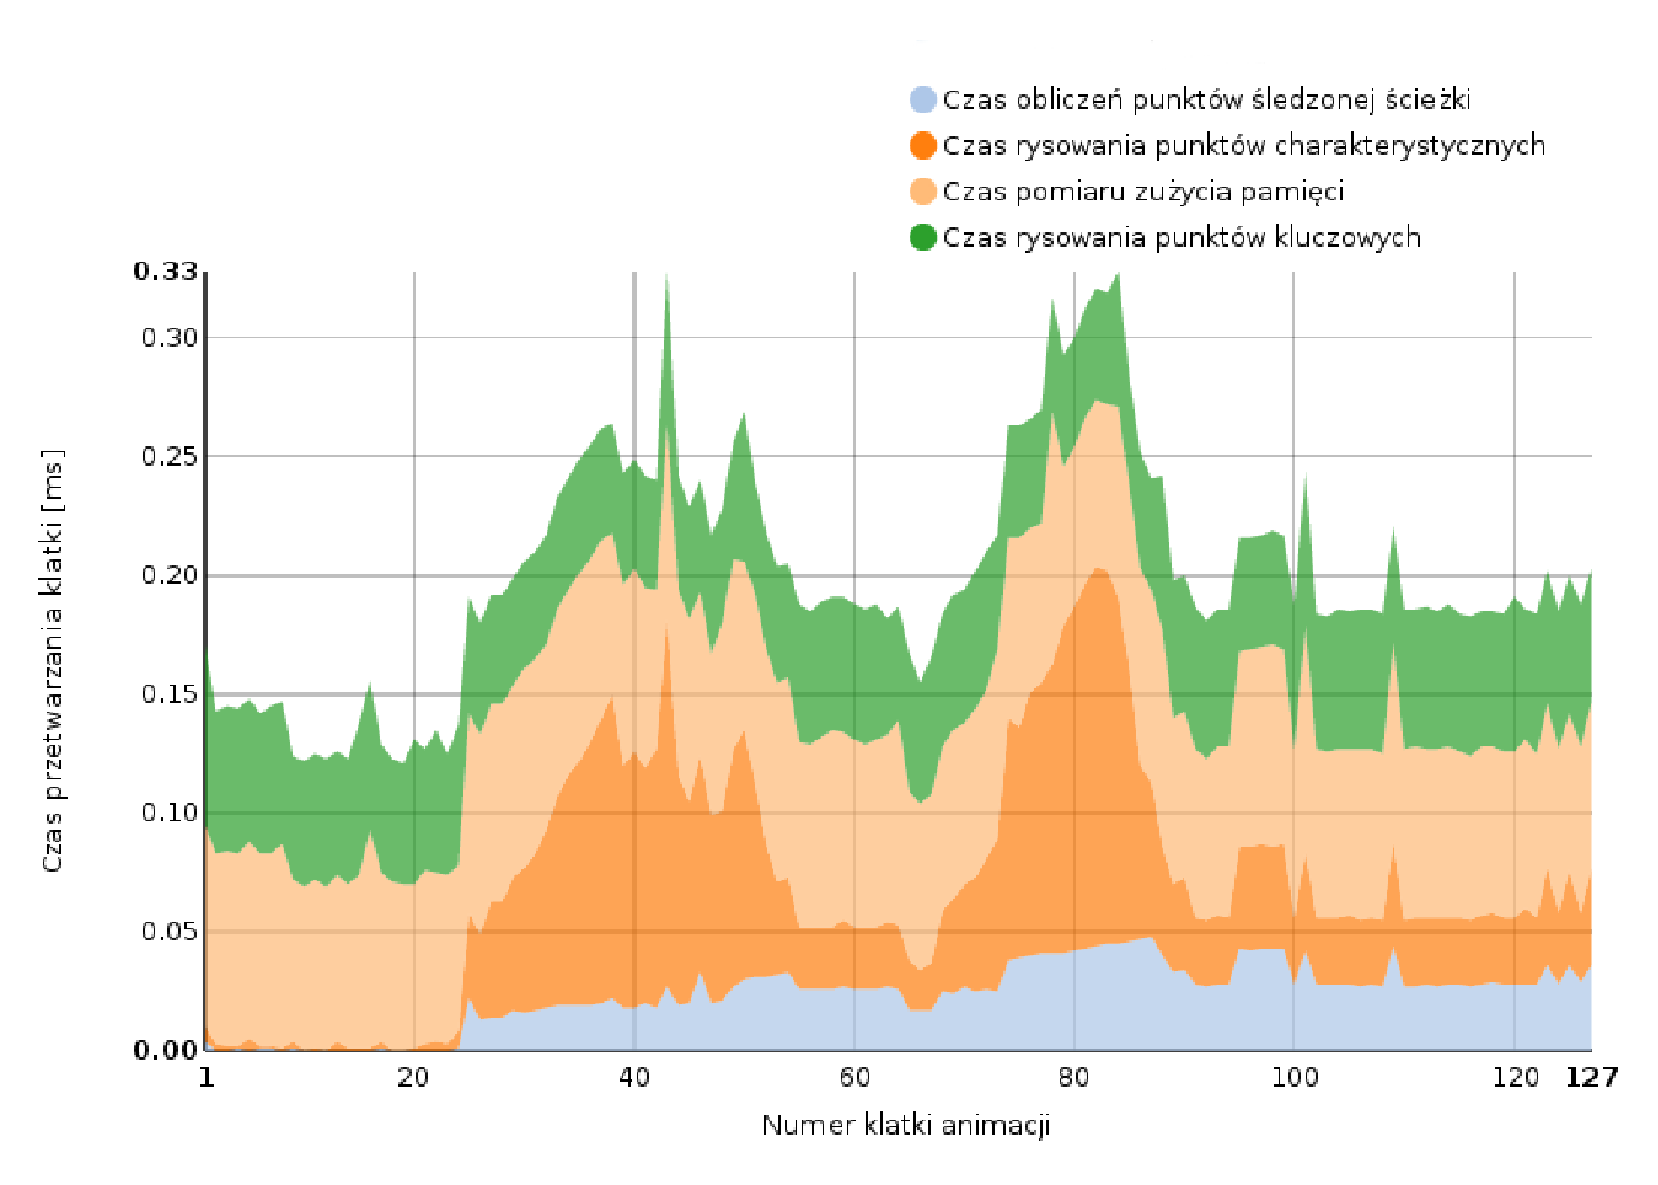
\includegraphics[width=10cm]{charts/timing/StackedSparsePersonEGestureCrush}
        \caption[Narzut czasowy dodatkowych etapów przetwarzania dla każdej klatki\\(rzadki przepływ optyczny)]
                {Narzut czasowy dodatkowych etapów przetwarzania dla każdej klatki\\(rzadki przepływ optyczny)}
        \label{fig:StackedSparse}
      \end{figure}

    \newpage
      \begin{figure}[!ht]
        \centering
        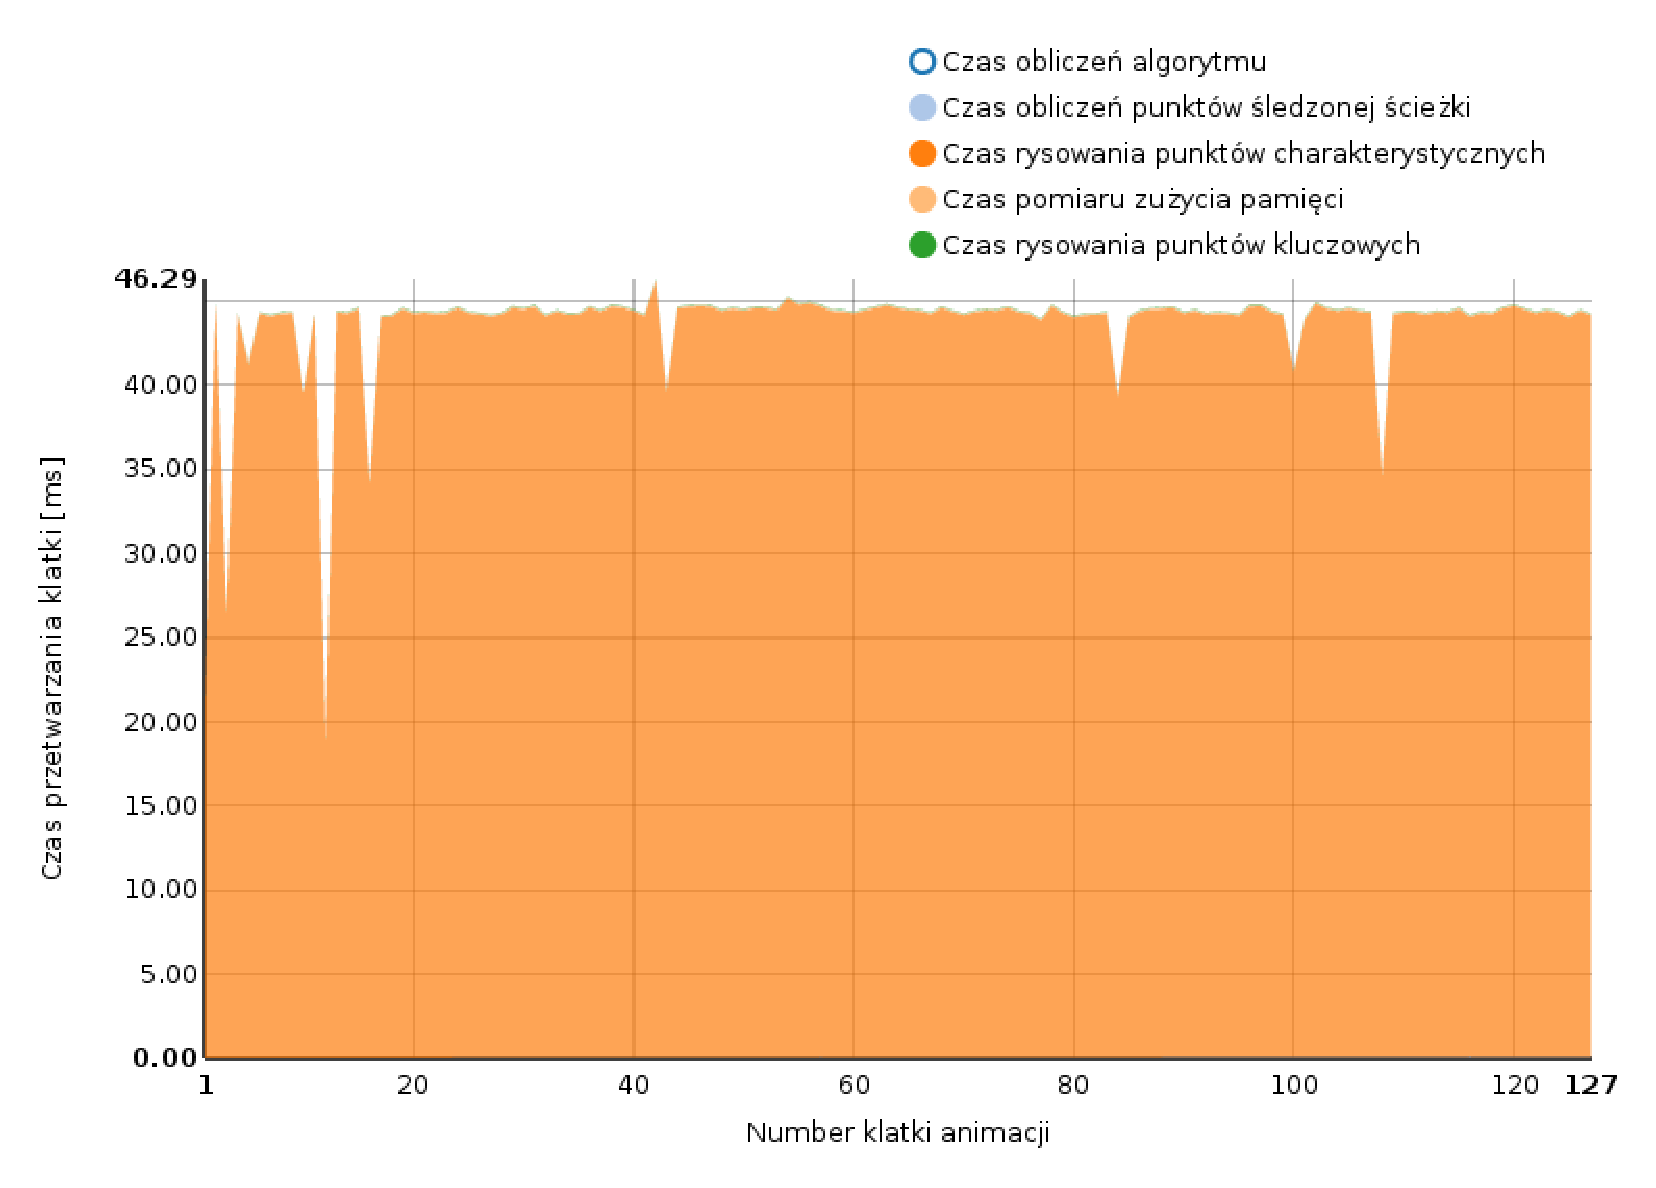
\includegraphics[width=12cm]{charts/timing/StackedRandomPersonEGestureCrush}
        \caption[Narzut czasowy dodatkowych etapów przetwarzania dla każdej klatki\\(las drzew losowych)]
                {Narzut czasowy dodatkowych etapów przetwarzania dla każdej klatki\\(las drzew losowych)}
        \label{fig:StackedRandom}
      \end{figure}

    Reprezentacja graficzna narzutu dodatkowych etapów przetwarzania została zamieszczona na wykresach \ref{fig:StackedDense}, \ref{fig:StackedSparse} oraz \ref{fig:StackedRandom}. Widać wyraźnie, że w~przypadku algorytmów z~rodziny przepływu optycznego dodatkowy narzut mieści się w~granicy błędu statystycznego (maksymalne wartości odpowiednio $0.6$ oraz $0.33$ milisekundy).

    W~przypadku algorytmu opartego o~uczenie maszynowe, odzyskanie reprezentacji śledzonych punktów wiąże się z~niewielkim narzutem czasowym, odzwierciedlonym na przebiegu \ref{fig:StackedRandom} (maksymalnie ok. $50$ milisekund).

    Dla algorytmu gęstego przepływu optycznego najcięższą przeprawą jeśli chodzi o~przetwarzanie okazał się zestaw próbek \textit{G}, choć tak naprawdę czasy przetwarzania wszystkich zbiorów mieszczą się w~przedziale o~dość niewielkiej szerokości (jeśli chodzi o~średnie czas przetwarzania, przedział ma szerokość około $20$ milisekund). Omawiana implementacja charakteryzuje się bardzo stabilnym czasem przetwarzania pojedynczej klatki. Niemniej, jest to zbyt duża wartość, aby można było mówić o~zastosowaniu tej metody w~przypadku ścisłych wymagań czasowych.

    Tak jak w~przypadku zbiorów, również podział ze względu na gesty dla wybranej próbki charakteryzuje się stabilnym czasem przetwarzania. Różnice pomiędzy średnimi wartościami są niewielkie (szerokość przedziału to około 25 milisekund).

      \begin{figure}[!ht]
        \centering
        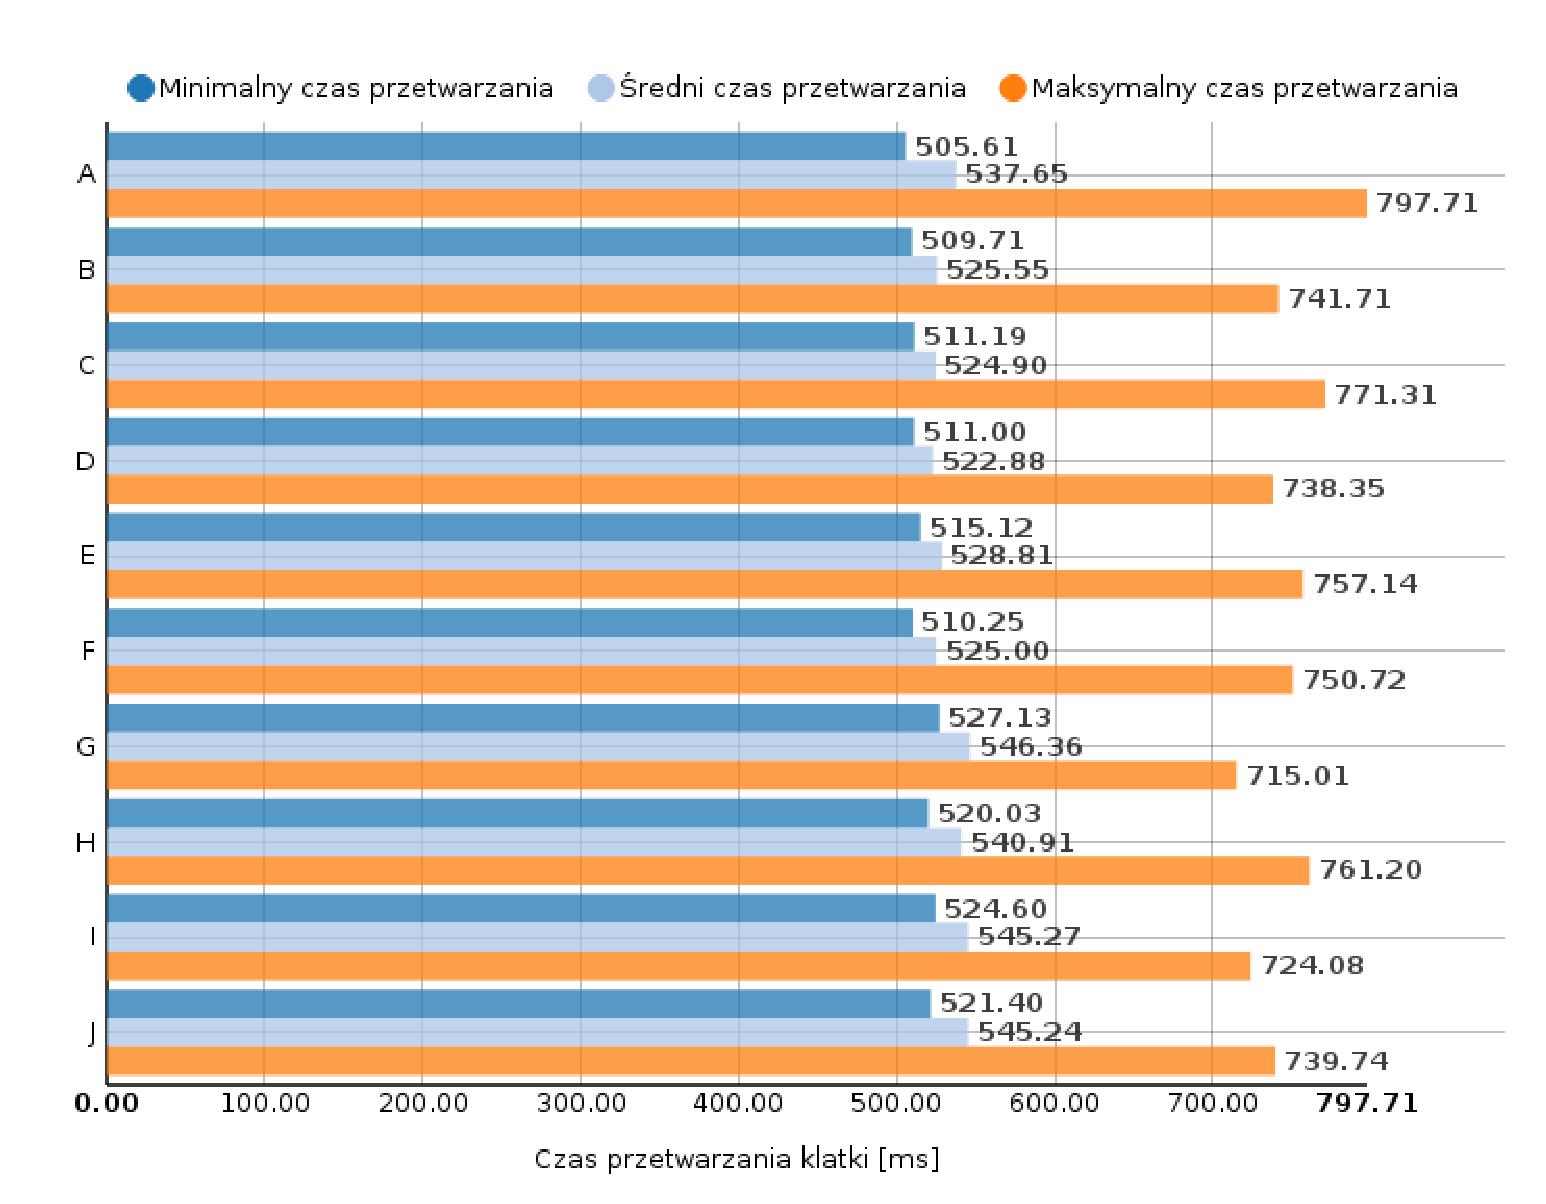
\includegraphics[width=12cm]{charts/timing/DenseForGestureC}
        \caption[Czas przetwarzania klatki każdej osoby dla gestu C (gęsty przepływ optyczny)]
                {Czas przetwarzania klatki każdej osoby dla gestu \\\textit{Wielka Litera C} (gęsty przepływ optyczny)}
        \label{fig:DenseForGestureC}
      \end{figure}

      \begin{figure}[!ht]
        \centering
        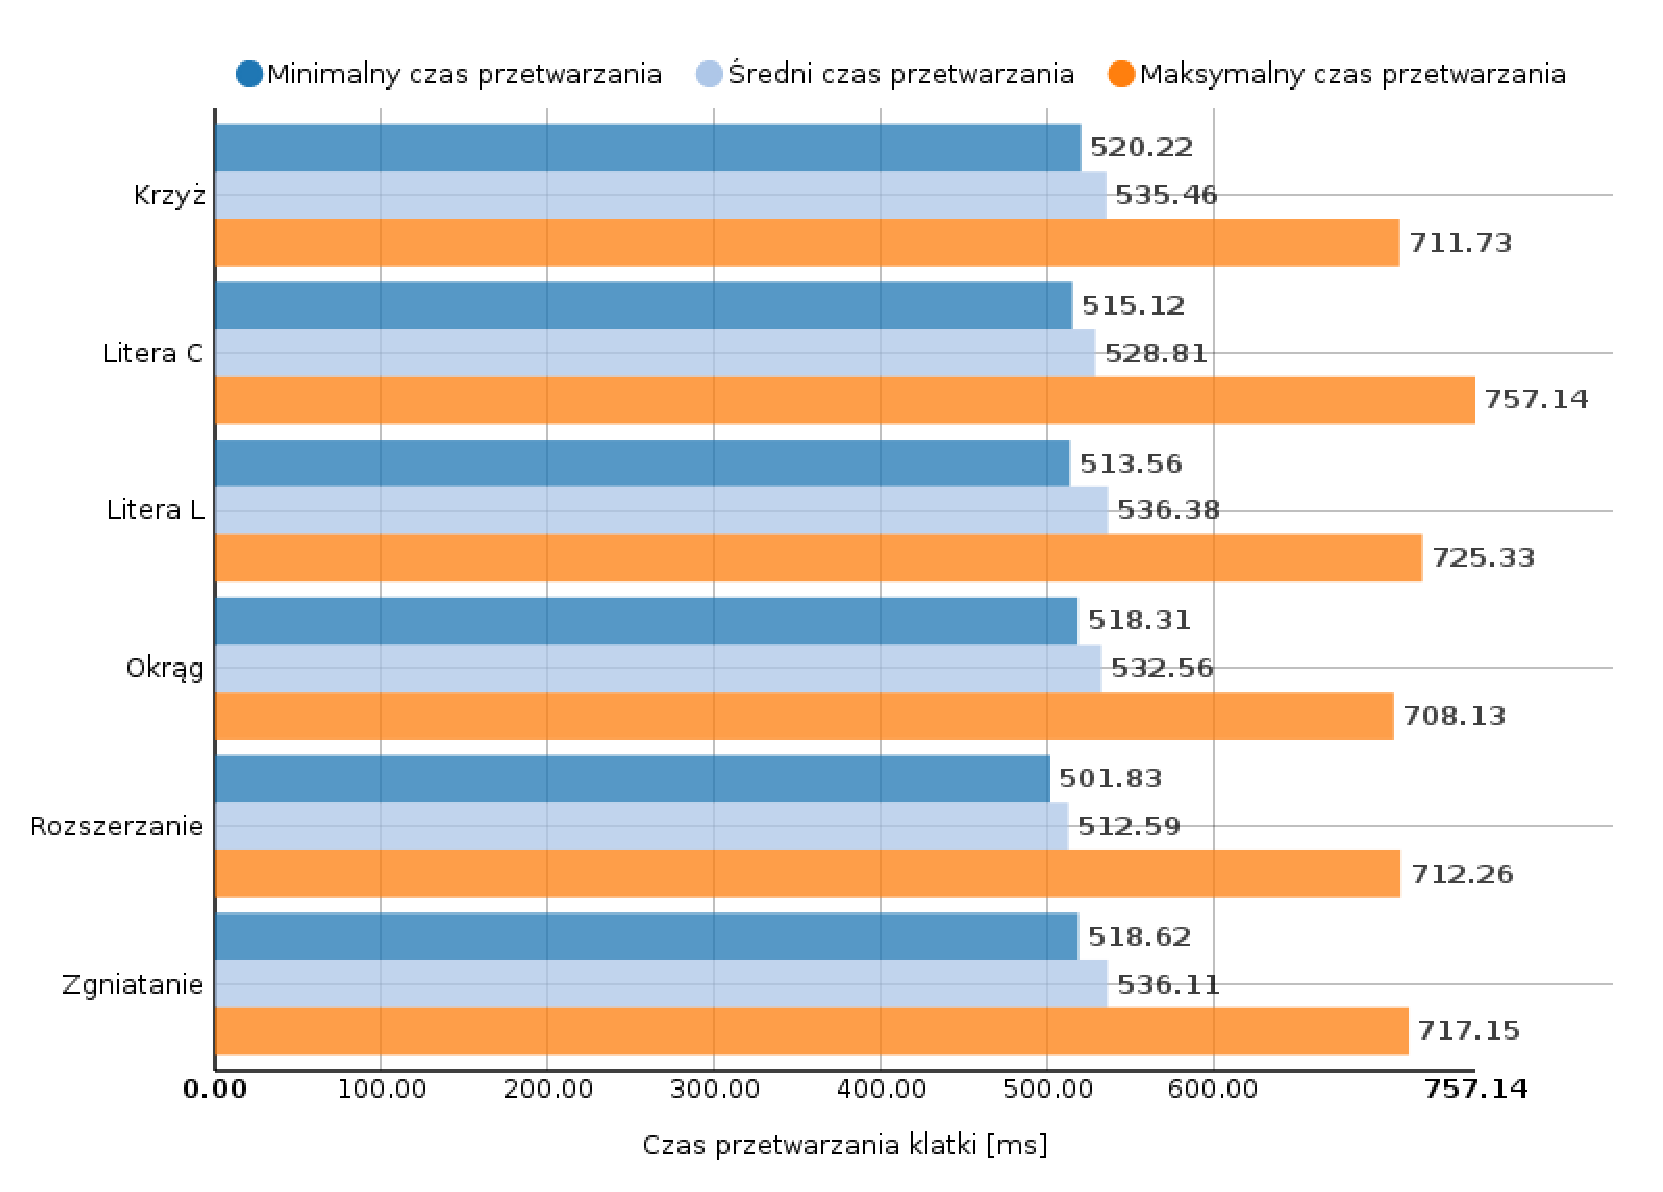
\includegraphics[width=13cm]{charts/timing/DenseTimingForPersonE}
        \caption[Czas przetwarzania klatki każdego gestu dla osoby E (gęsty przepływ optyczny)]
                {Czas przetwarzania klatki każdego gestu dla osoby \textit{E}\\(gęsty przepływ optyczny)}
        \label{fig:DenseTimingForPersonE}
      \end{figure}

    \newpage
    Na wykresie \ref{fig:DenseTimingPerMapSize} została przedstawiona zależność czasu przetwarzania od rozmiaru siatki. Intuicyjnie dla małych wartości wraz z~rozrzedzaniem gęstości siatki maleje czas przetwarzania. Po osiągnięciu pewnego pułapu (w~okolicach 10 pikseli) czas przetwarzania stabilizuje się na wcześniej obserwowanej wartości.

      \begin{figure}[!ht]
        \centering
        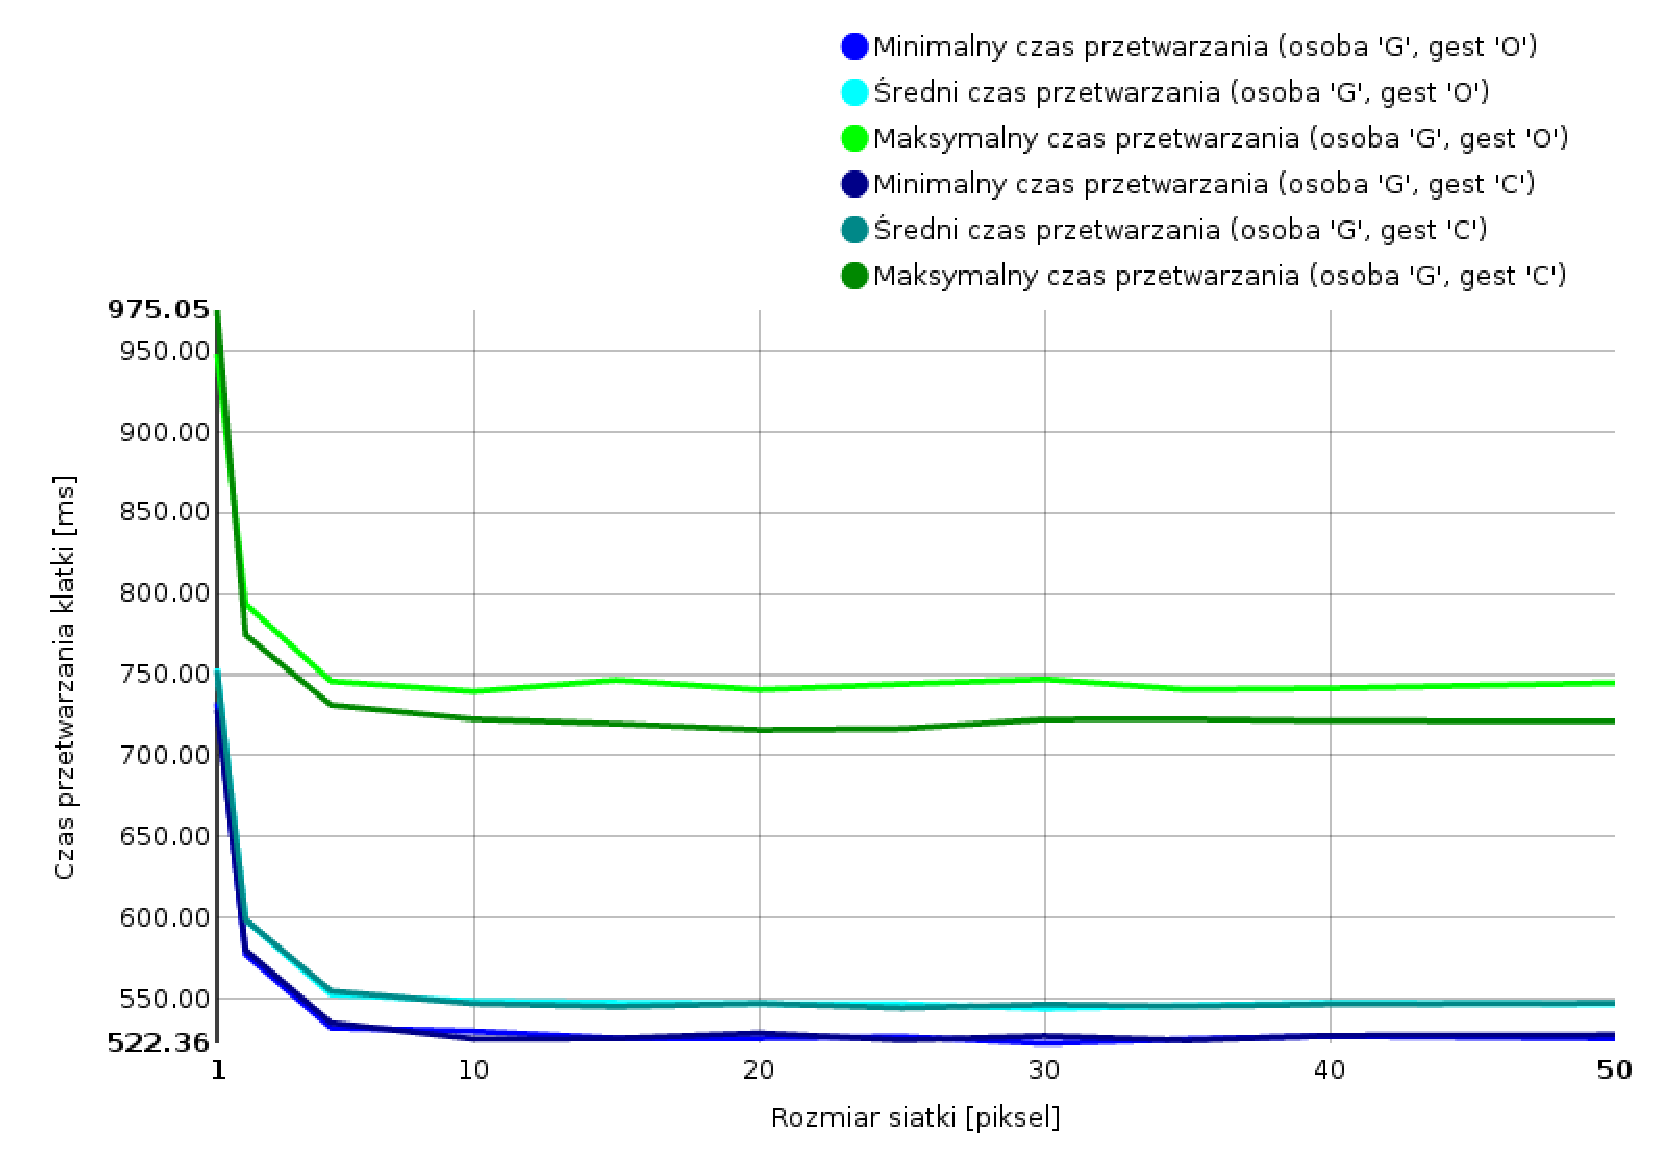
\includegraphics[width=14cm]{charts/timing/DenseTimingPersonG_OC_perMapSize}
        \caption[Czas przetwarzania klatki w~zależności od rozmiaru siatki]
                {Czas przetwarzania klatki w~zależności od rozmiaru siatki\\(próbki \textit{Person\_G\_O} oraz \textit{Person\_G\_C})}
        \label{fig:DenseTimingPerMapSize}
      \end{figure}

    Analogiczny zestaw testów został przeprowadzony na algorytmie wykorzystującym las drzew losowych.

    W~jego przypadku największym wyzwaniem okazał się zbiór \textit{B} (rysunek \ref{fig:RandomForGestureC}). Warto zwrócić na stosunkowo niski średni czas przetwarzania w~porównaniu do uprzednio omawianego algorytmu. W~przypadku podziału na gesty, wartości minimalne, maksymalne oraz średnie są zbliżone do poprzedniej reprezentacji (wykres \ref{fig:RandomTimingForPersonE}). Algorytm charakteryzuje się niskim i~dość stabilnym średnim czasem przetwarzania klatki sekwencji wideo.

    W~przypadku tej konkretnej implementacji bardzo ważnym parametrem jest czas uczenia klasyfikatora przedstawiony w~zależności od liczby wykorzystanych drzew losowych. Omawiana reprezentacja zostały przedstawione na wykresie \ref{fig:LearningTime}.

    Równie ważnym parametrem jest wartość czasu przetwarzania klatki w~zależności od liczby wytrenowanych drzew. Zależność została przedstawiona na rysunku \ref{fig:TimingPerTrainedTreesAmount}.

    \newpage
      \begin{figure}[!ht]
        \centering
        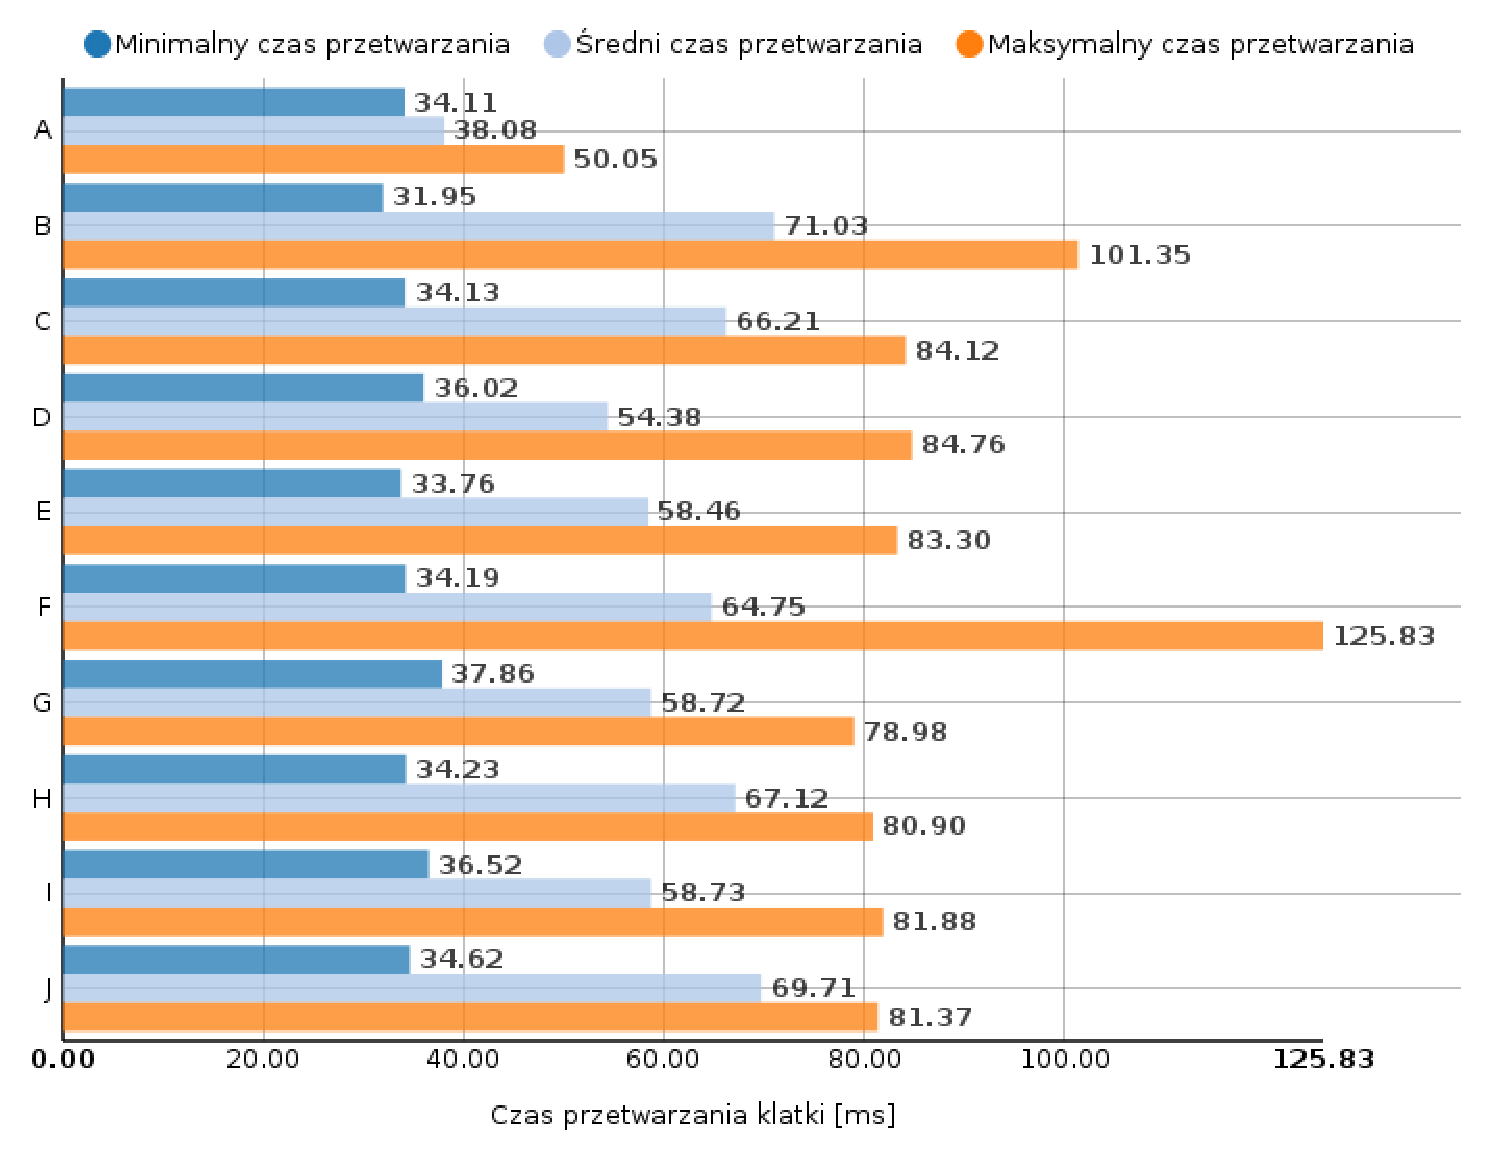
\includegraphics[width=12cm]{charts/timing/RandomForGestureC}
        \caption[Czas przetwarzania klatki każdej osoby dla gestu C (las drzew losowych)]
                {Czas przetwarzania klatki każdej osoby dla gestu\\\textit{Wielka Litera C} (las drzew losowych)}
        \label{fig:RandomForGestureC}
      \end{figure}

      \begin{figure}[!ht]
        \centering
        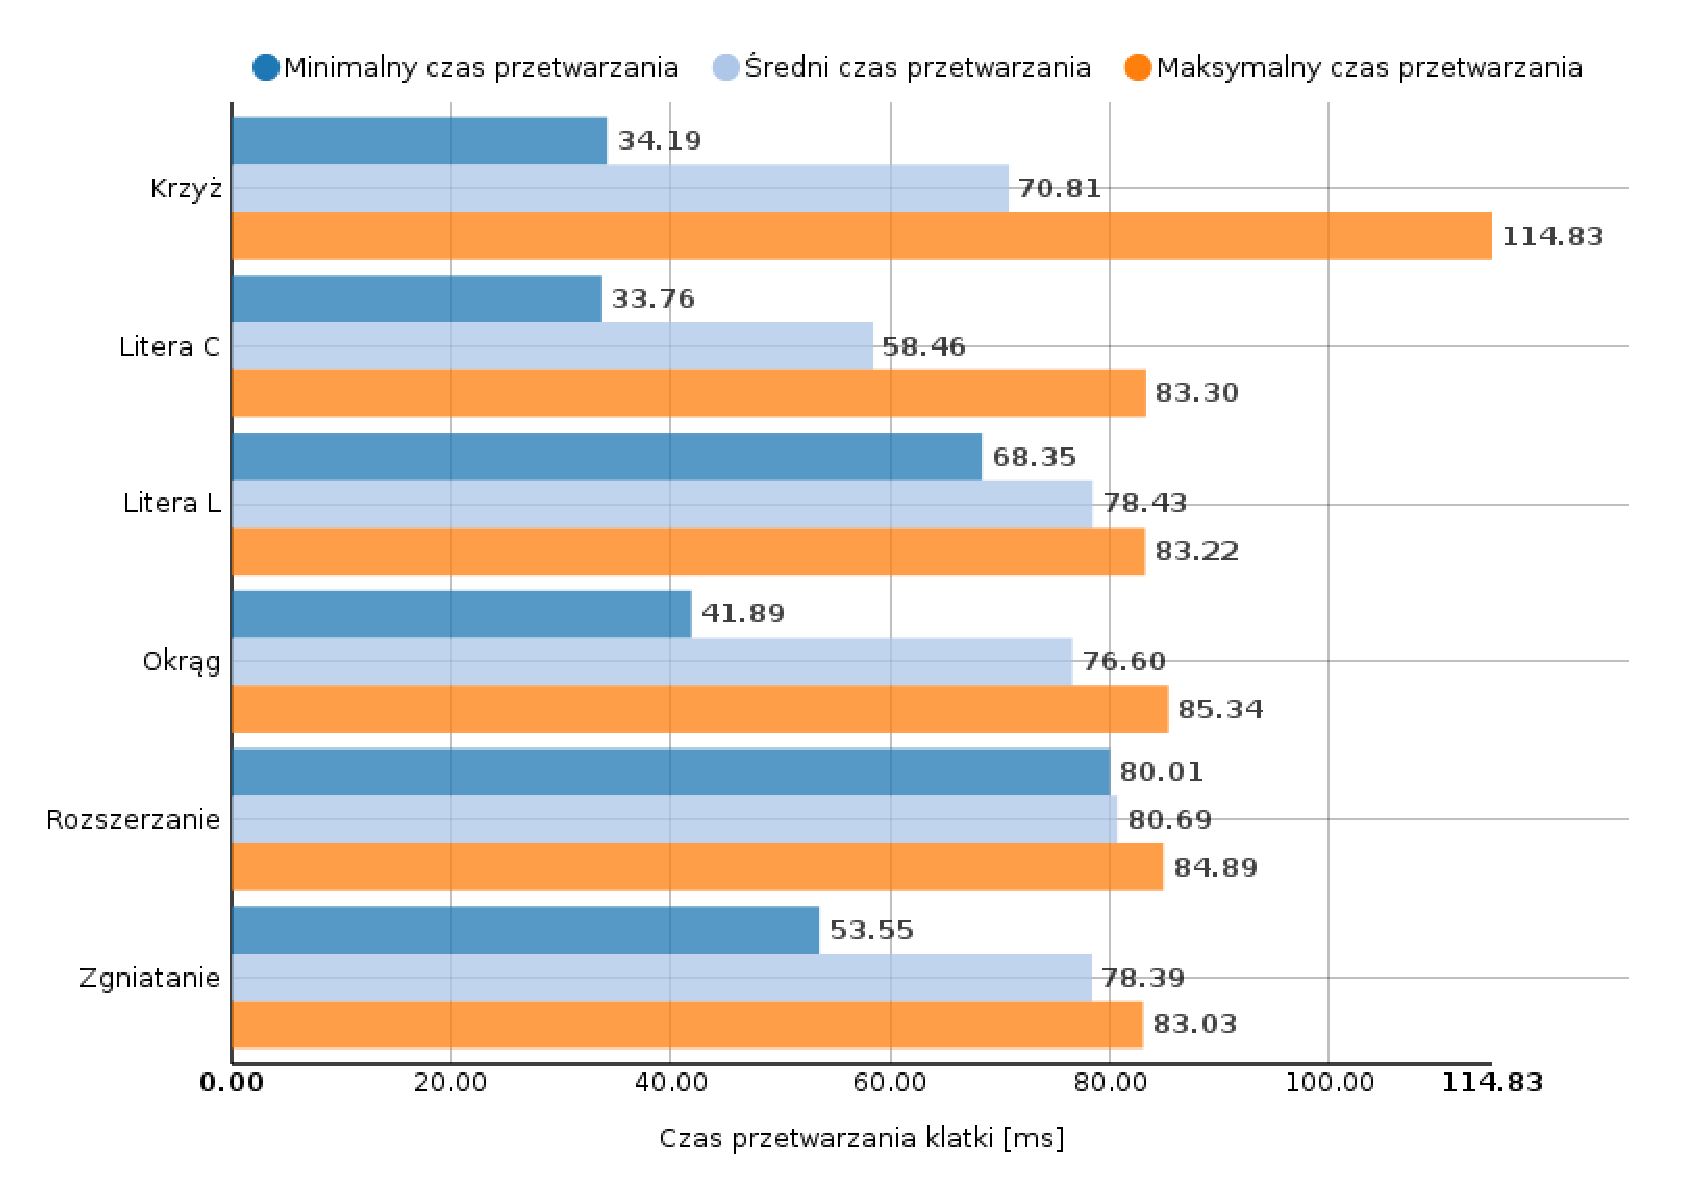
\includegraphics[width=12cm]{charts/timing/RandomTimingForPersonE}
        \caption[Czas przetwarzania klatki każdego gestu dla osoby E (las drzew losowych)]
                {Czas przetwarzania klatki każdego gestu dla osoby \textit{E}\\(las drzew losowych)}
        \label{fig:RandomTimingForPersonE}
      \end{figure}

    \newpage
    Jak widać na wykresie \ref{fig:LearningTime} wprowadzony przez ten konkretny algorytm narzut czasowy jest znaczny oraz jest wprost proporcjonalny do liczby wytrenowanych drzew. Jest to największa wada algorytmu jeśli chodzi o~wydajność. Każda metoda wykorzystująca uczenie maszynowe, wprowadza spory narzut przeznaczony na przygotowanie klasyfikatora. Nie jest to jednak argument dyskryminujący, ponieważ przygotowana implementacja pozwala na dalsze optymalizacje i~zminimalizowanie czasu uczenia (usprawnienia zostały zebrane w~sekcji \ref{Section_Usprawnienia}).

      \begin{figure}[!ht]
        \centering
        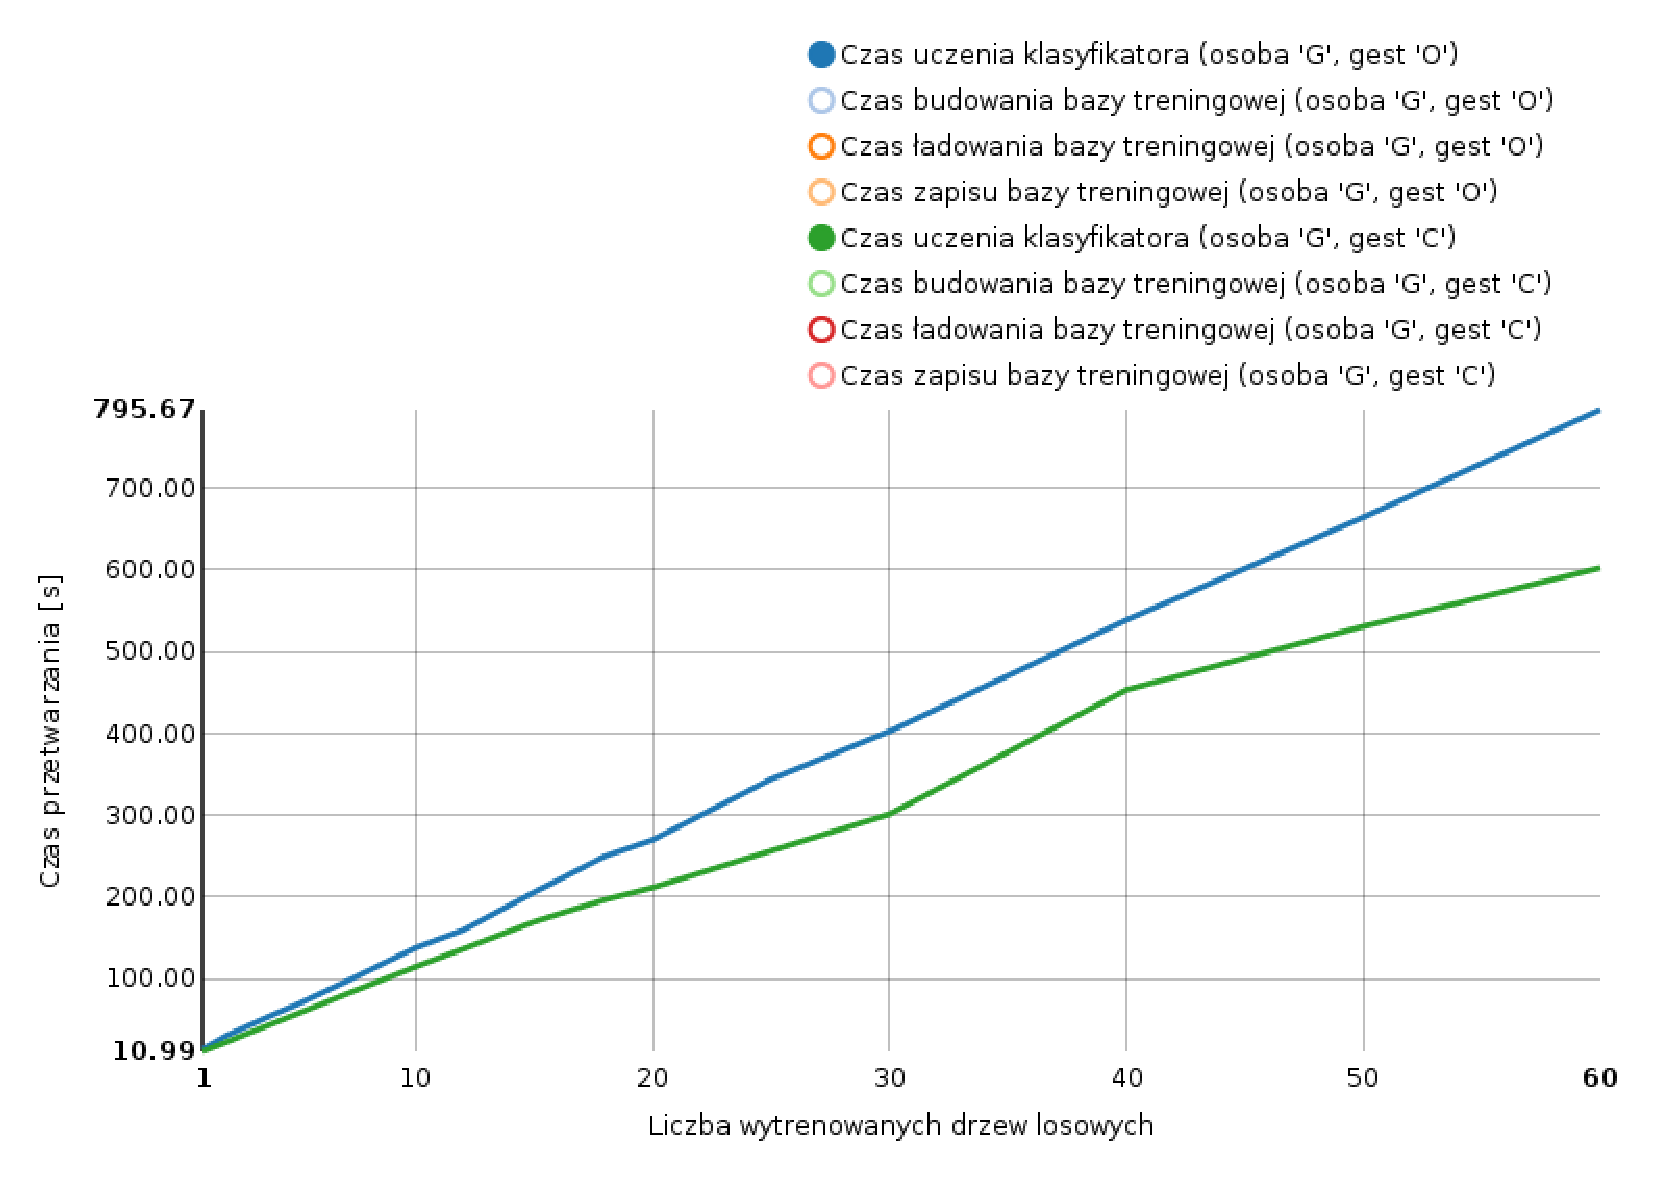
\includegraphics[width=13cm]{charts/timing/LearningTimePerTrainedTreesAmount}
        \caption[Czas nauki klasyfikatora w~zależności od liczby drzew losowych]
                {Czas nauki klasyfikatora w~zależności od liczby drzew losowych}
        \label{fig:LearningTime}
      \end{figure}

    Dla czasu przetwarzania klatki liczba drzew losowych ma niewielkie znaczenie. Wahania średniego czasu przetwarzania zaprezentowane na wykresie \ref{fig:TimingPerTrainedTreesAmount} mieszczą się w~przedziale o~szerokości około 20 milisekund. Dodatkowo widać, że im większa wytrenowanych drzew losowych tym stabilniejsza średnia wartość, jednocześnie nieznacznie zwiększa się minimalna wartość (wartości maksymalne czasu przetwarzania silnie zależą od określonej próbki).

      \begin{figure}[!ht]
        \centering
        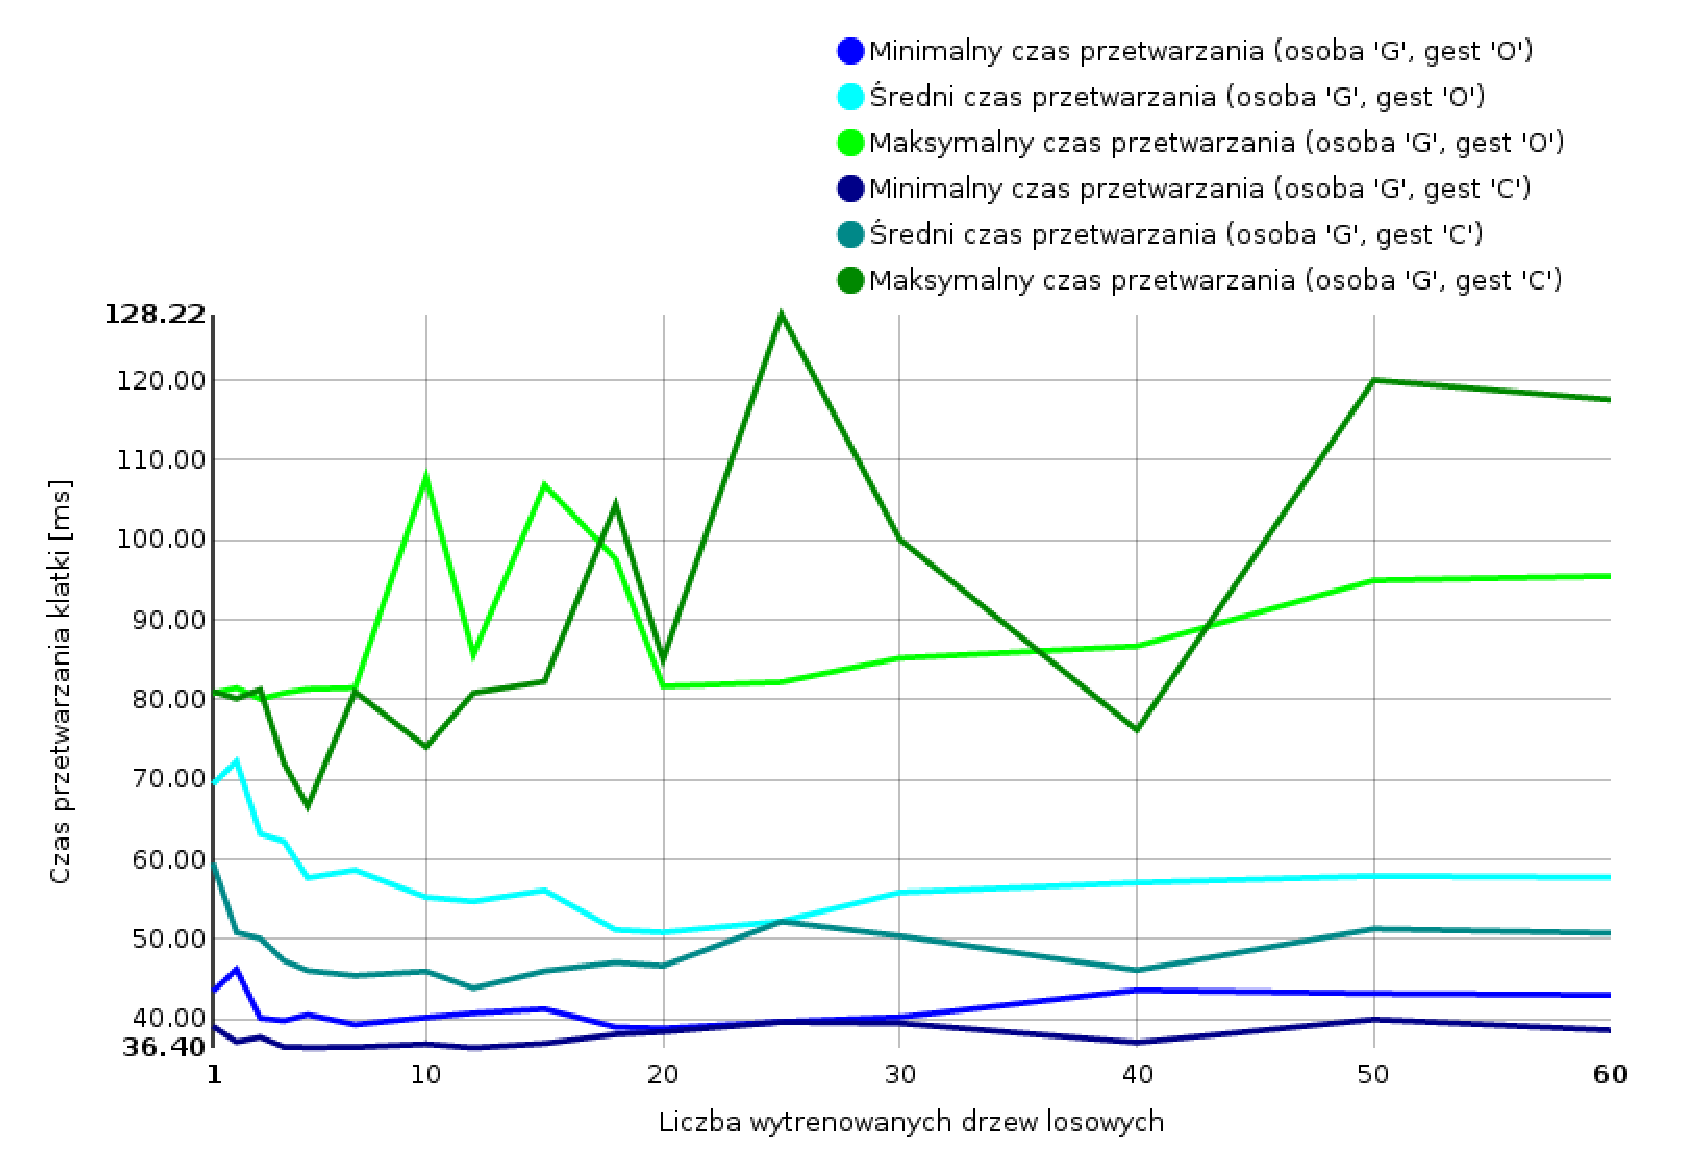
\includegraphics[width=13cm]{charts/timing/RandomTimingPersonG_OC_perTrainedTrees}
        \caption[Czas przetwarzania klatki w~zależności od liczby wytrenowanych drzew losowych]
                {Czas przetwarzania klatki w~zależności od liczby wytrenowanych drzew losowych (próbki \textit{Person\_G\_O} oraz \textit{Person\_G\_C})}
        \label{fig:TimingPerTrainedTreesAmount}
      \end{figure}

    \newpage
    Rzadki przepływ optyczny jest algorytmem o~najniższym średnim czasie przetwarzania klatki. Widać to na wykresach \ref{fig:SparseForGestureC} oraz \ref{fig:SparseTimingForPersonE}. Algorytm najlepiej poradził sobie praktycznie z~każdym zbiorem (wyjątkiem jest zbiór \textit{A}, jednak średnia wartość jest i~tak najniższa spośród trzech implementacji).

    Również, jeśli chodzi o~podział ze względu na gesty omawiana implementacja jest najwydajniejsza. W~obu przypadkach wartości średnie przetwarzania klatki animacji nie przekraczają 40 milisekund, maksymalne - tylko w~jednym przypadku przekraczają 50 milisekund. Implementacja może zostać wykorzystana w~warunkach o~dużych wymaganiach jeśli chodzi o~narzut przetwarzania pojedynczej ramki sekwencji wideo.

    Omawiana metoda charakteryzuje się liniową zależnością czasu obliczeń na pojedynczej klatce w~zależności od maksymalnej liczby punktów charakterystycznych (wykres \ref{fig:TimingPerFeaturesAmount}) oraz zależnością zbliżoną do logarytmicznej jeśli chodzi o~minimalną odległość pomiędzy punktami wyznaczonymi przez algorytm (wykres \ref{fig:TimingPerMinimalDistance}).

      \begin{figure}[!ht]
        \centering
        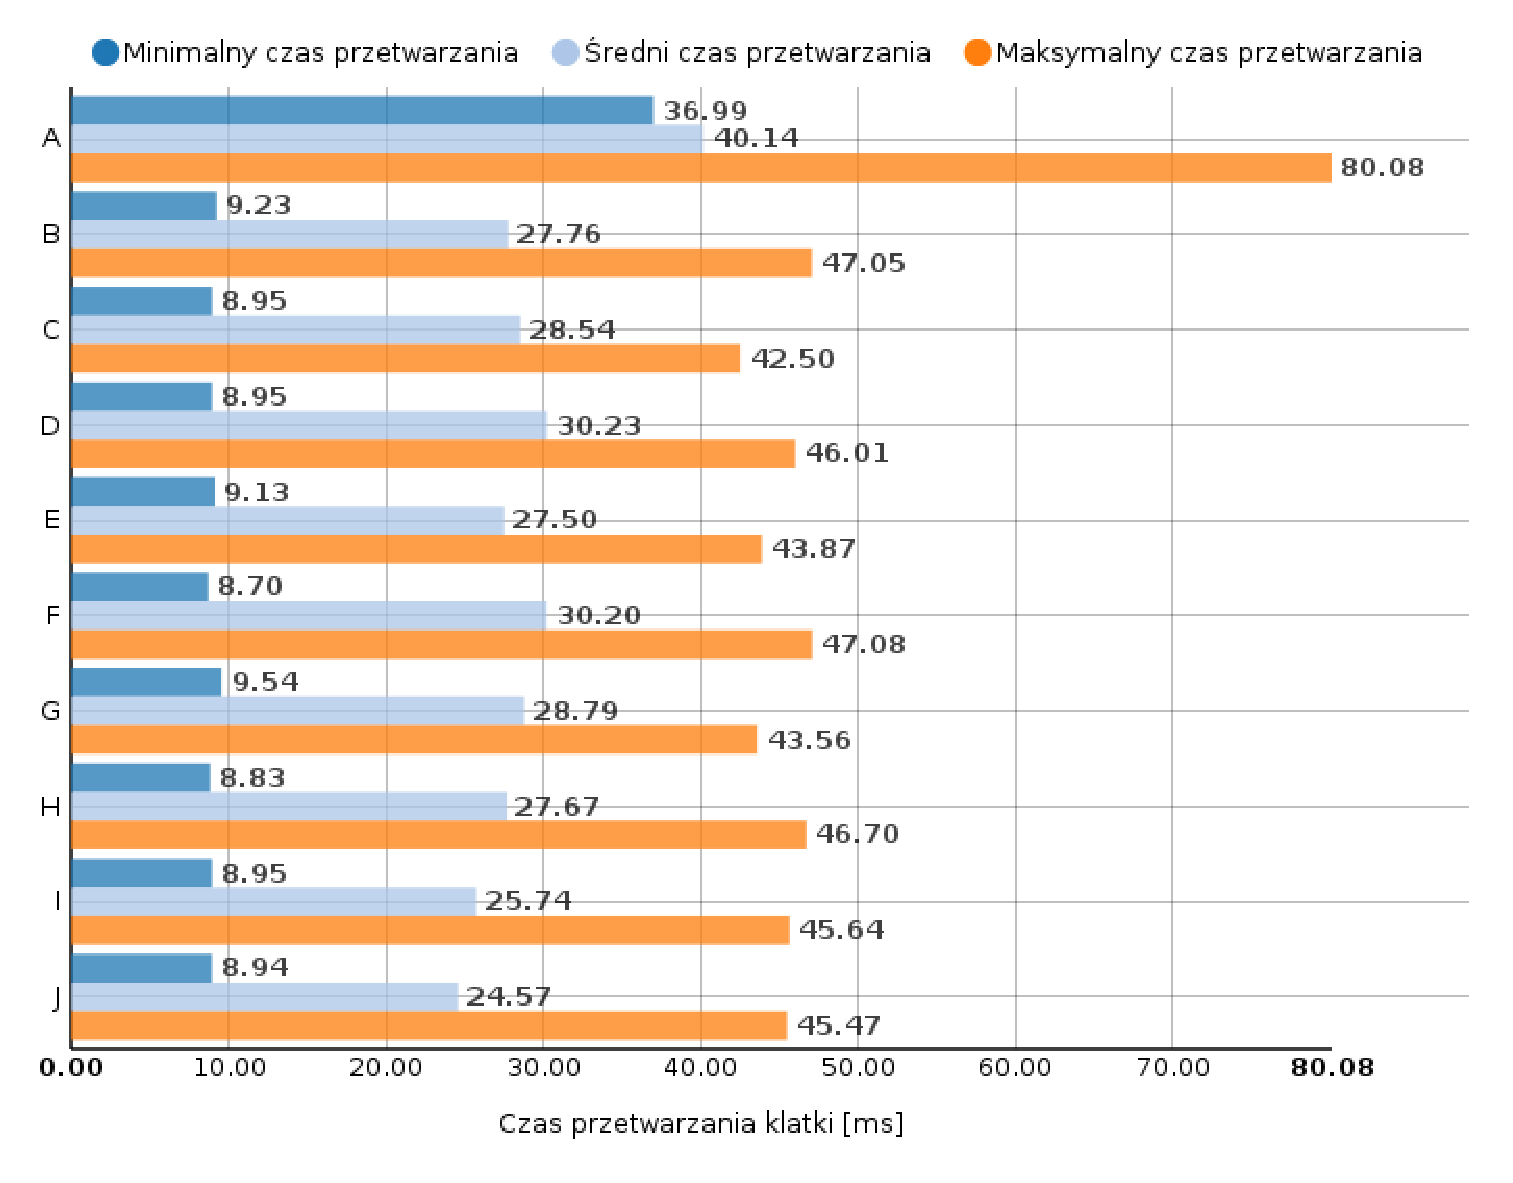
\includegraphics[width=12.5cm]{charts/timing/SparseForGestureC}
        \caption[Czas przetwarzania klatki każdej osoby dla gestu C (rzadki przepływ optyczny)]
                {Czas przetwarzania klatki każdej osoby dla gestu\\\textit{Wielka Litera C} (rzadki przepływ optyczny)}
        \label{fig:SparseForGestureC}
      \end{figure}

      \begin{figure}[!ht]
        \centering
        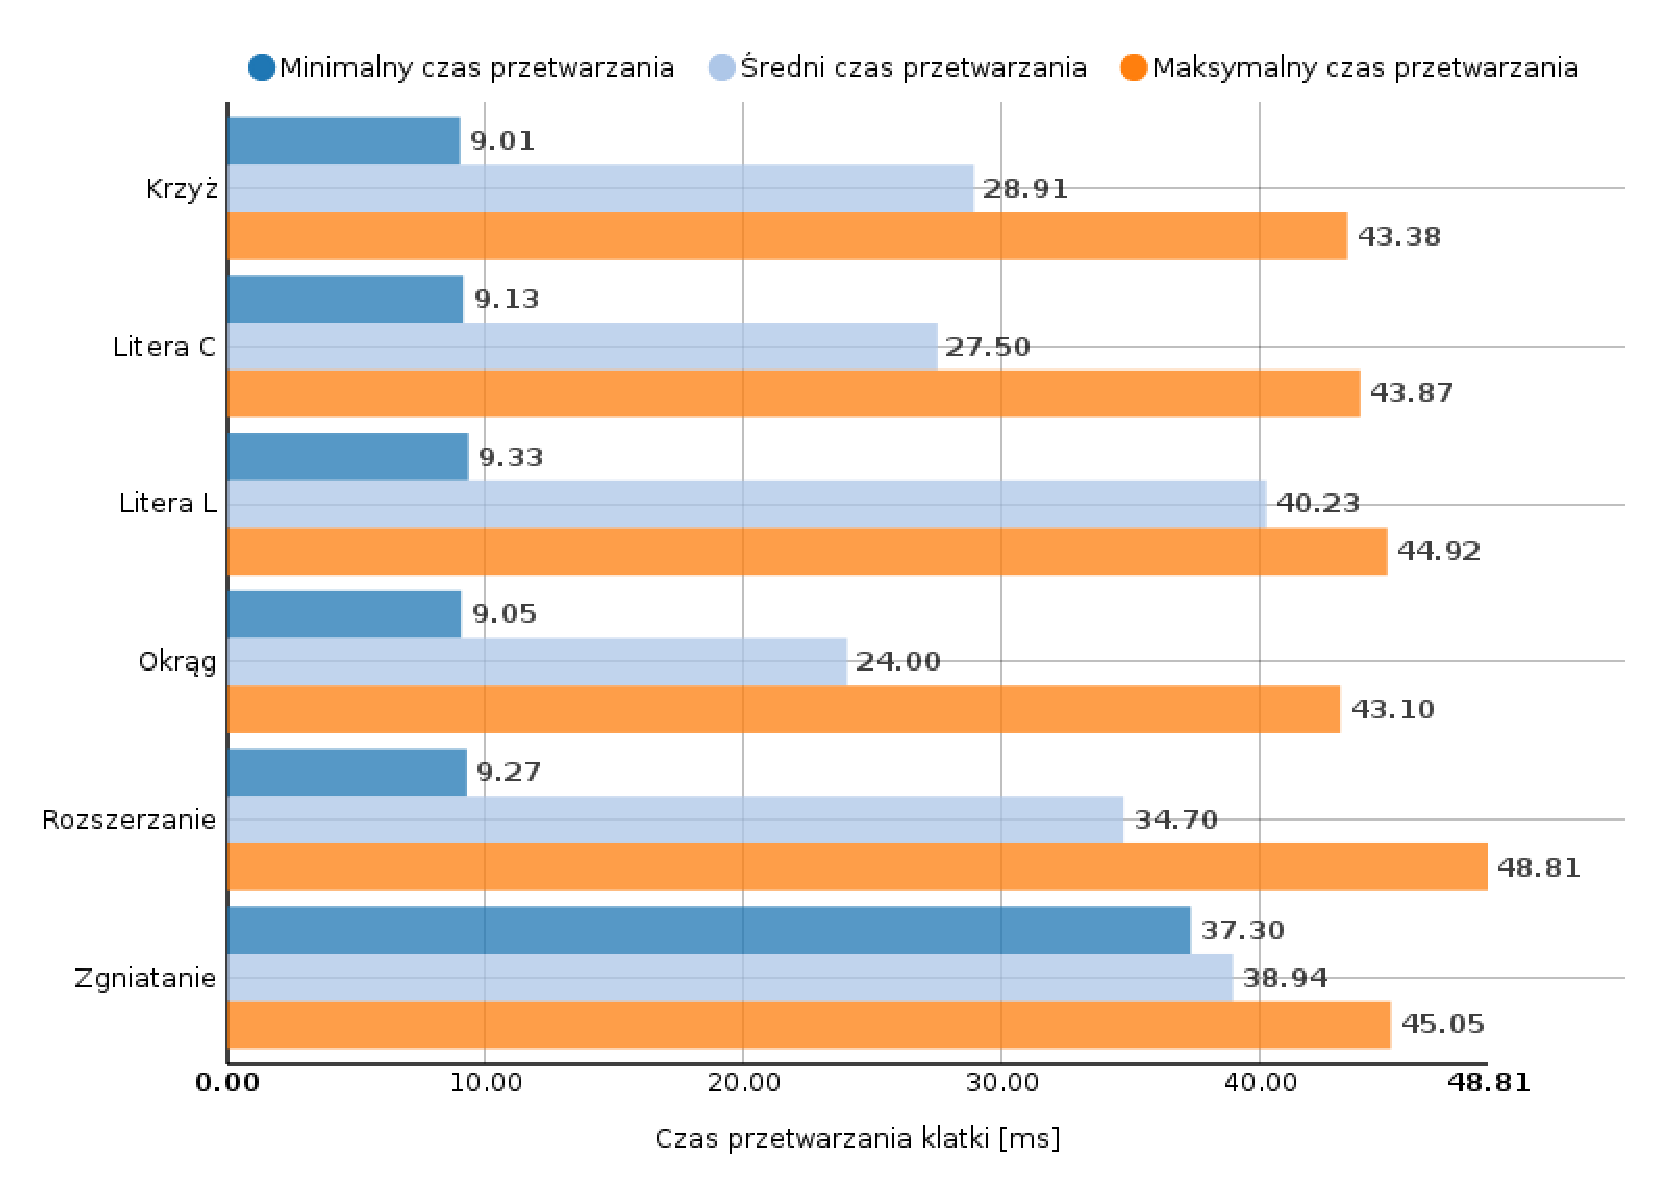
\includegraphics[width=12.5cm]{charts/timing/SparseTimingForPersonE}
        \caption[Czas przetwarzania klatki każdego gestu dla osoby E (rzadki przepływ optyczny)]
                {Czas przetwarzania klatki każdego gestu dla osoby \textit{E}\\(rzadki przepływ optyczny)}
        \label{fig:SparseTimingForPersonE}
      \end{figure}

    \newpage
      \begin{figure}[!ht]
        \centering
        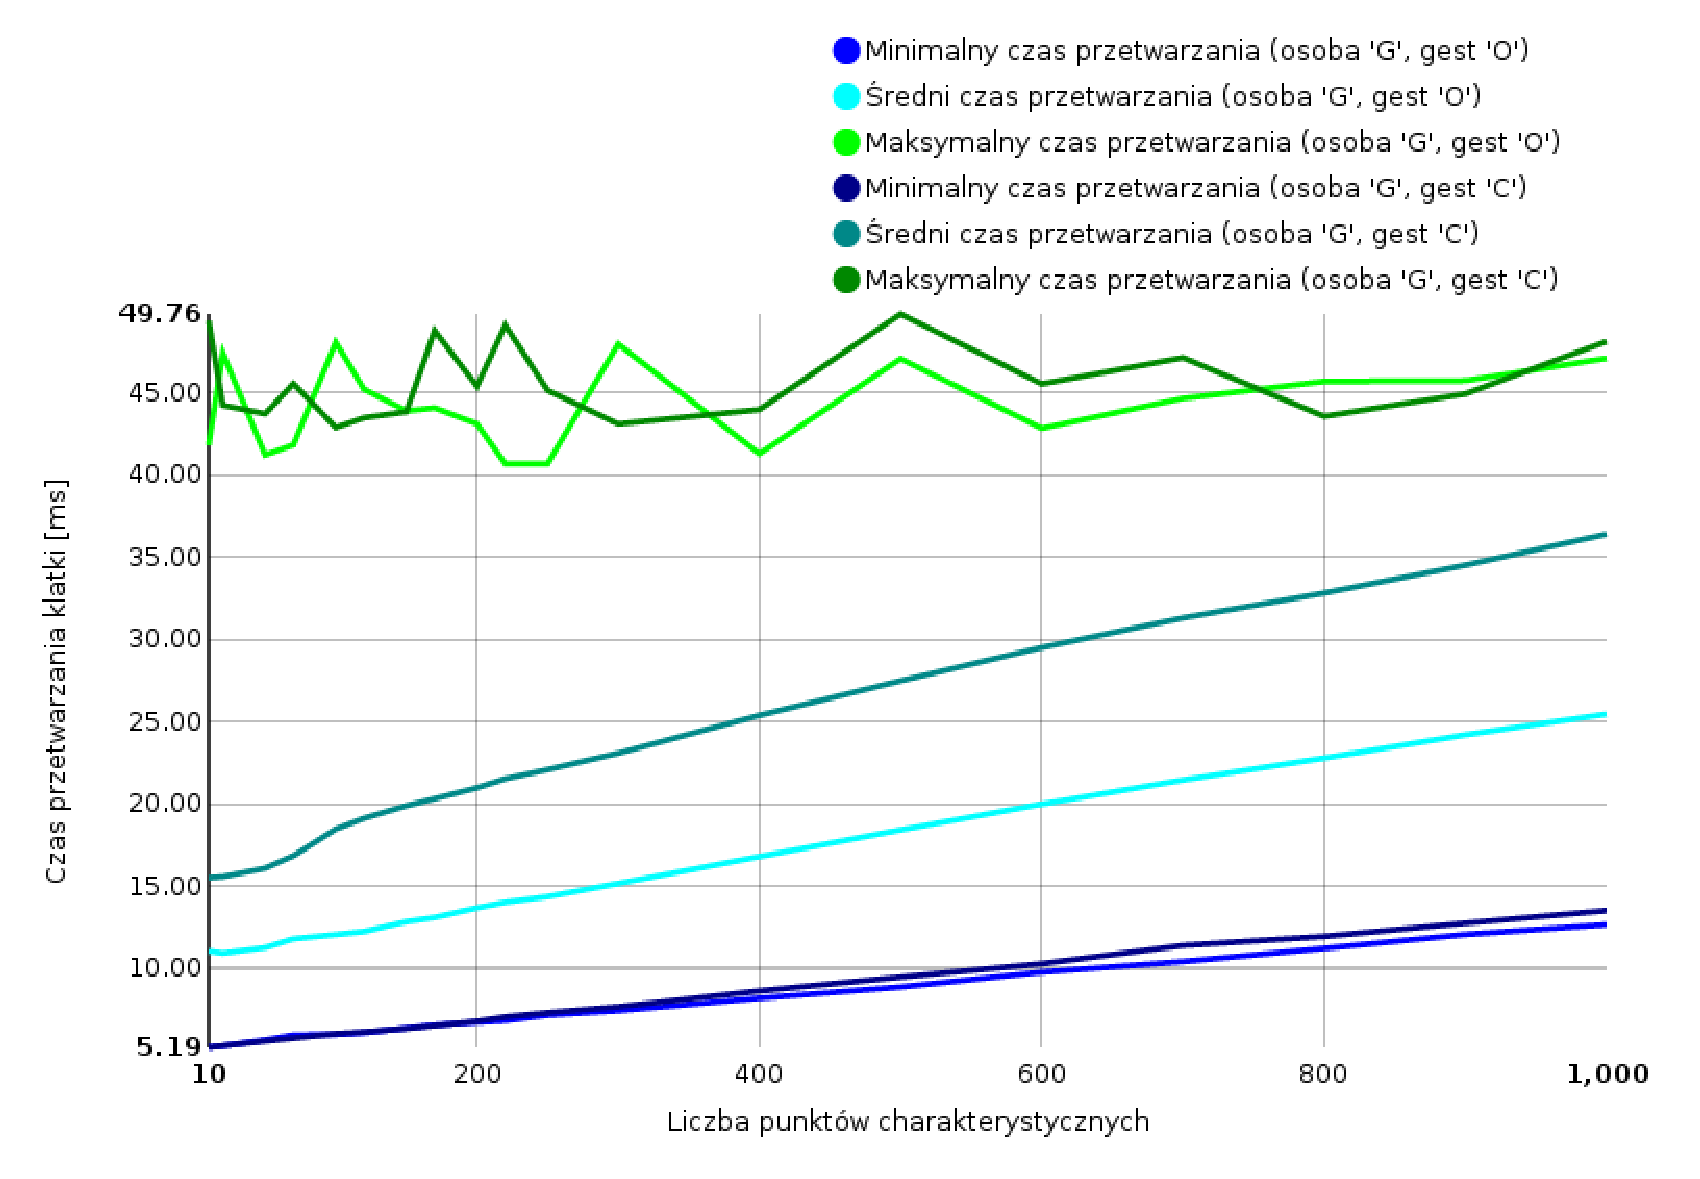
\includegraphics[width=12.5cm]{charts/timing/SparseTimingPersonG_OC_perFeaturesAmount}
        \caption[Czas przetwarzania klatki w~zależności od maksymalnej liczby punktów charakterystycznych]
                {Czas przetwarzania klatki w~zależności od maksymalnej liczby punktów charakterystycznych (próbki \textit{Person\_G\_O} oraz \textit{Person\_G\_C})}
        \label{fig:TimingPerFeaturesAmount}
      \end{figure}

      \begin{figure}[!ht]
        \centering
        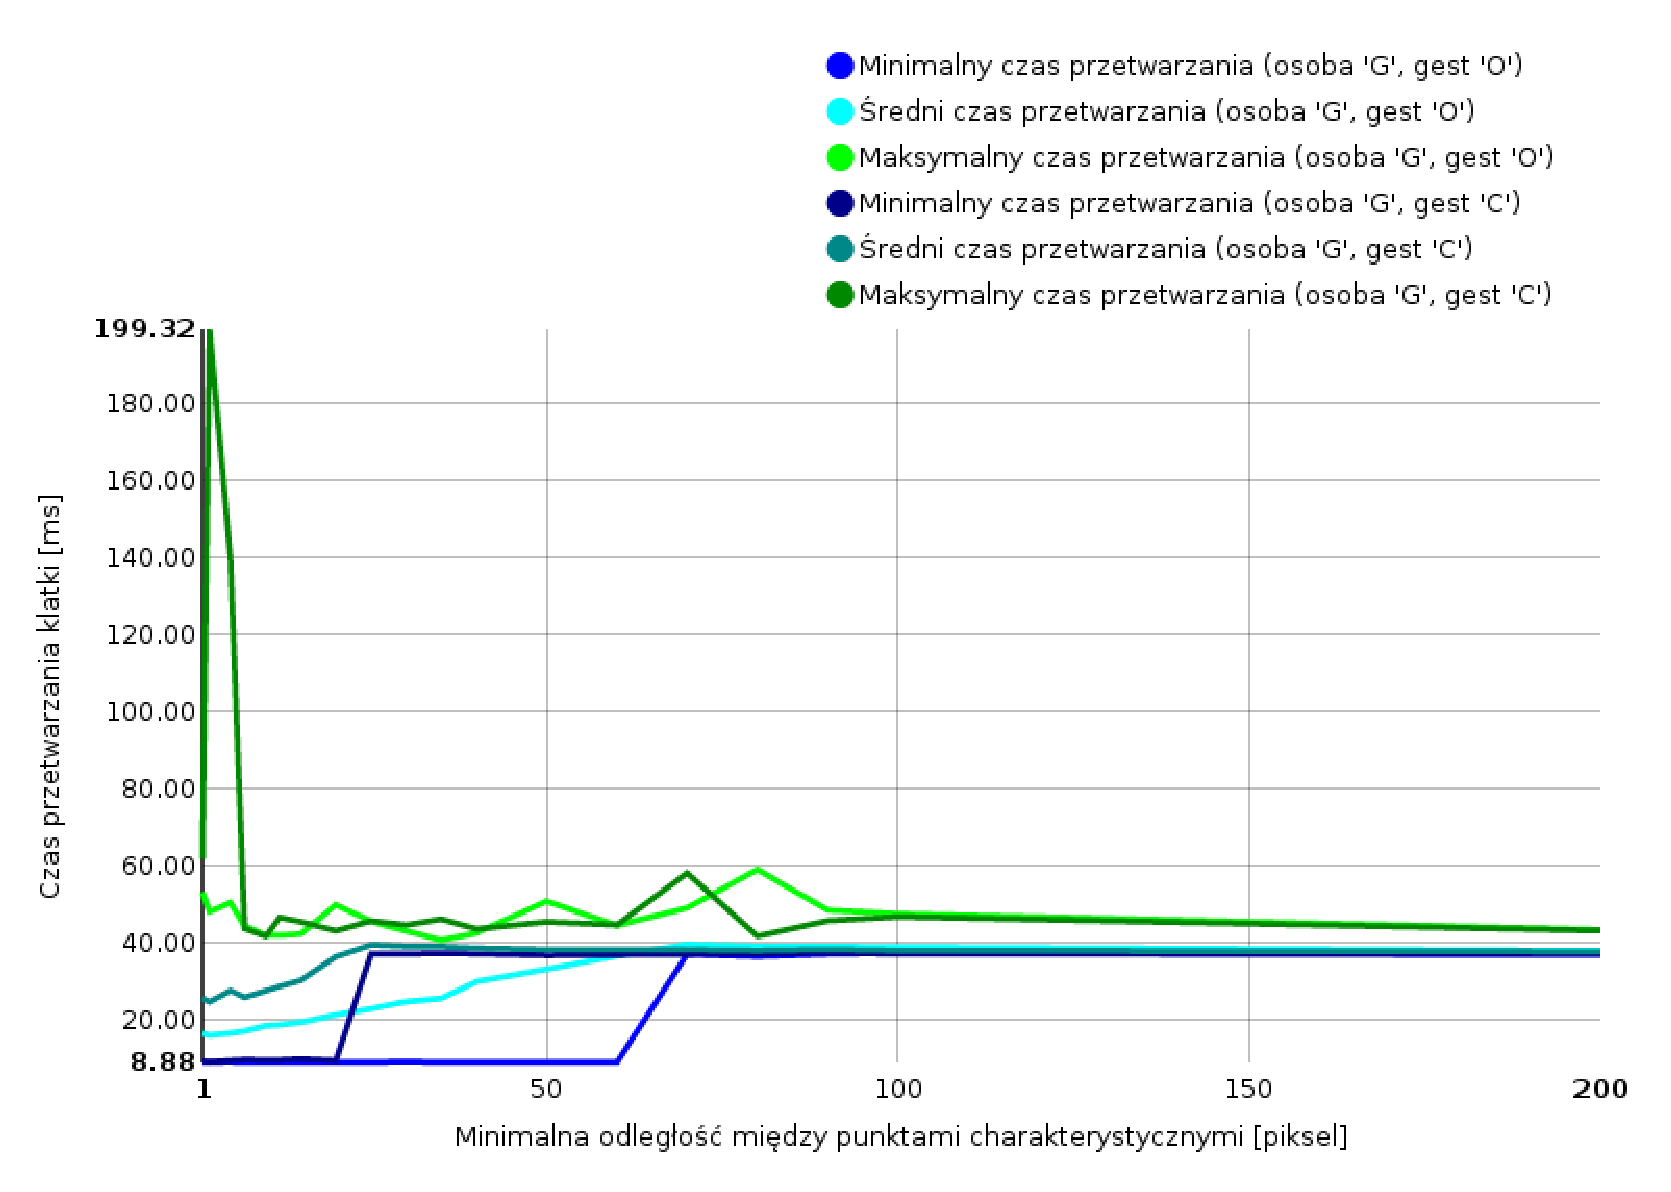
\includegraphics[width=12.5cm]{charts/timing/SparseTimingPersonG_OC_perMinimalDistance}
        \caption[Czas przetwarzania klatki w~zależności od minimalnej odległości pomiędzy punktami charakterystycznymi]
                {Czas przetwarzania klatki w~zależności od minimalnej odległości pomiędzy punktami charakterystycznymi (próbki \textit{Person\_G\_O} oraz \textit{Person\_G\_C})}
        \label{fig:TimingPerMinimalDistance}
      \end{figure}

  \section{Wprowadzony narzut czasowy}\label{Section_Overhead}
    Na podstawie wyników zaprezentowanych w~poprzedniej sekcji można skutecznie określić, który algorytm wprowadza najmniejszy całkowity narzut czasowy przetwarzania sekwencji wideo. Na wykresie \ref{fig:OverheadGL} zostały zestawione wartości dla każdego z~algorytmów. Najbardziej optymalnym algorytmem jest algorytm przepływu optycznego w~wariancie rzadkim.

    Porównanie zawarte na wykresie omówionym powyżej, nie zawiera pełnego narzutu dla metody opartej o~uczenie maszynowe. Całkowite podsumowanie zostało umieszczone na rysunku \ref{fig:RandomForestTrackerOverhead}. Widać wyraźnie, że w~przypadku pełnej generacji (zapisu, odczytu i~budowania bazy treningowej) dla jednego drzewa narzut jest ogromny (około 1 minuty). Mimo, iż narzut czasowy wprowadzony tylko poprzez klasyfikacji w~oparciu o~wytrenowany zbiór jest niski, to metoda jest bardzo kosztowna. W~sekcji \ref{Section_Usprawnienia} zwrócono uwagę na analizowany problem i~zaproponowano potencjalne rozwiązanie.

    Na wykresach \ref{fig:SpecialisedDenseOverhead}, \ref{fig:SpecialisedRandomOverhead} oraz \ref{fig:SpecialisedSparseOverhead} zaprezentowane zostały zależności całkowitego narzutu czasowego w~odniesieniu do podstawowych parametrów zaimplementowanych metod.

    W~przypadku algorytmu gęstego przepływu optycznego, narzut zmniejsza się wraz z~rozrzedzeniem siatki (zwiększeniem rozmiaru jej oczka) i~stabilizuje się w~okolicy rozmiaru równego 10 pikseli. Jak zostanie przedstawione w~następnym rozdziale wspomniana wartość może zostać przyjęta jako rozsądny kompromis pomiędzy jakością jak i~czasem działania algorytmu.

    Dla algorytmu wykorzystującego las drzew losowych całkowity narzut stabilizuje się wraz z~wykorzystaniem większej liczby drzew losowych. Biorąc pod uwagę czas wykonania, liczba pięciu drzew wydaje się rozsądnym kompromisem pomiędzy całkowitym narzutem czasowym oraz jakością.

    Dla algorytmu przepływu optycznego w~wariancie rzadkim mniejsze wartości minimalnej odległości pomiędzy punktami charakterystycznymi skutkują brakiem narzutu czasowego (wartość ujemna oznacza rezerwę jeśli chodzi o~czas przetwarzania). Biorąc jednak pod uwagę jakość omówioną w~sekcji \ref{Section_Quality} warto zwiększyć ten współczynnik w~celu zwiększenia jakości wyznaczonej ścieżki.

    \newpage
      \begin{figure}[!ht]
        \centering
        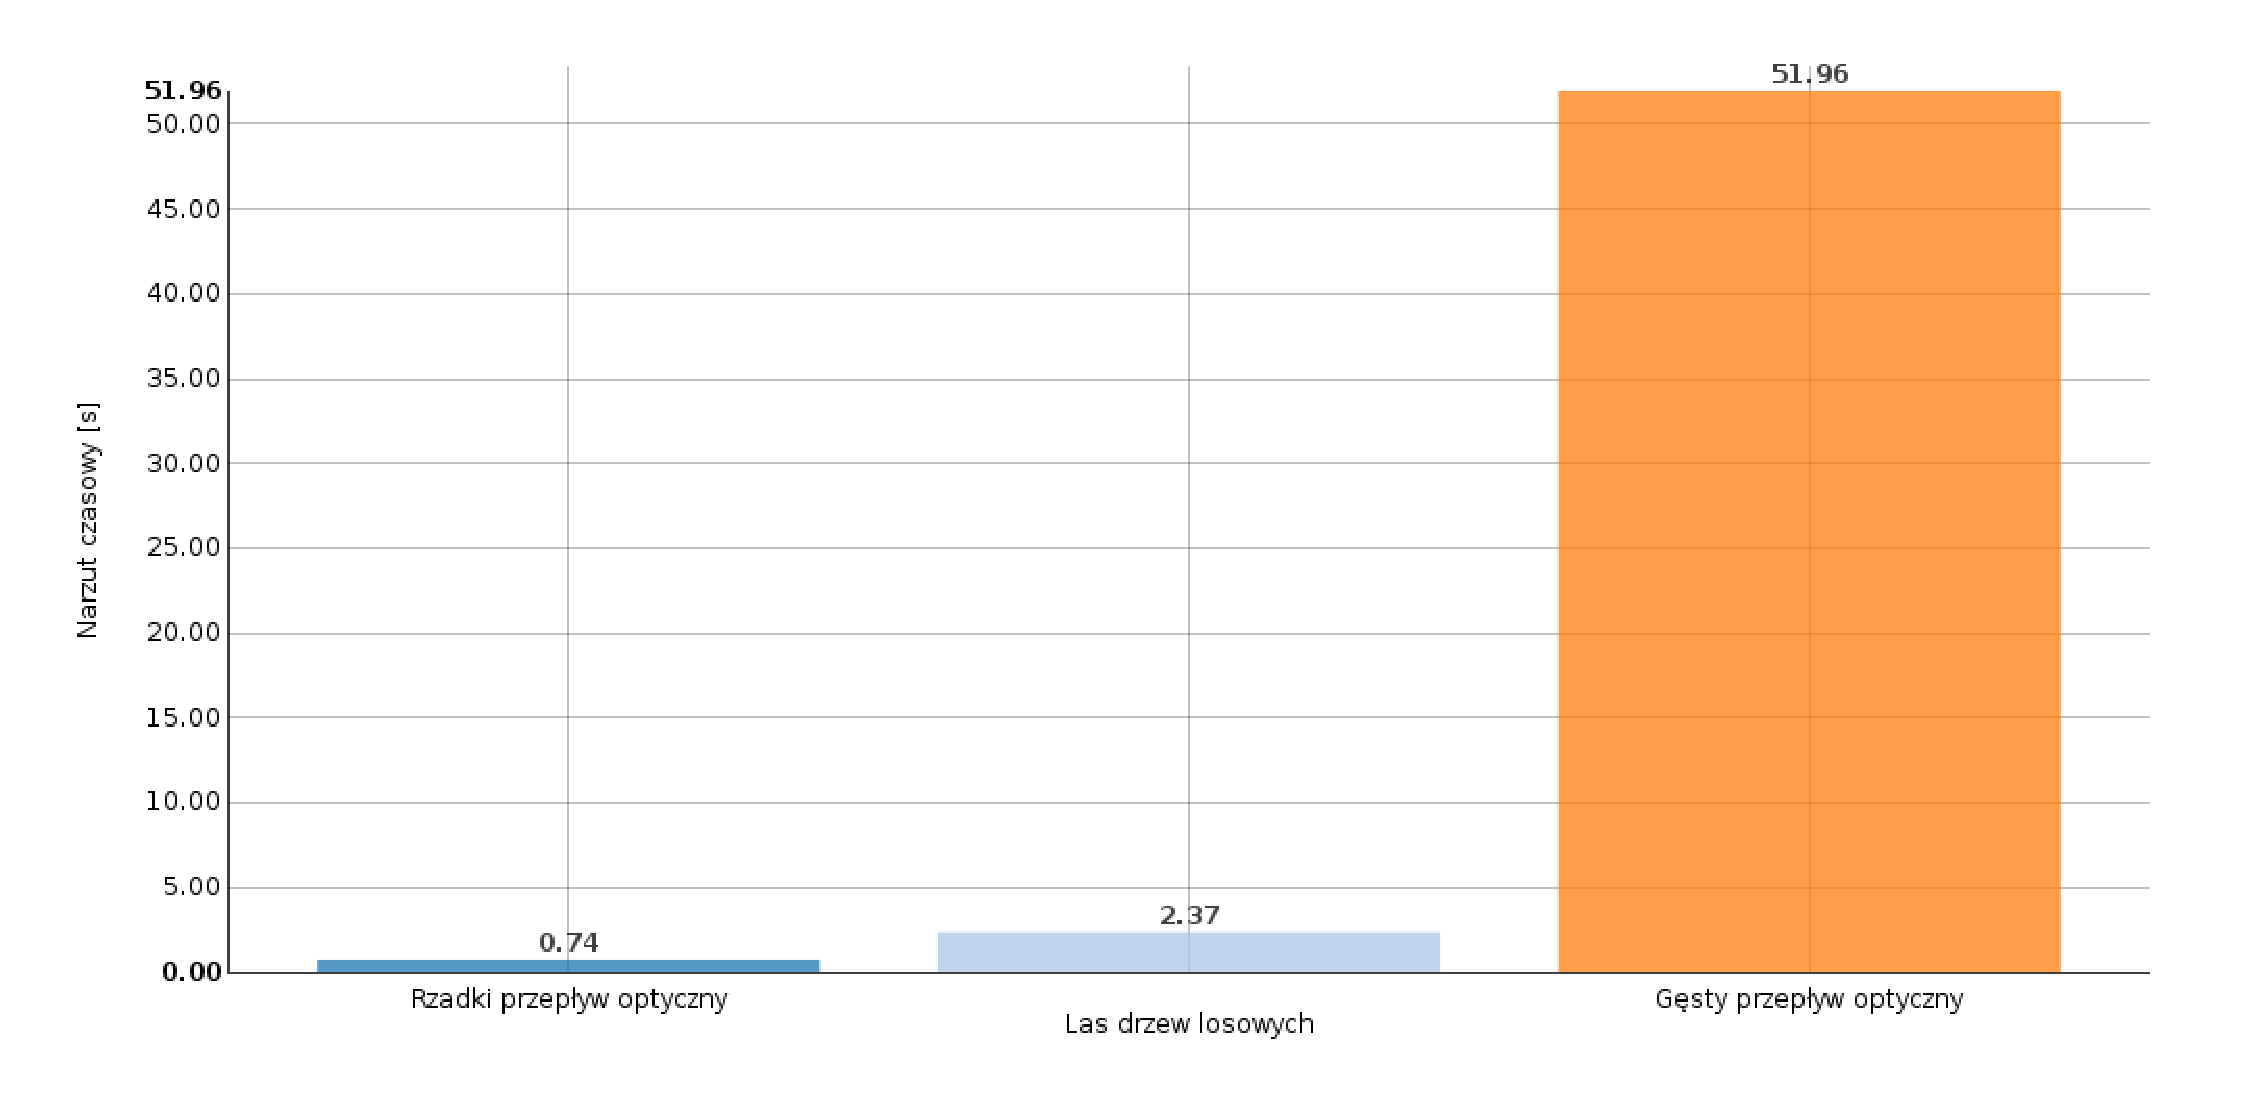
\includegraphics[width=14cm]{charts/overhead/OverheadGL}
        \caption[Narzut czasowy wprowadzony przez każdy algorytm]
                {Narzut czasowy wprowadzony przez każdy algorytm\\(próbka \textit{Person\_G\_L})}
        \label{fig:OverheadGL}
      \end{figure}

      \begin{figure}[!ht]
        \centering
        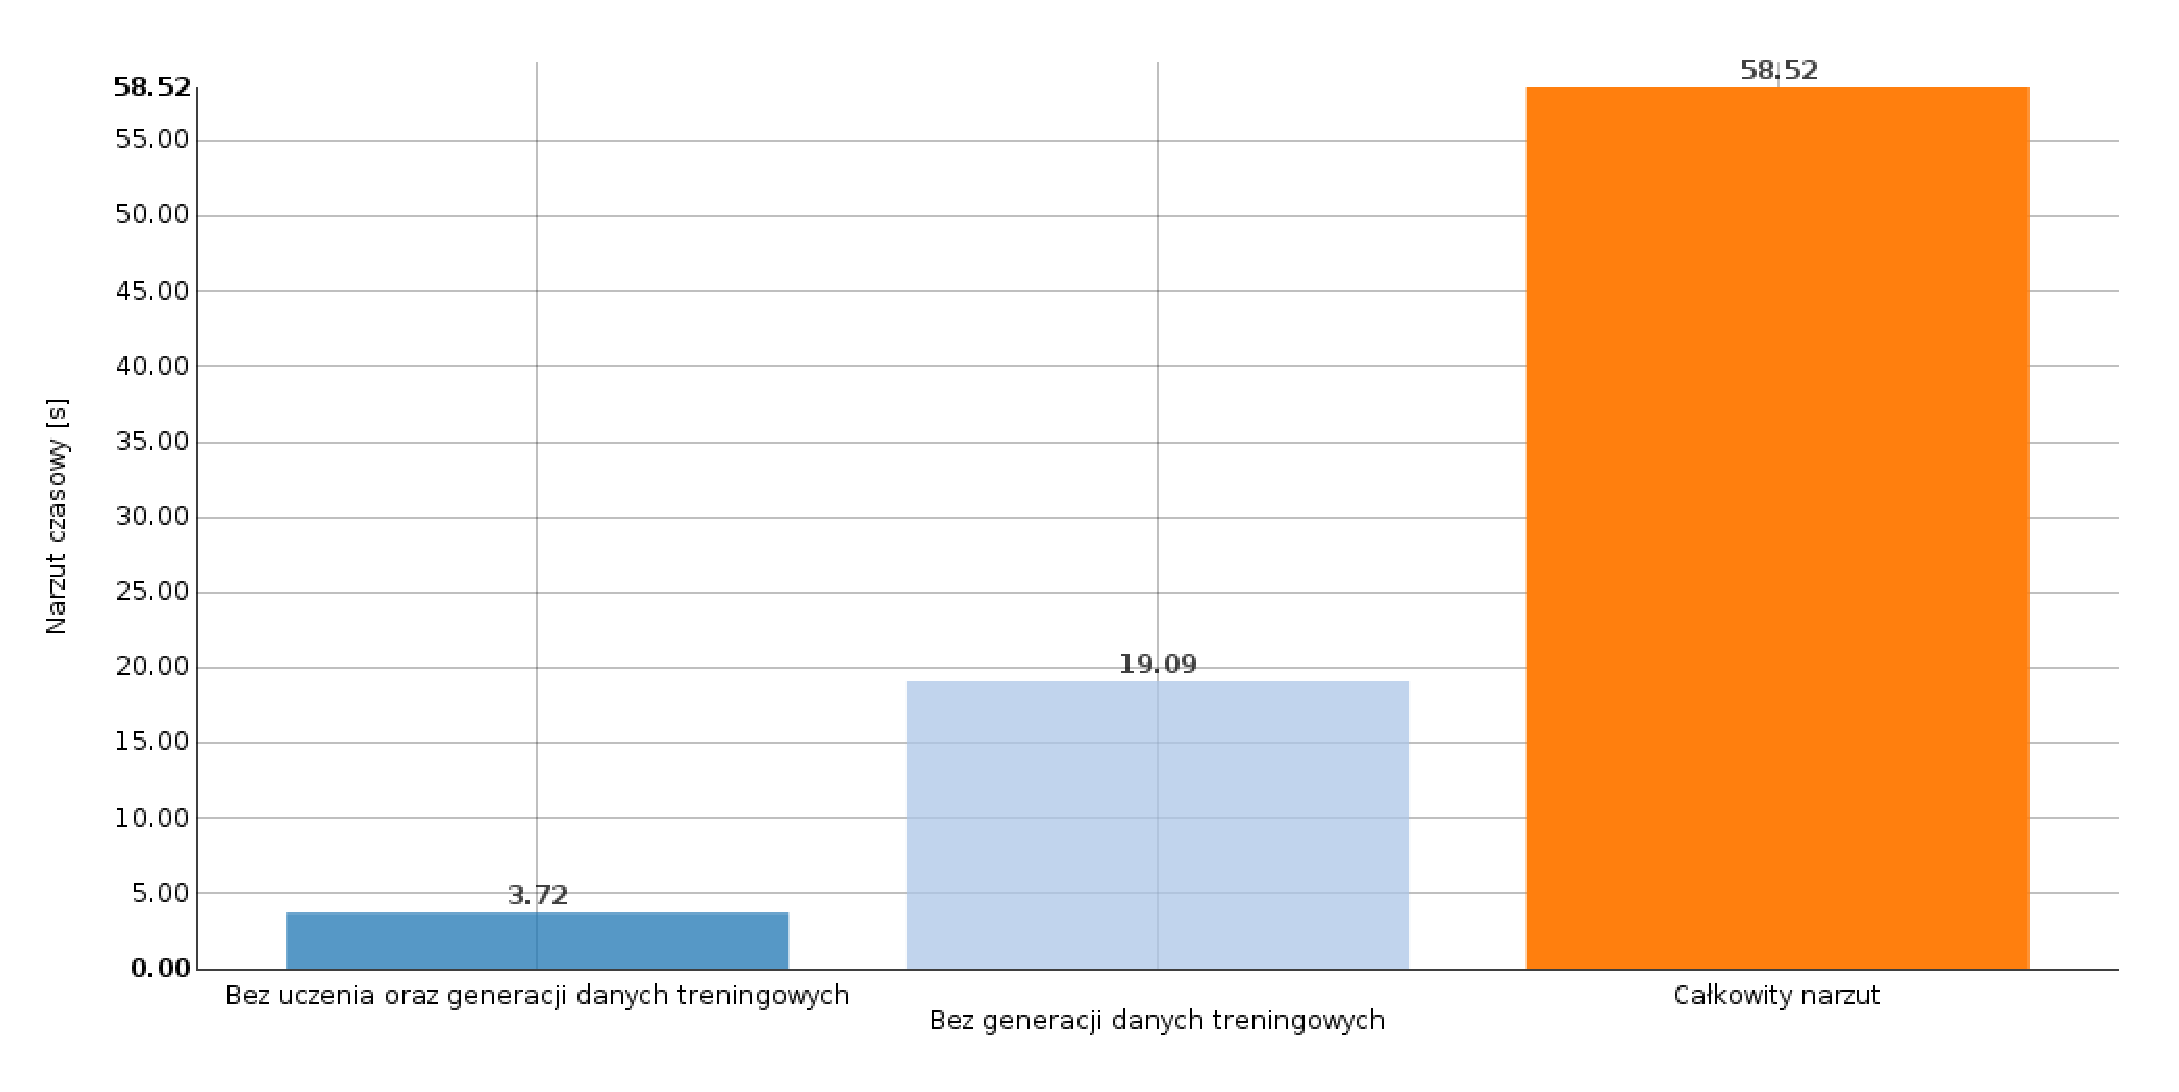
\includegraphics[width=14cm]{charts/overhead/RandomForestTrackerOverallOverhead}
        \caption[Całkowity narzut czasowy dla algorytmu wykorzystującego las drzew losowych]
                {Całkowity narzut czasowy dla algorytmu wykorzystującego las drzew losowych}
        \label{fig:RandomForestTrackerOverhead}
      \end{figure}

    \newpage
      \begin{figure}[!ht]
        \centering
        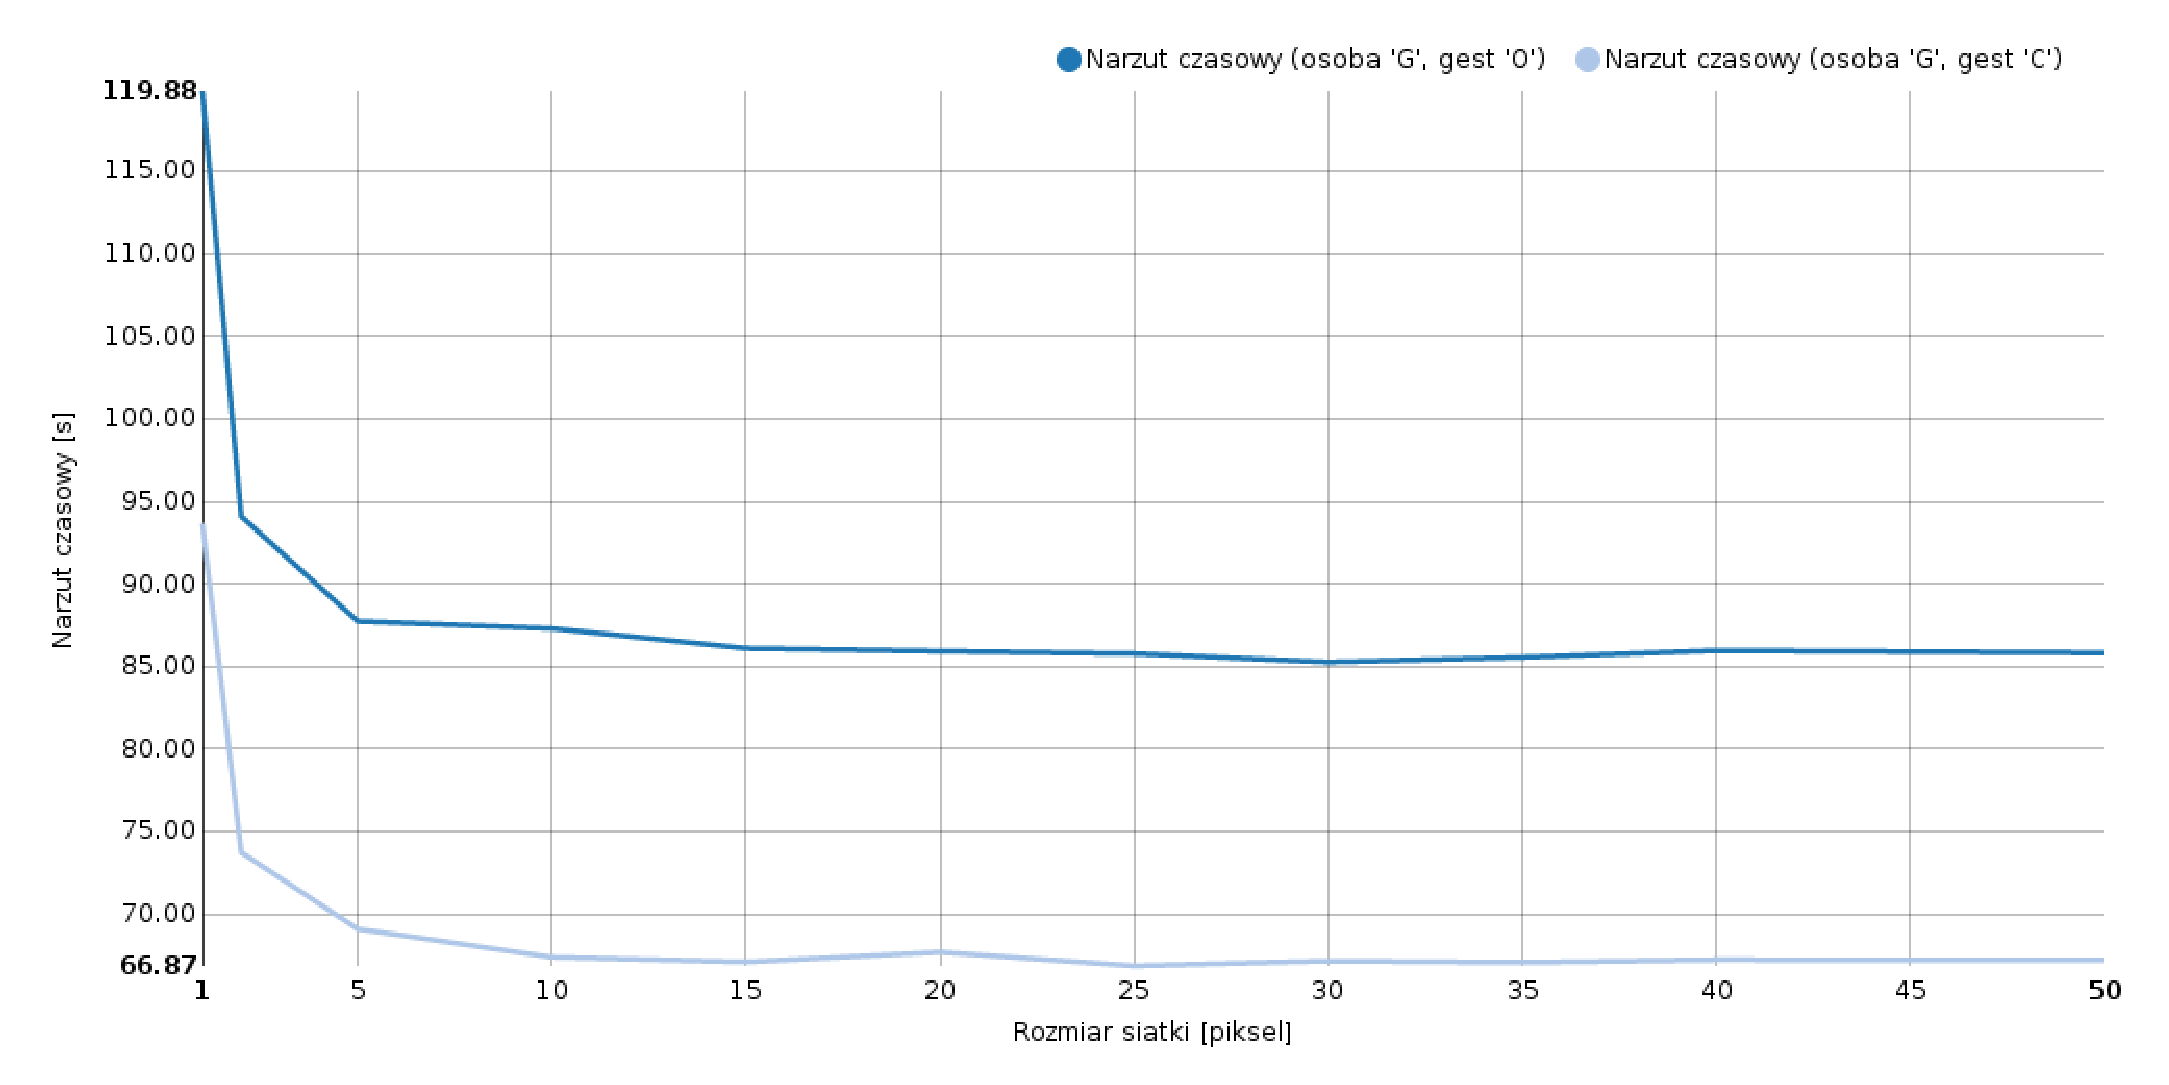
\includegraphics[width=10cm]{charts/overhead/DenseOverheadPerMapSize}
        \caption[Narzut czasowy w~zależności od rozmiaru siatki]
                {Narzut czasowy w~zależności od rozmiaru siatki\\(gęsty przepływ optyczny)}
        \label{fig:SpecialisedDenseOverhead}
      \end{figure}

      \begin{figure}[!ht]
        \centering
        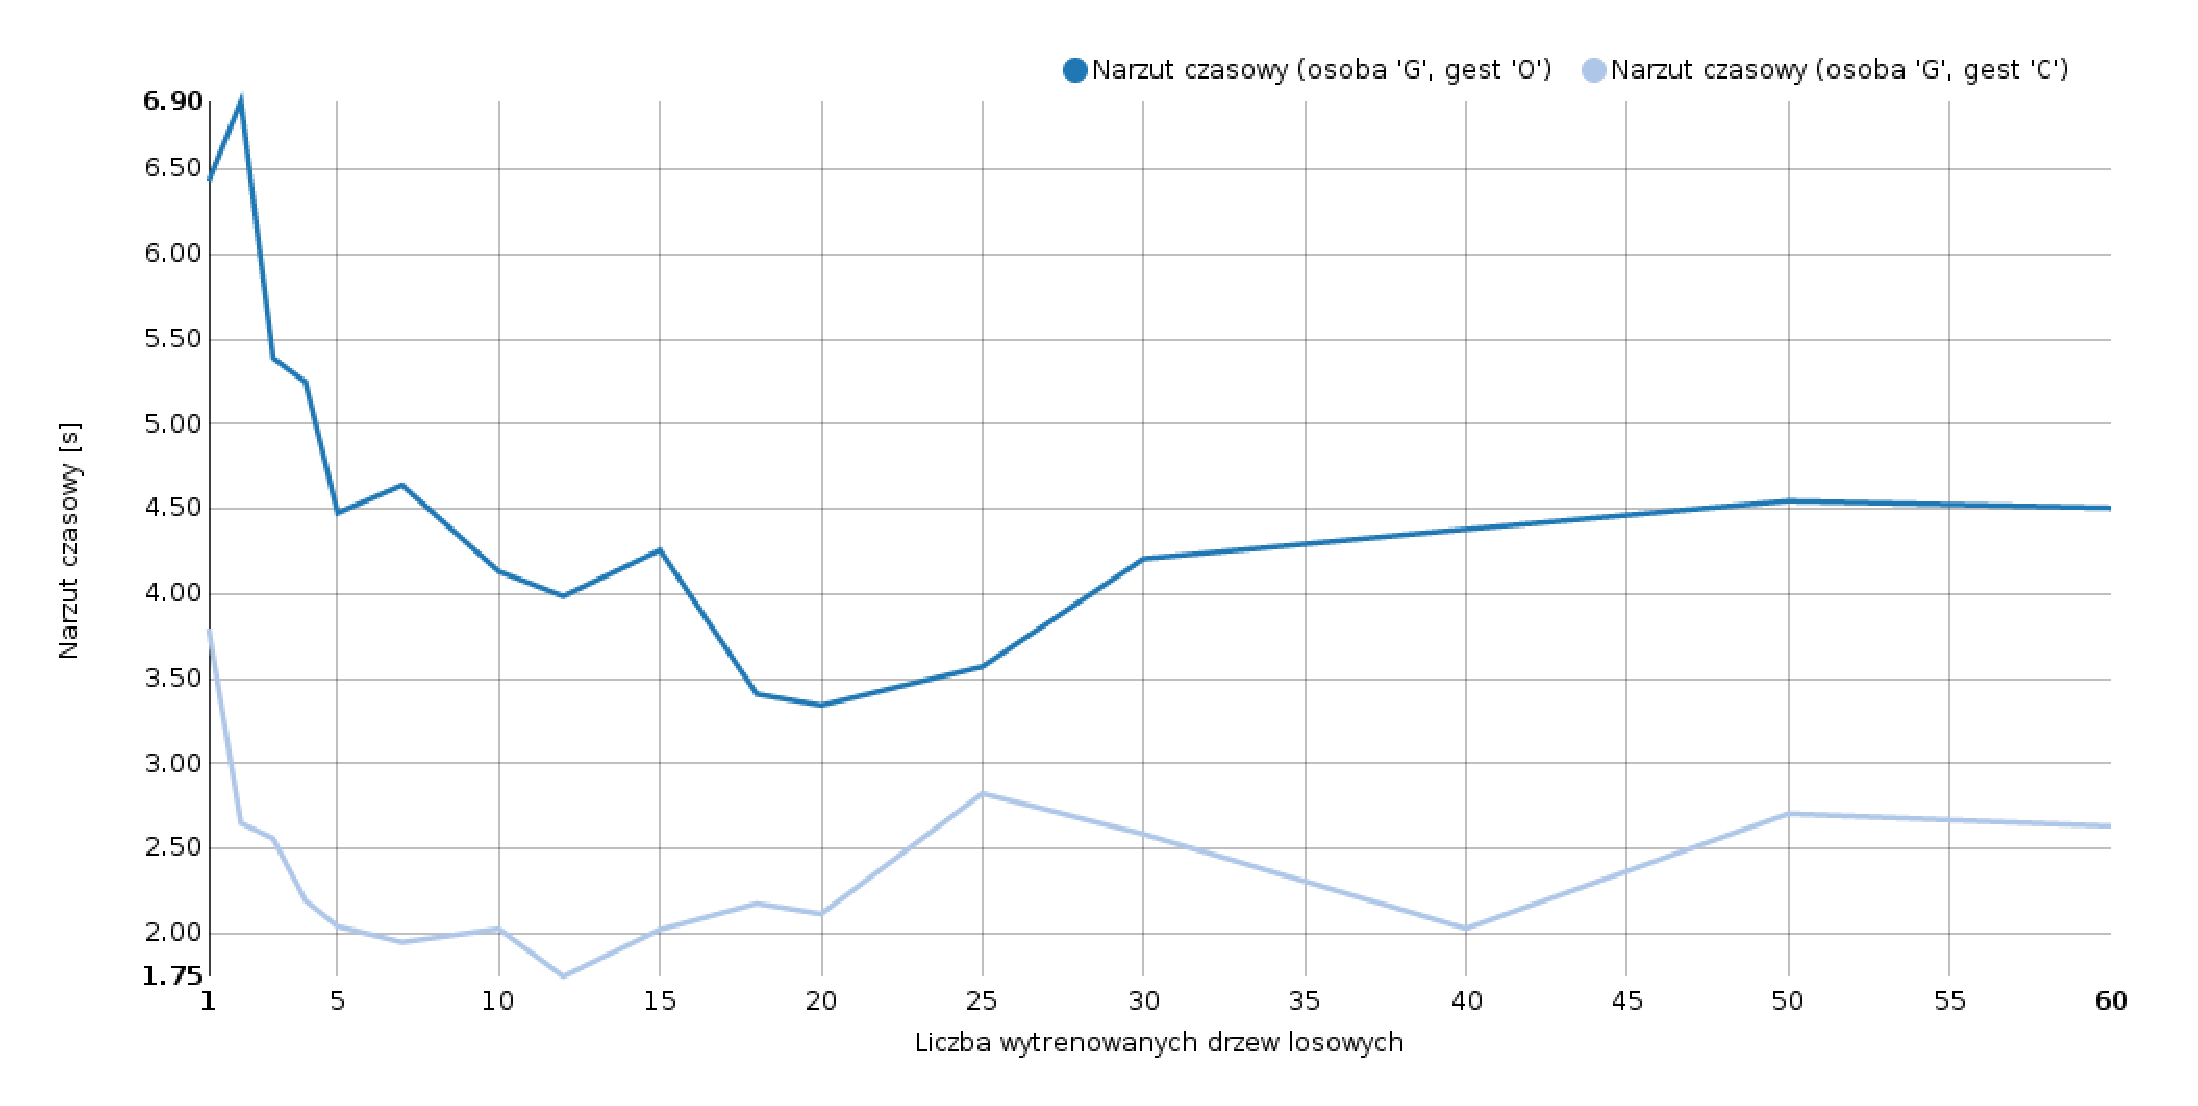
\includegraphics[width=10cm]{charts/overhead/RandomOverheadPerTrainedTreesAmount}
        \caption[Narzut czasowy w~zależności od liczby drzew losowych]
                {Narzut czasowy w~zależności od liczby drzew losowych\\(las drzew losowych)}
        \label{fig:SpecialisedRandomOverhead}
      \end{figure}

      \begin{figure}[!ht]
        \centering
        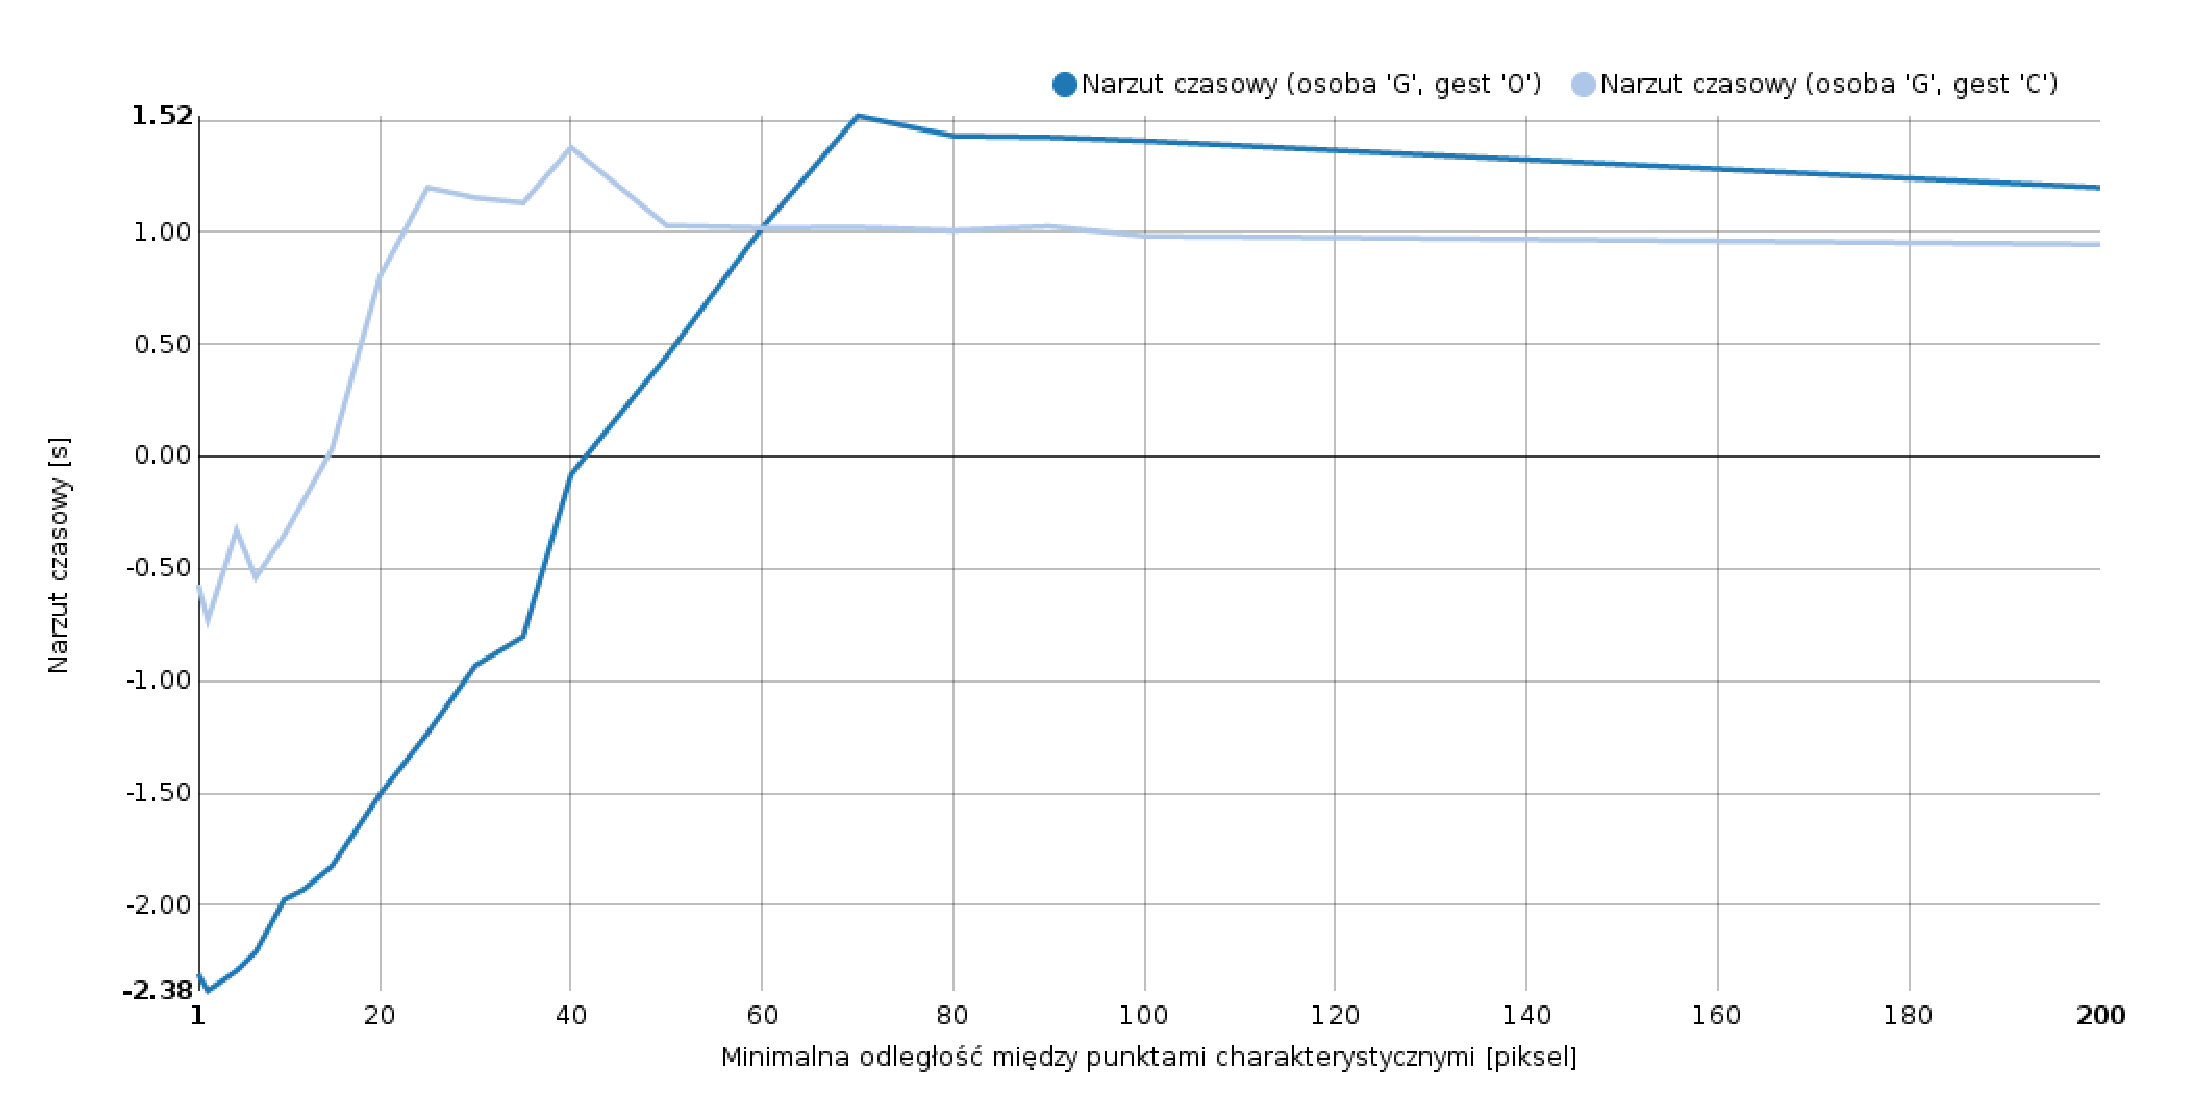
\includegraphics[width=10cm]{charts/overhead/SparseOverheadPerMinimalDistance}
        \caption[Narzut czasowy w~zależności od minimalnej odległości pomiędzy punktami charakterystycznymi]
                {Narzut czasowy w~zależności od minimalnej odległości pomiędzy punktami charakterystycznymi (rzadki przepływ optyczny)}
        \label{fig:SpecialisedSparseOverhead}
      \end{figure}

  \section{Weryfikacja jakości badanych algorytmów}\label{Section_Quality}

    Podstawowym elementem porównawczym jeśli chodzi o~jakość wyznaczonego rozwiązania, jest wartość odległości w~pikselach (w~metryce euklidesowej) od ścieżek i~punktów wzorcowych. Za pomocą wyznaczonych wartości jesteśmy w~stanie porównać jak bardzo zaproponowane przez algorytm rozwiązanie jest zbliżone do rozwiązania wyznaczonego manualnie dla każdej sekwencji wideo.

    Na serii wykresów od \ref{fig:DenseKeypointsPersonG} do \ref{fig:SparsePathGestureC} zostały zamieszczone wyniki badań jakościowych. Widać, że pod względem jakościowym dla wybranego zbioru \textit{G} oraz gestu o~nazwie \textit{Wielka litera C} najbardziej uniwersalnie radzi sobie algorytm rzadkiego przepływu optycznego. W~niewielkiej ilości przypadków maksymalna wartość odległości dla obu analizowanych parametrów wykracza poza przyjęty promień otaczający punkt wzorcowy.

    Nieco gorzej (zwłaszcza jeśli chodzi o~wariancje wartości maksymalnych i~minimalnych) radzi sobie algorytm oparty o~uczenie maszynowe. Wykorzystanie lasu drzew losowych dla przypadków brzegowych (np. zmiana kształtu dłoni) powoduje uzyskanie dużej wartości odległości co oznacza, że punkt został pominięty. Jest to niepożądana sytuacja, potencjalne usprawnienie zostało opisane w~sekcji \ref{Section_Usprawnienia}.

    Problematyczna sekwencja i~błędna klasyfikacja została dokładnie odzwierciedlona na wykresach \ref{fig:KeypointsQualityAC} oraz \ref{fig:KeypointsQualityGO}. Widać wyraźnie, że metoda oparta o~klasyfikator w~środkowej części wprowadza bardzo duży błąd rzutujący całościowo na jakość rozwiązania końcowego. Na wspomnianych wykresach widać również wyraźnie przewagę algorytmu przepływu optycznego w~wariancie rzadkim, jeśli chodzi o~odległość od punktów wzorcowych. W~przypadku odległości od ścieżek wzorcowych zdecydowanie najmniejszym błędem obarczona jest metoda wykorzystująca las drzew losowych, jednak jej nieprzewidywalność oraz duża wariancja mogą być wadą w~przypadku wdrożenia w~środowisku o~dużych wymaganiach dotyczących stabilności i~jakości.

    Algorytm przepływu optycznego w~wariancie gęstym radzi sobie lepiej dla sekwencji obarczonych dużym błędem w~poprzednio omawianej metodzie, jednak radzi sobie gorzej dla sekwencji poprawnie sklasyfikowanych przez algorytm wykorzystujący las drzew losowych. Jest to metoda pośrednia, o stabilnej i~przewidywalnej dokładności (co w~jej przypadku jest niewątpliwą zaletą, zwłaszcza w~porównaniu do poprzednio omawianej metody).

    \newpage
      \begin{figure}[!ht]
        \centering
        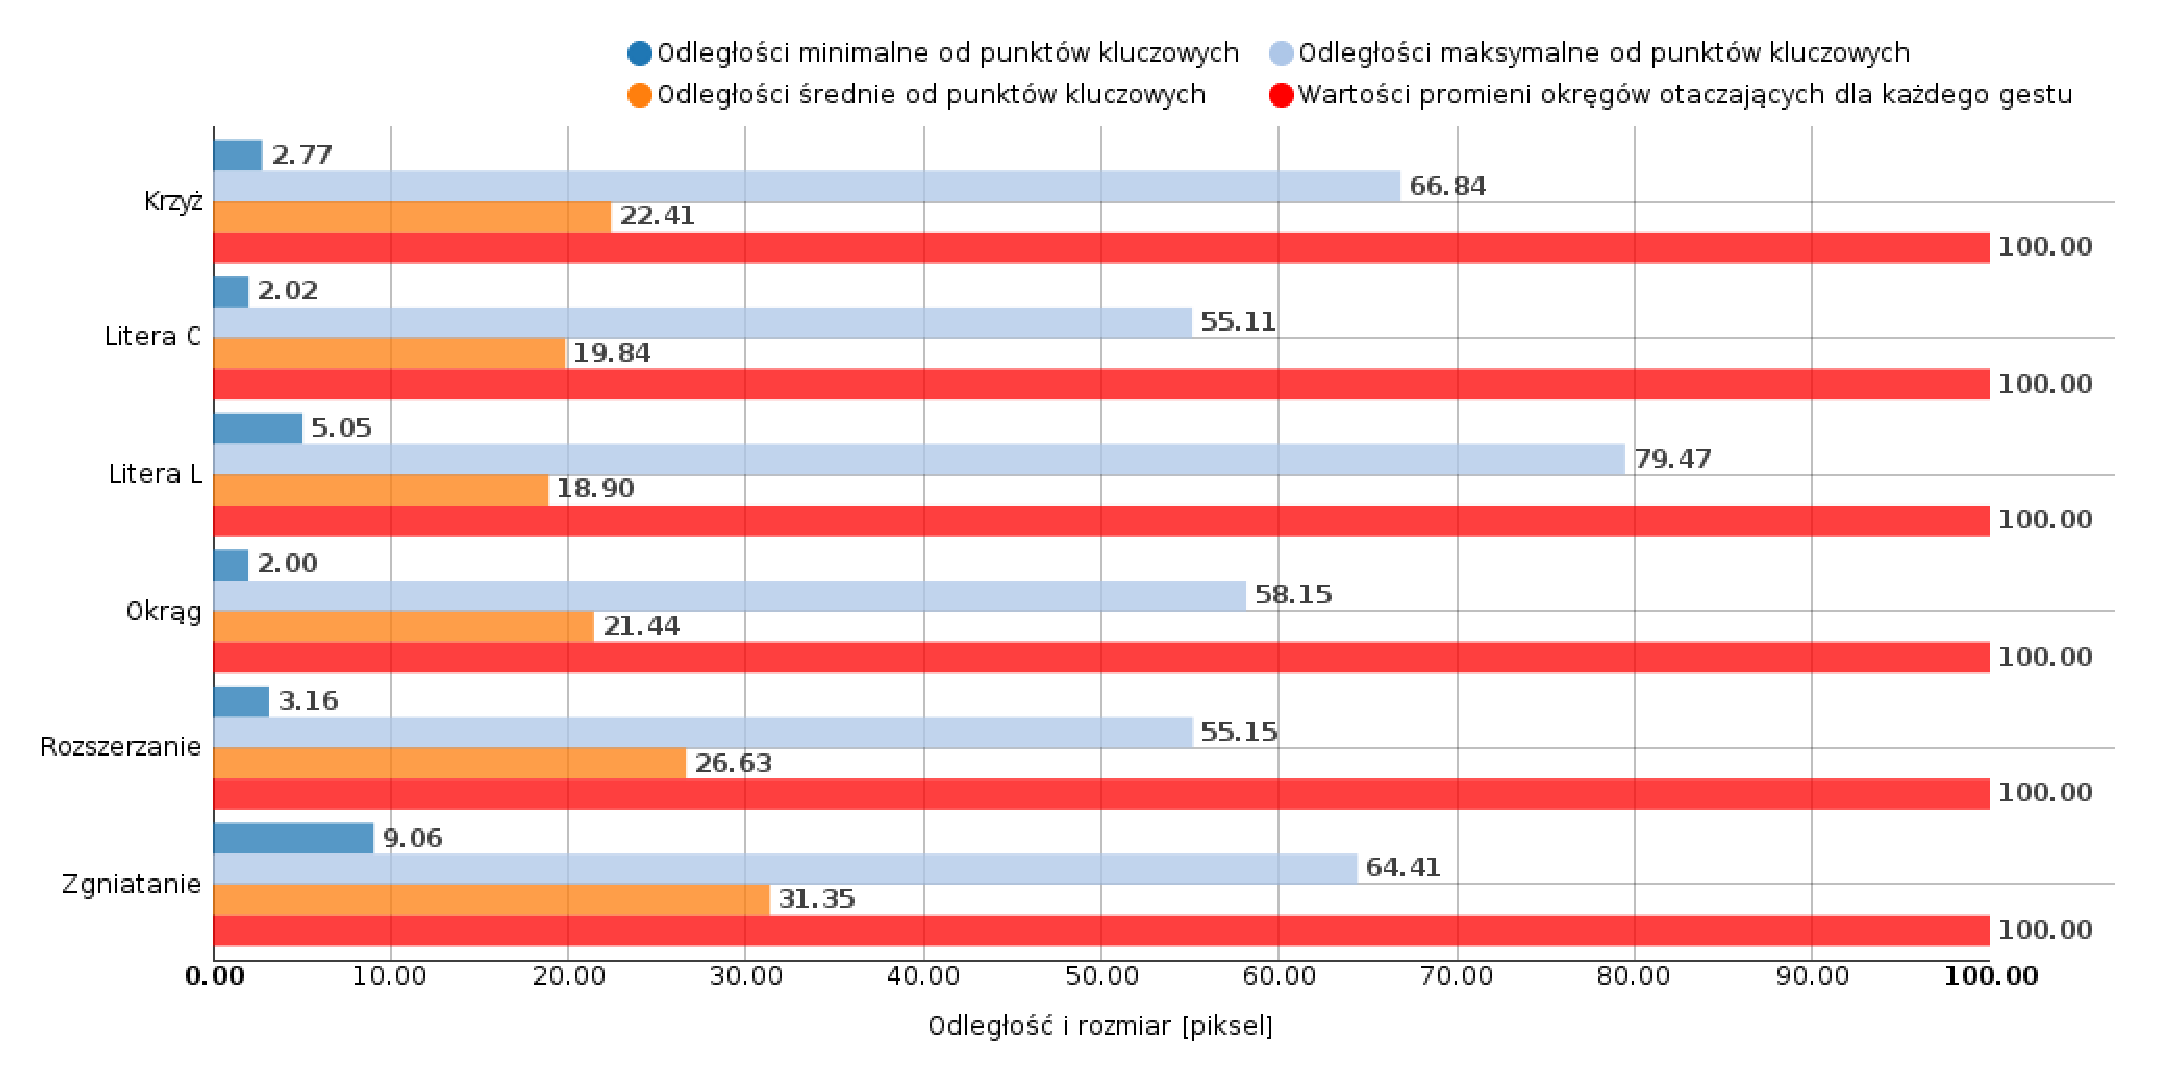
\includegraphics[width=14cm]{charts/quality/DenseKeypointsPersonG}
        \caption[Odległość od punktów wzorcowych dla każdego gestu (gęsty przepływ optyczny)]
                {Odległość od punktów wzorcowych dla każdego gestu ze zbioru G (gęsty przepływ optyczny)}
        \label{fig:DenseKeypointsPersonG}
      \end{figure}

      \begin{figure}[!ht]
        \centering
        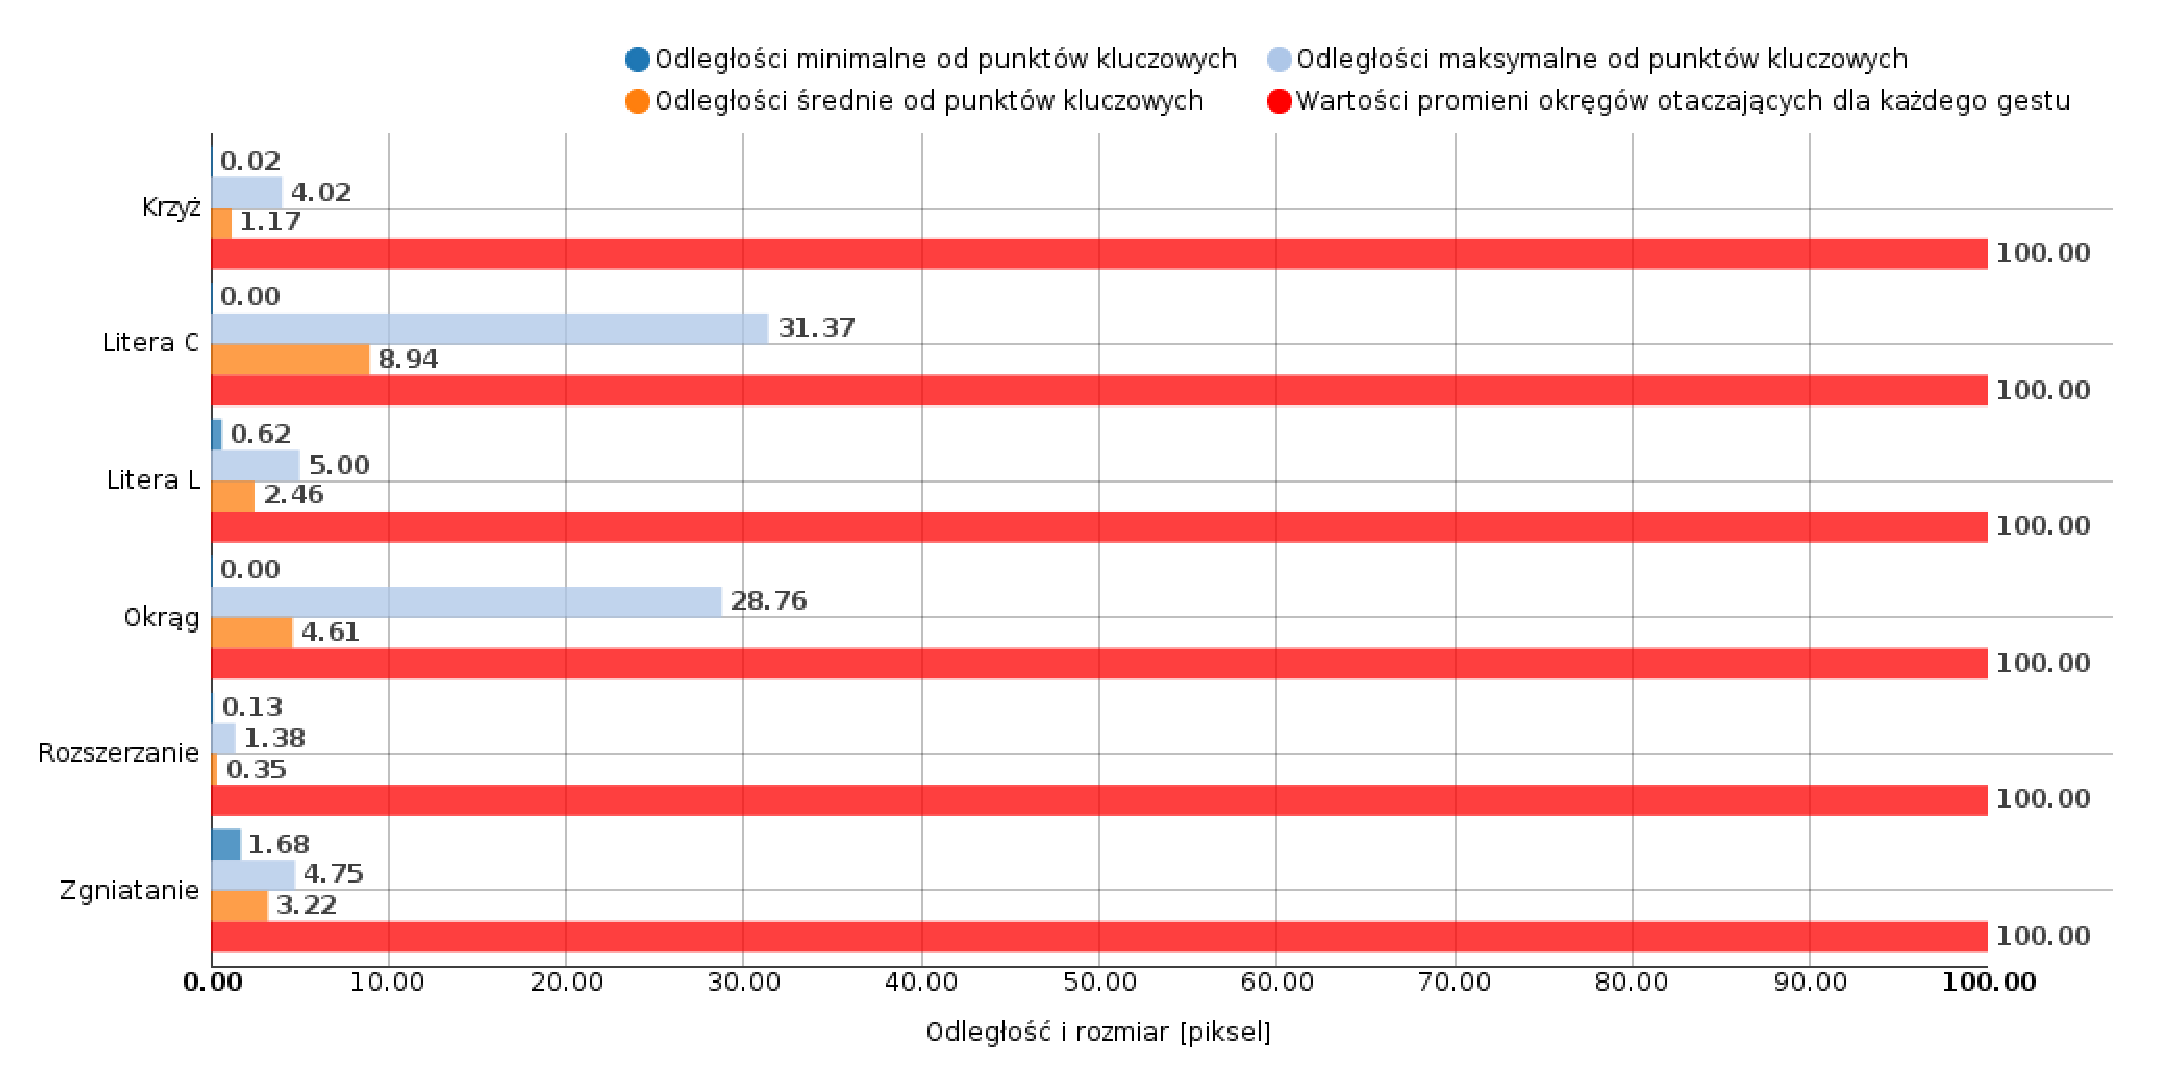
\includegraphics[width=14cm]{charts/quality/DensePathPersonG}
        \caption[Odległość od ścieżek wzorcowych dla każdego gestu (gęsty przepływ optyczny)]
                {Odległość od ścieżek wzorcowych dla każdego gestu ze zbioru G\\(gęsty przepływ optyczny)}
        \label{fig:DensePathPersonG}
      \end{figure}

    \newpage
      \begin{figure}[!ht]
        \centering
        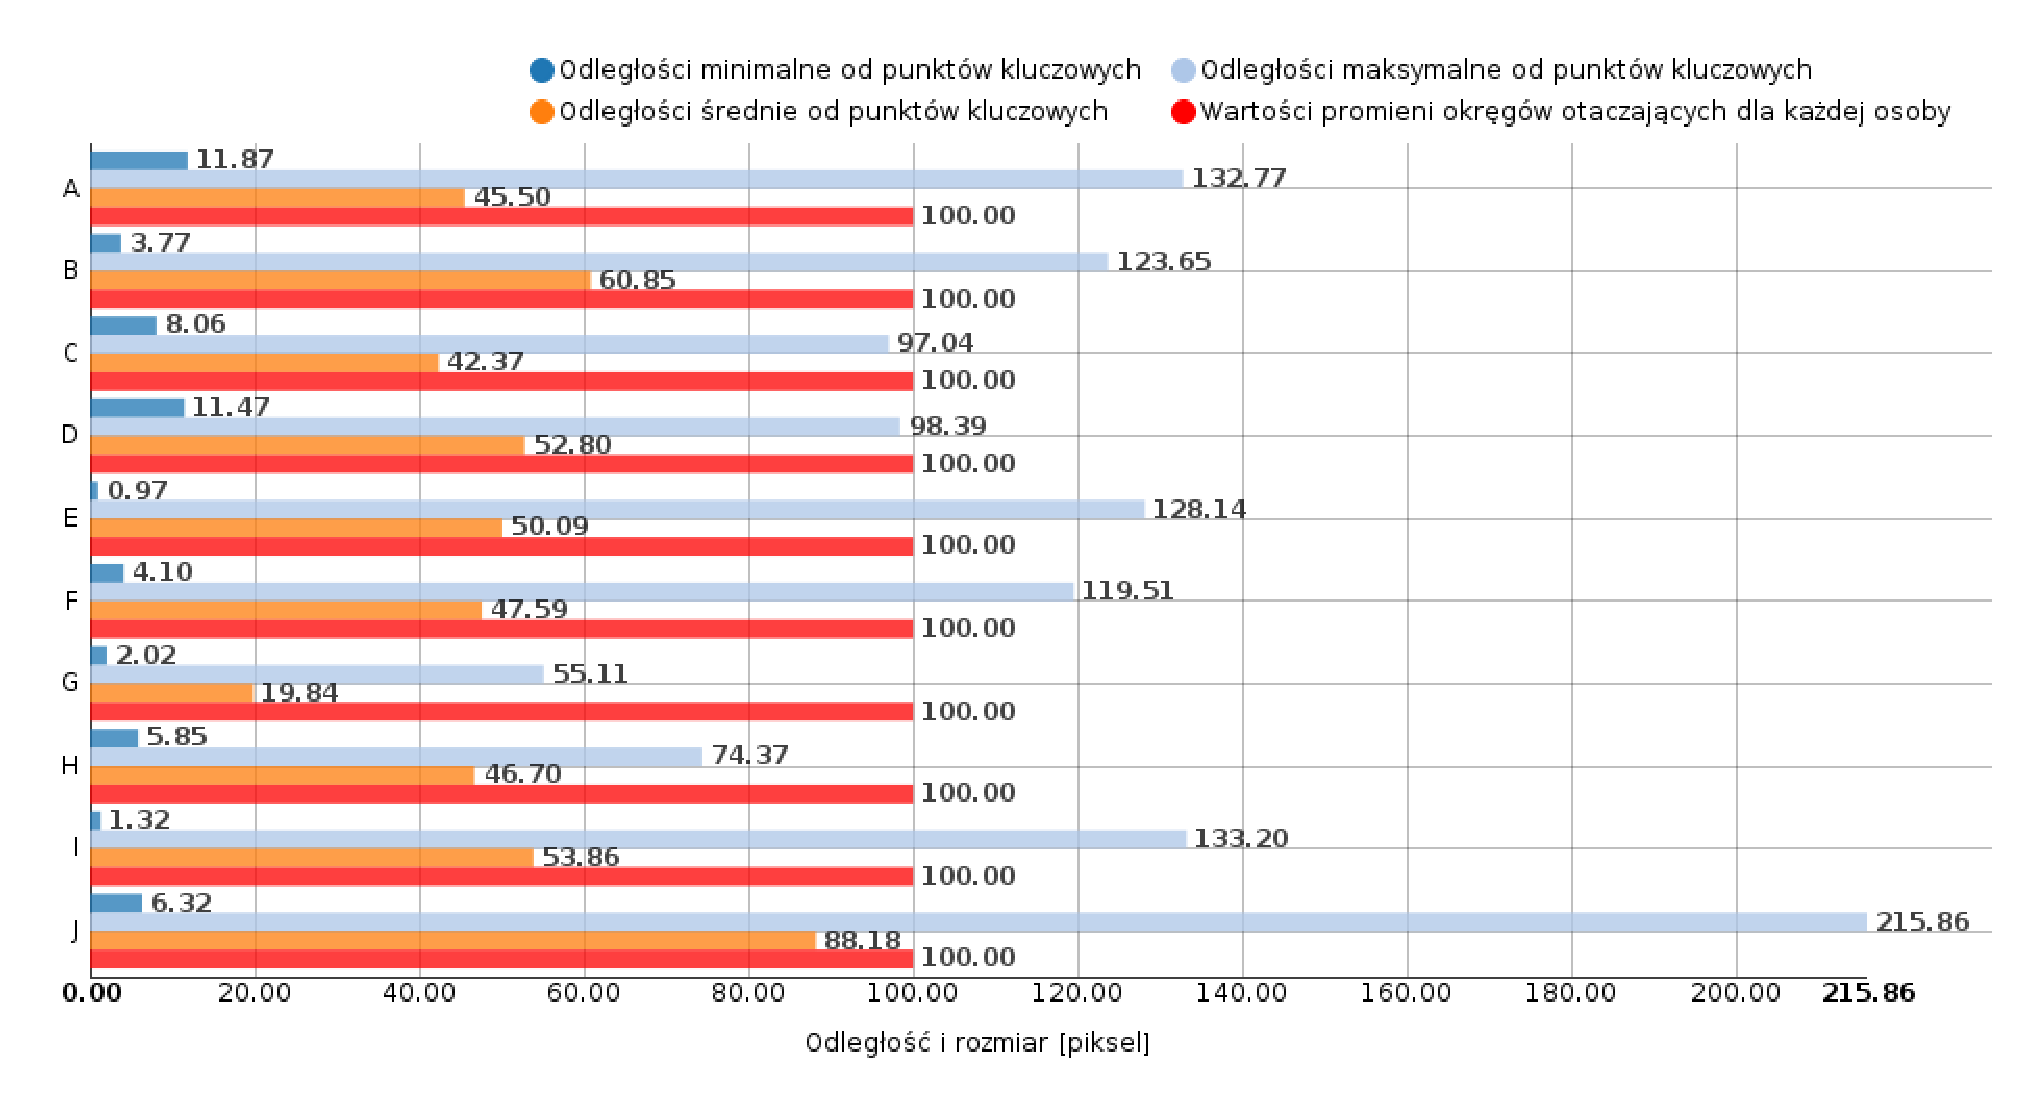
\includegraphics[width=14cm]{charts/quality/DenseKeypointsGestureC}
        \caption[Odległość od punktów wzorcowych dla każdej osoby dla gestu C (gęsty przepływ optyczny)]
                {Odległość od punktów wzorcowych dla każdej osoby dla gestu\\\textit{Wielka Litera C} (gęsty przepływ optyczny)}
        \label{fig:DenseKeypointsGestureC}
      \end{figure}

      \begin{figure}[!ht]
        \centering
        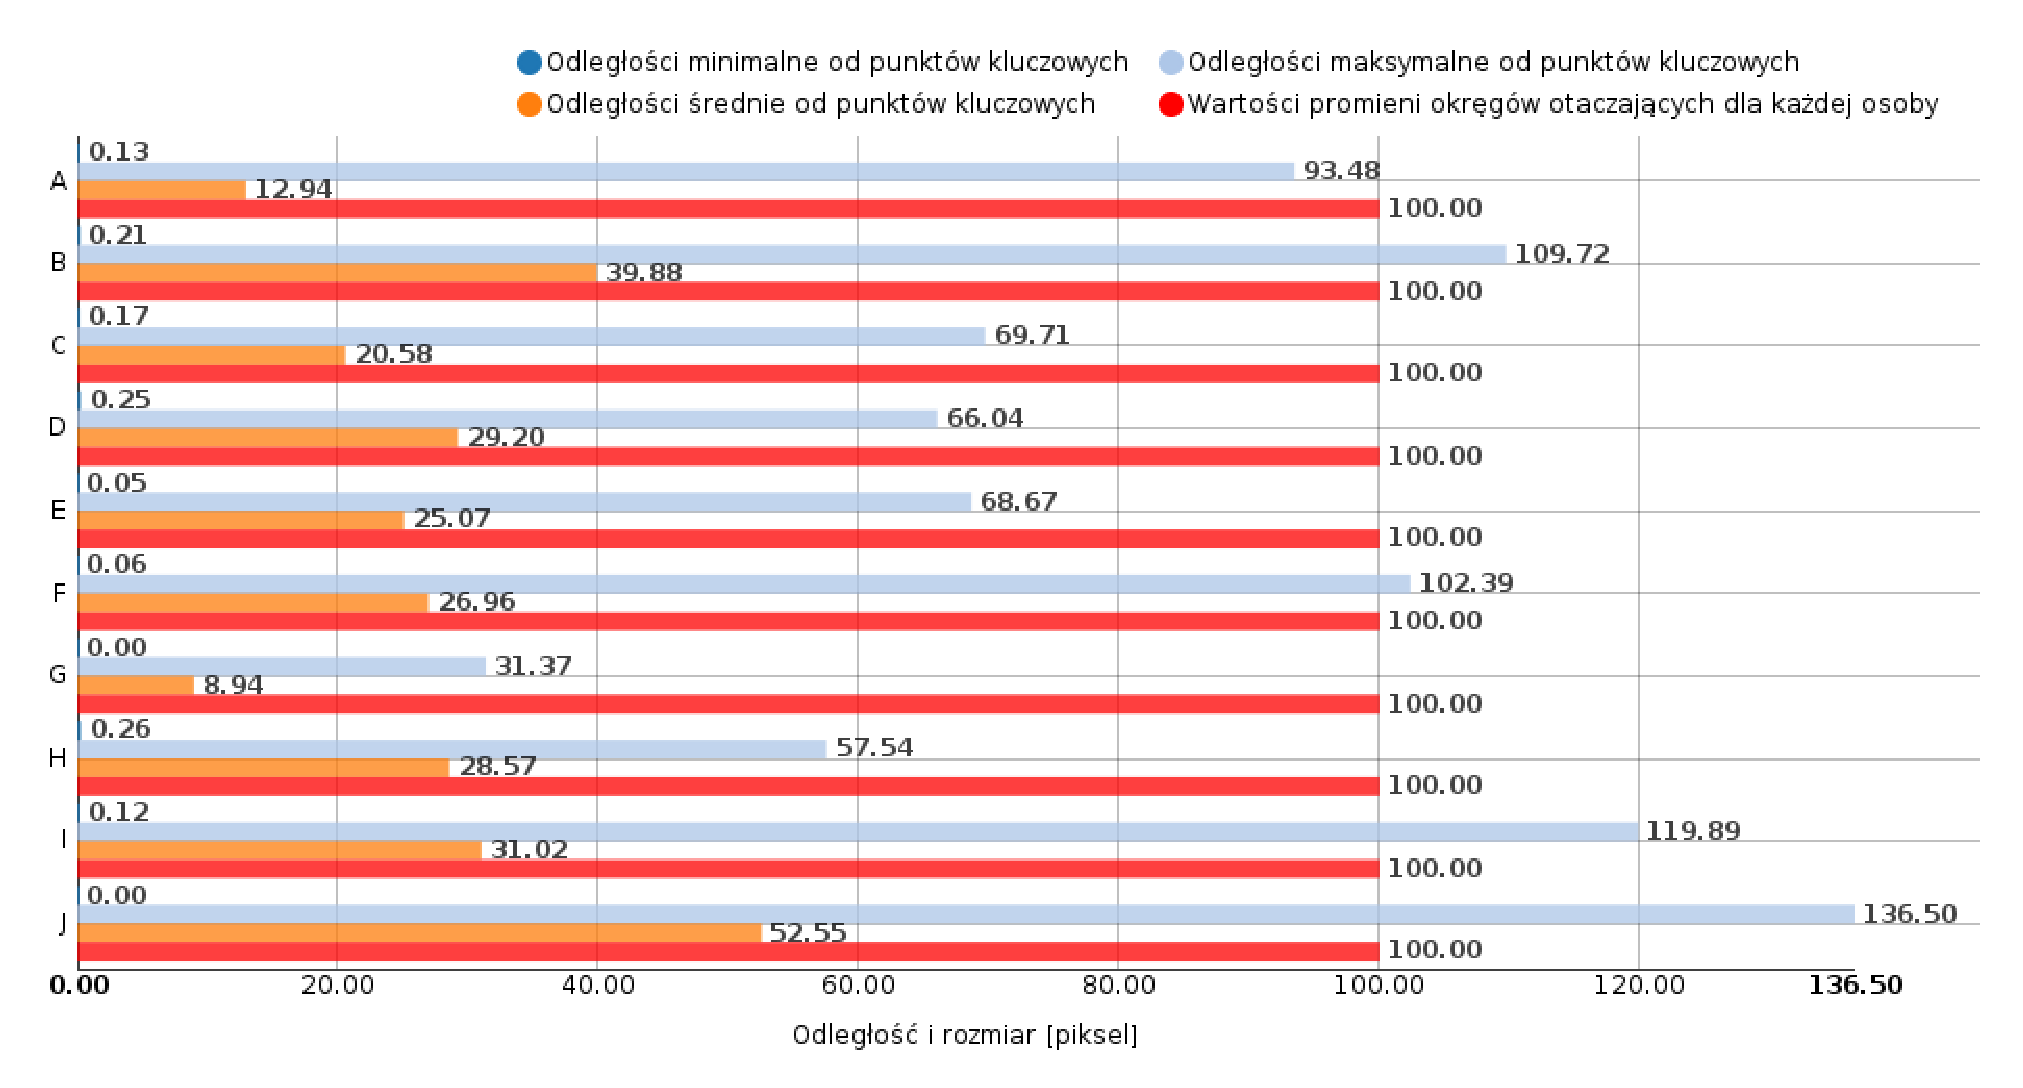
\includegraphics[width=14cm]{charts/quality/DensePathGestureC}
        \caption[Odległość od ścieżek wzorcowych dla każdej osoby dla gestu C (gęsty przepływ optyczny)]
                {Odległość od ścieżek wzorcowych dla każdej osoby dla gestu\\\textit{Wielka Litera C} (gęsty przepływ optyczny)}
        \label{fig:DensePathGestureC}
      \end{figure}

    \newpage
      \begin{figure}[!ht]
        \centering
        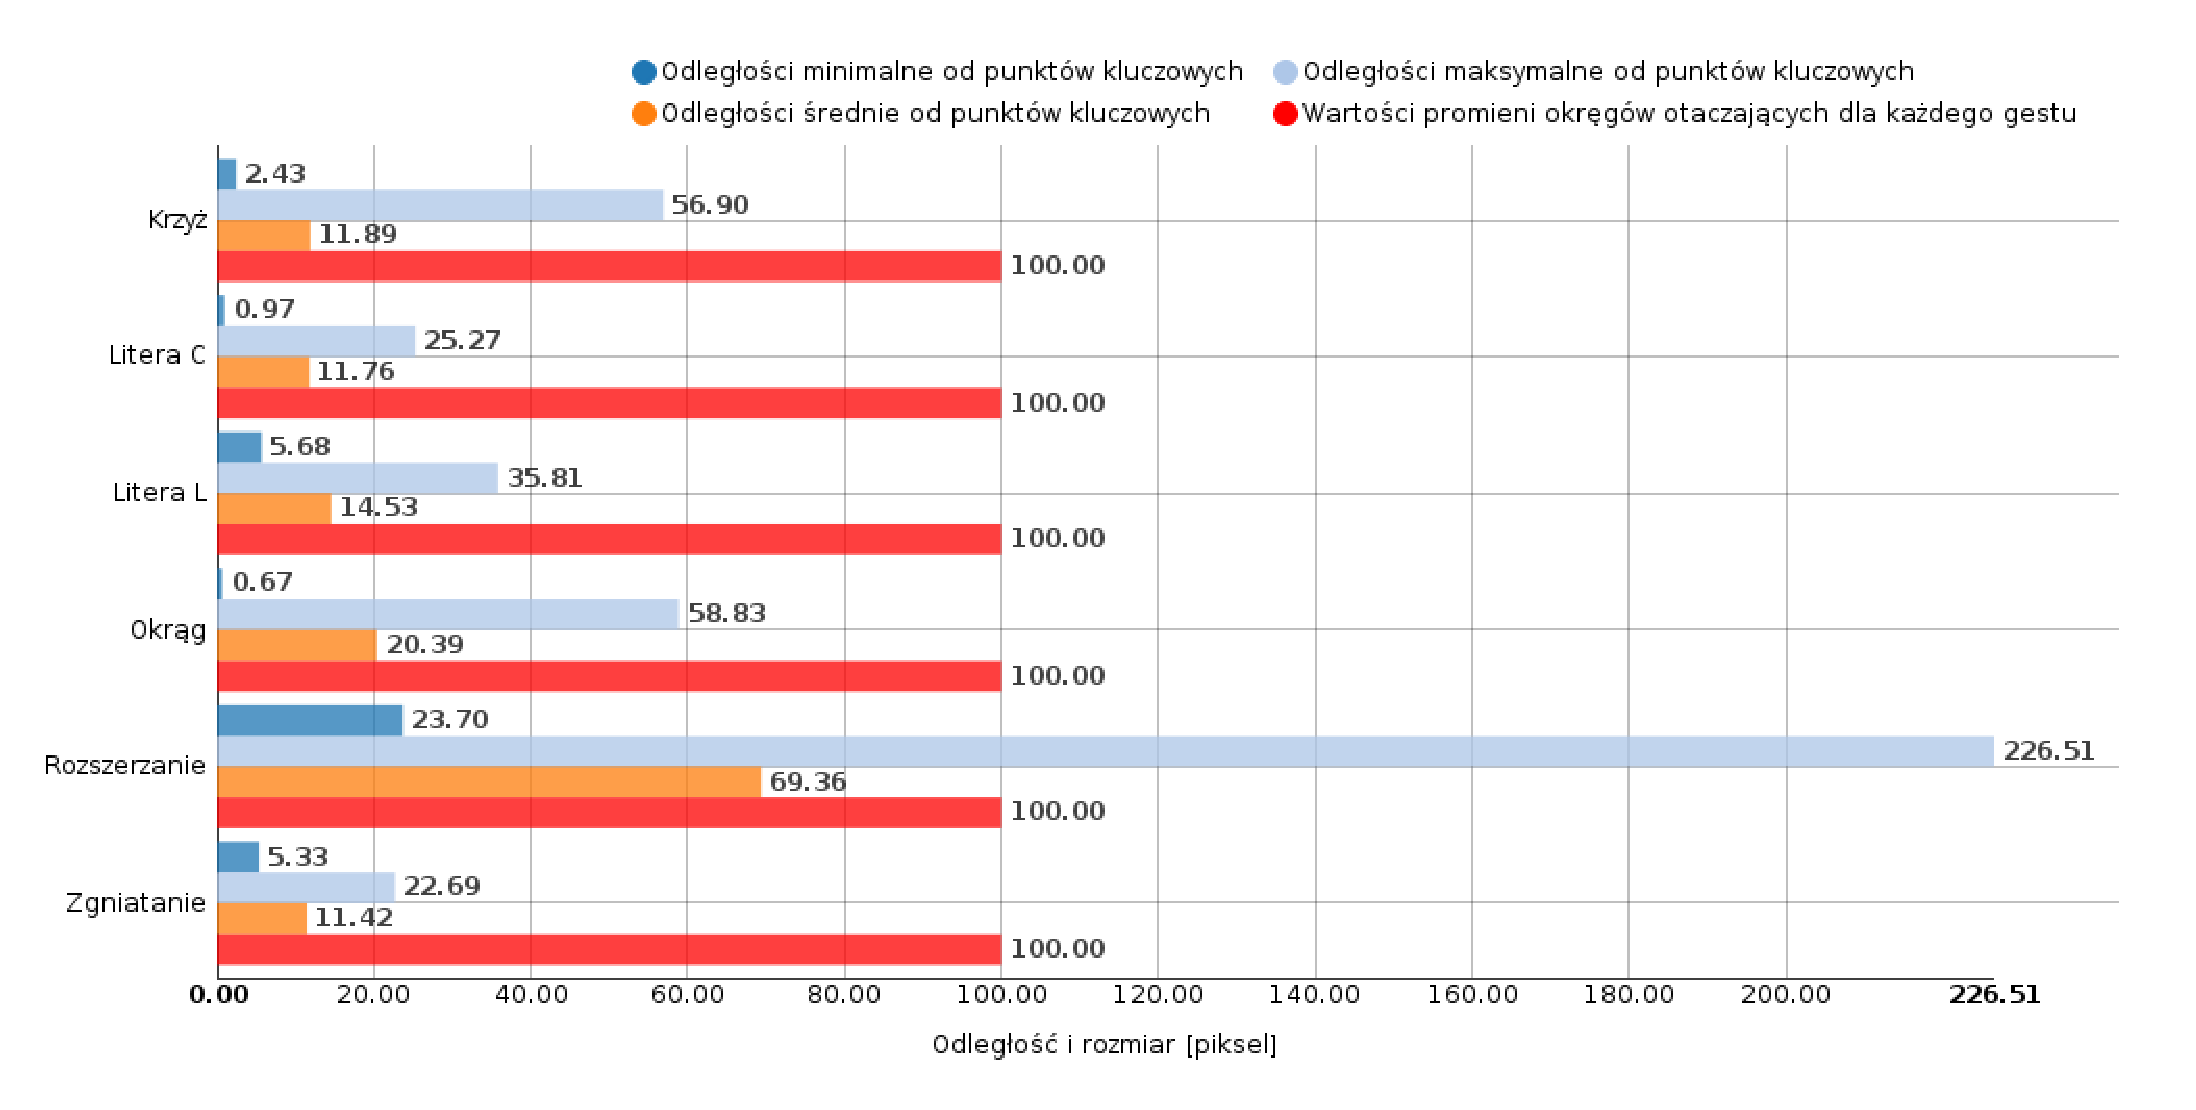
\includegraphics[width=14cm]{charts/quality/RandomKeypointsPersonG}
        \caption[Odległość od punktów wzorcowych dla każdego gestu (las drzew losowych)]
                {Odległość od punktów wzorcowych dla każdego gestu ze zbioru G\\(las drzew losowych)}
        \label{fig:RandomKeypointsPersonG}
      \end{figure}

      \begin{figure}[!ht]
        \centering
        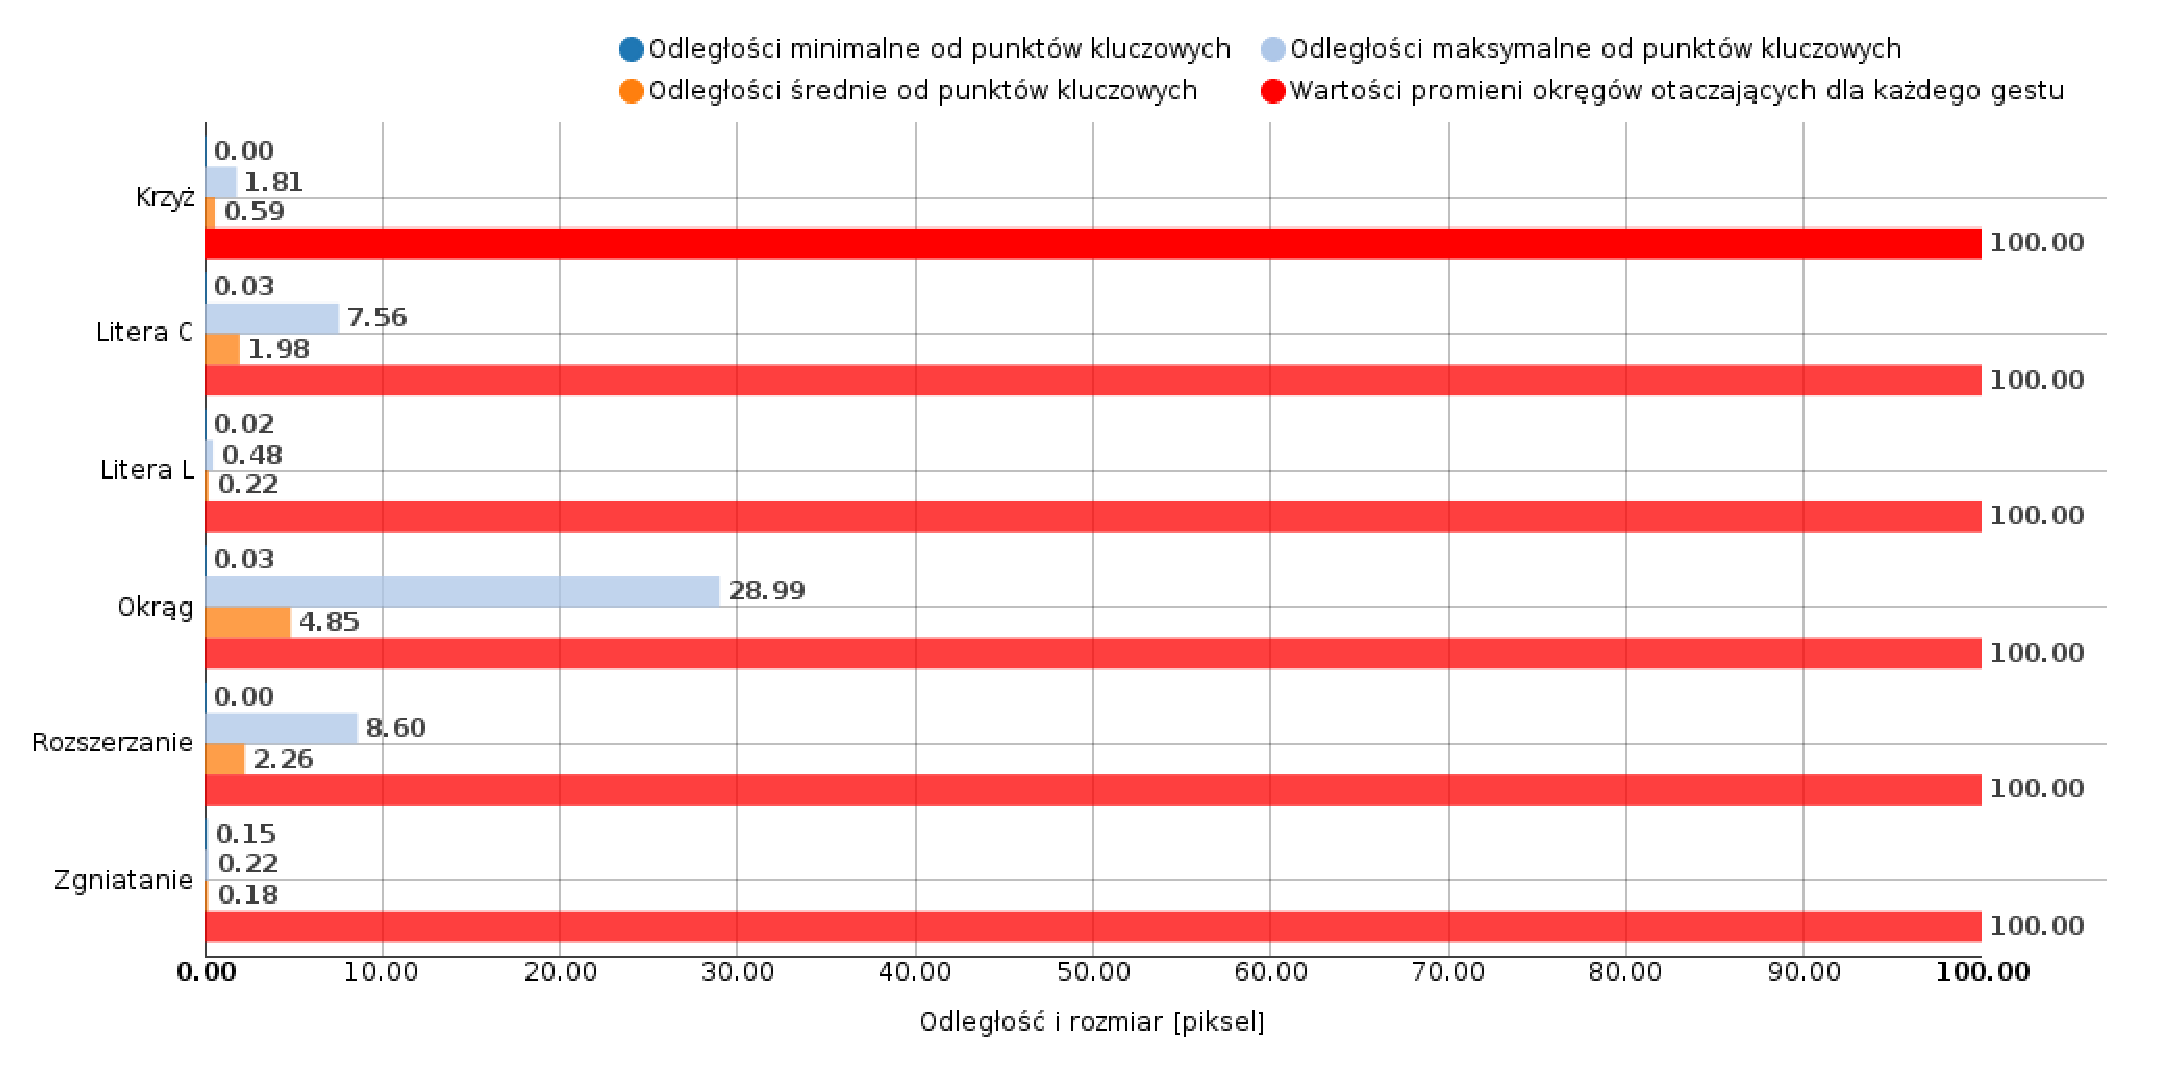
\includegraphics[width=14cm]{charts/quality/RandomPathPersonG}
        \caption[Odległość od ścieżek wzorcowych dla każdego gestu (las drzew losowych)]
                {Odległość od ścieżek wzorcowych dla każdego gestu ze zbioru G\\(las drzew losowych)}
        \label{fig:RandomPathPersonG}
      \end{figure}

    \newpage
      \begin{figure}[!ht]
        \centering
        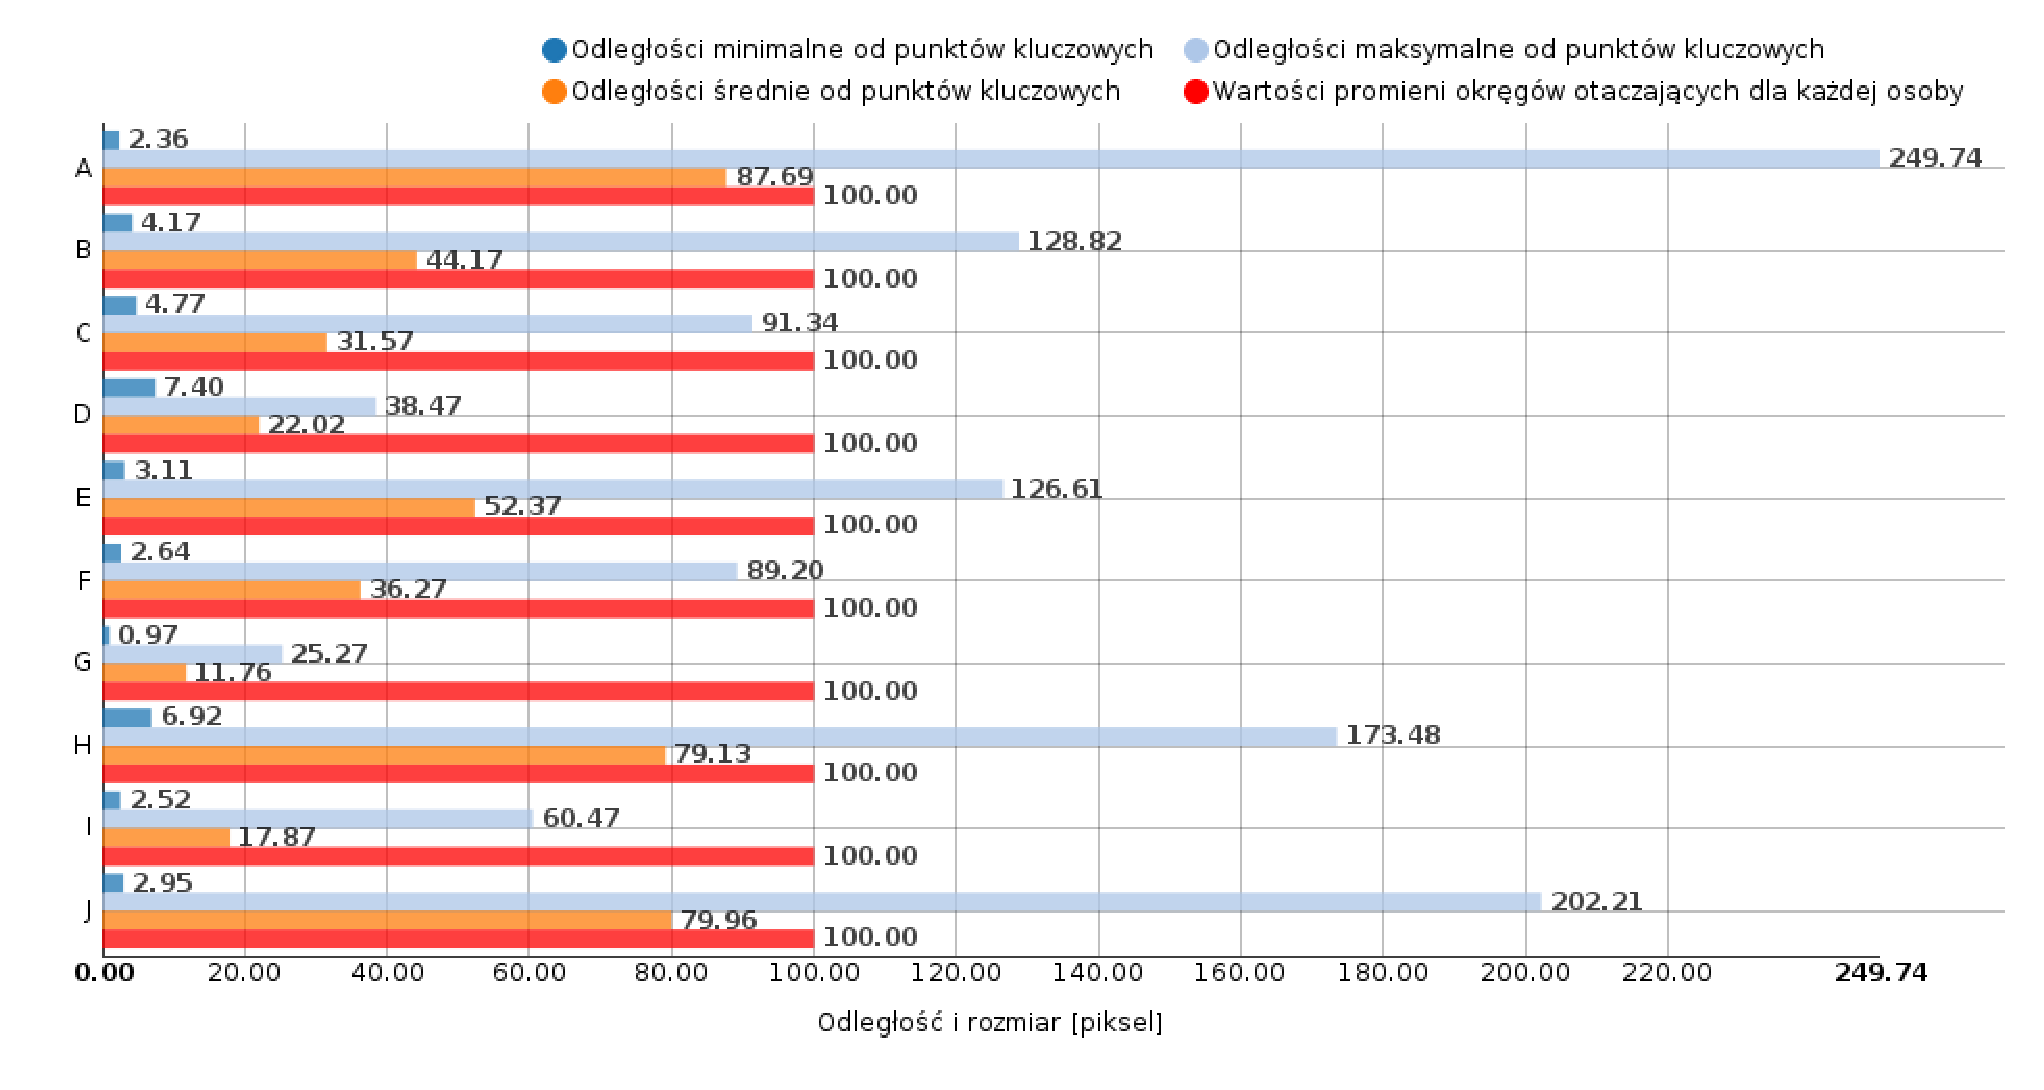
\includegraphics[width=14cm]{charts/quality/RandomKeypointsGestureC}
        \caption[Odległość od punktów wzorcowych dla każdej osoby dla gestu C (las drzew losowych)]
                {Odległość od punktów wzorcowych dla każdej osoby dla gestu\\
                 \textit{Wielka Litera C} (las drzew losowych)}
        \label{fig:RandomKeypointsGestureC}
      \end{figure}

      \begin{figure}[!ht]
        \centering
        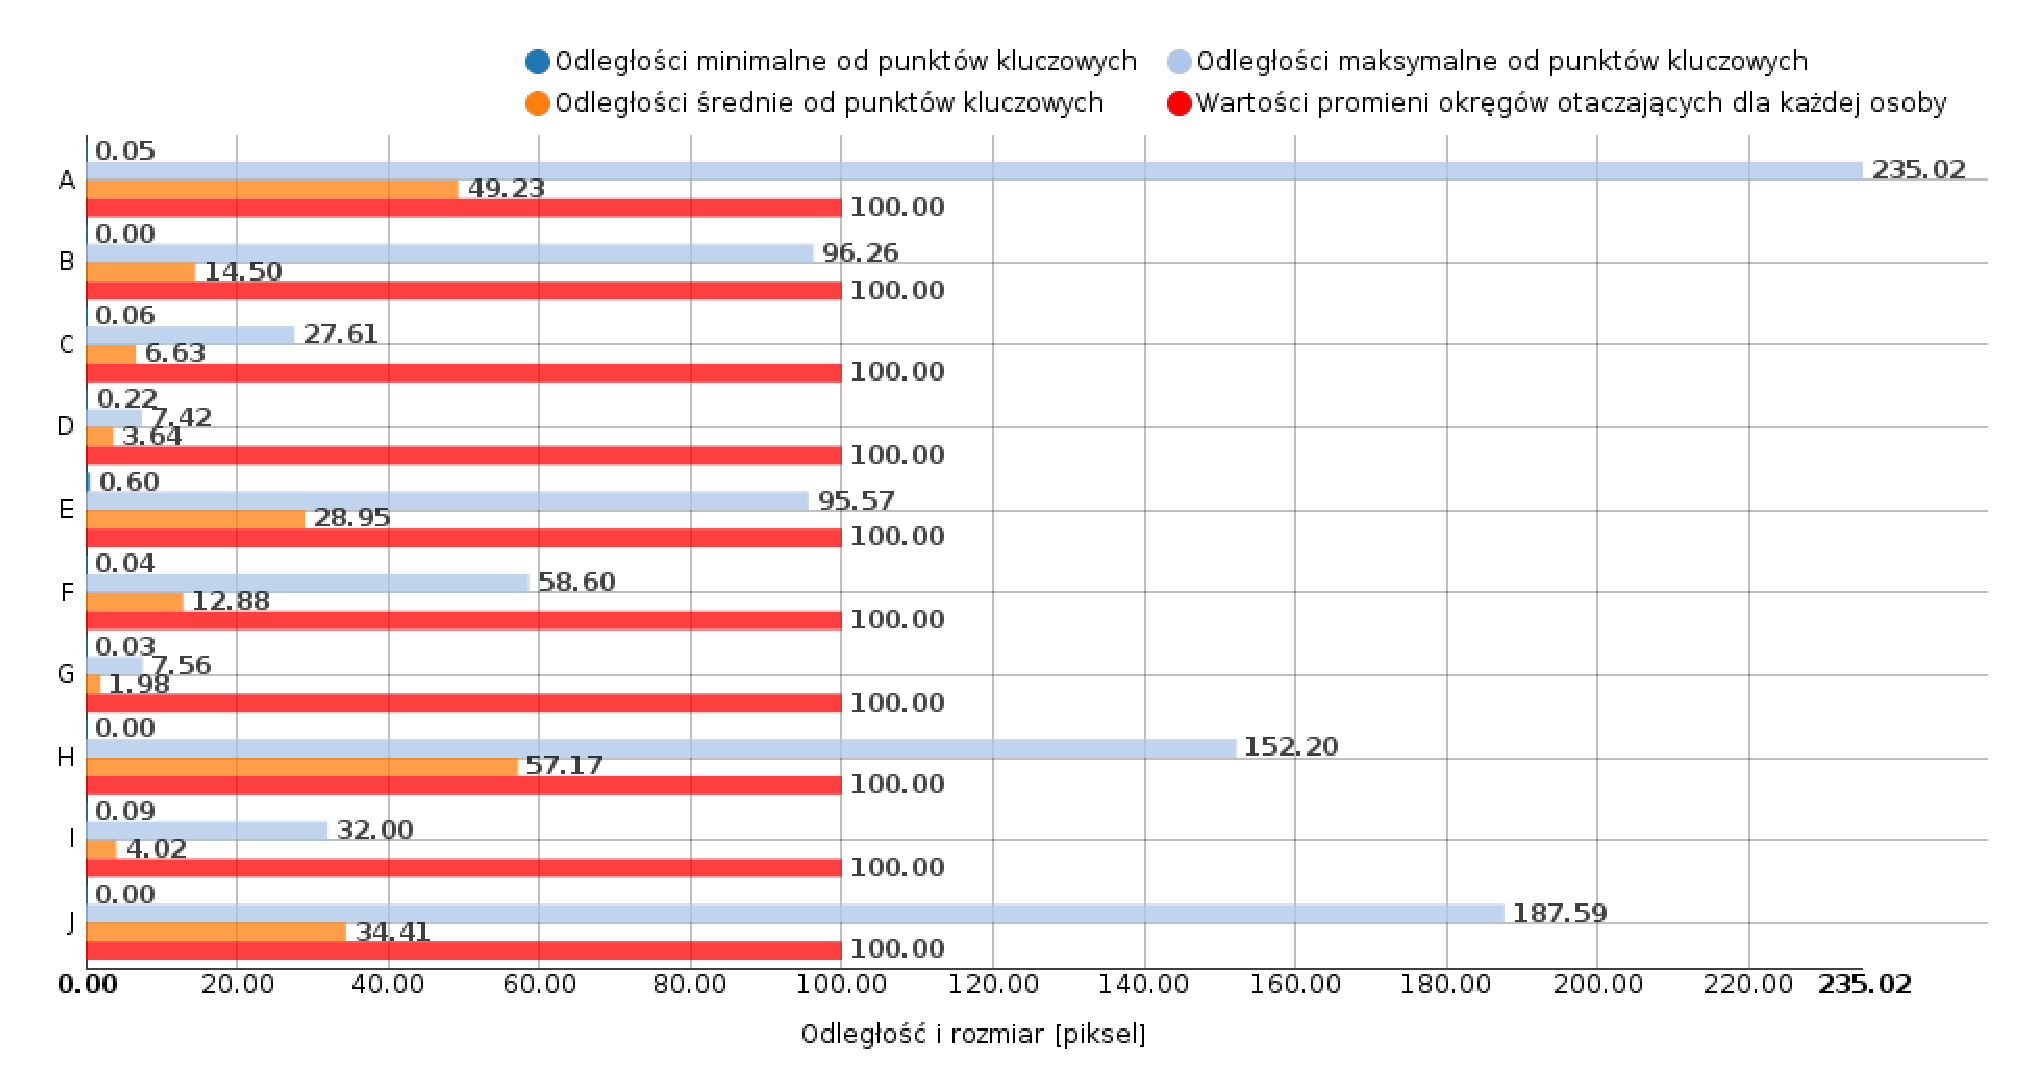
\includegraphics[width=14cm]{charts/quality/RandomPathGestureC}
        \caption[Odległość od ścieżek wzorcowych dla każdej osoby dla gestu C (las drzew losowych)]
                {Odległość od ścieżek wzorcowych dla każdej osoby dla gestu\\
                 \textit{Wielka Litera C} (las drzew losowych)}
        \label{fig:RandomPathGestureC}
      \end{figure}

    \newpage
      \begin{figure}[!ht]
        \centering
        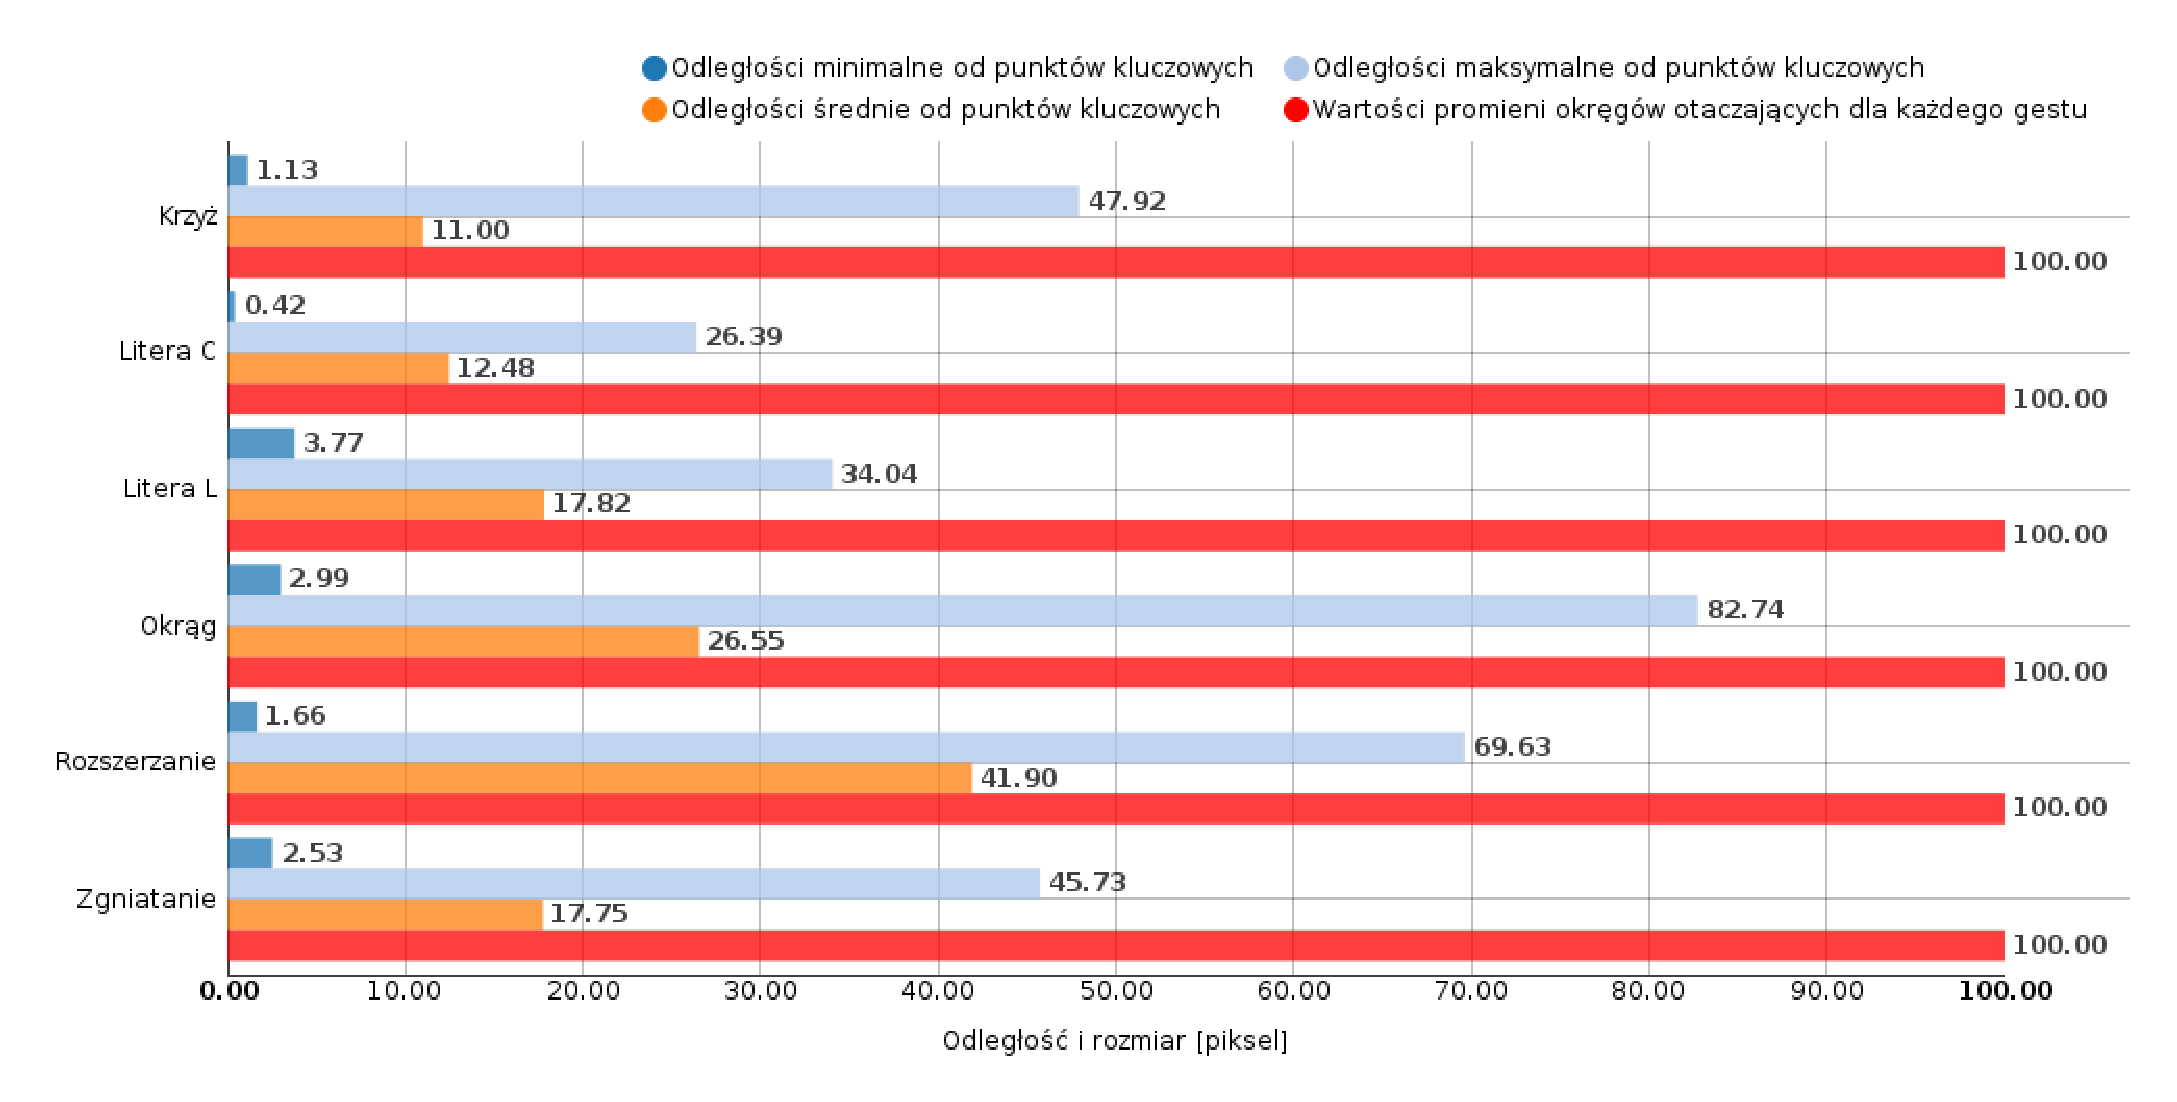
\includegraphics[width=14cm]{charts/quality/SparseKeypointsPersonG}
        \caption[Odległość od punktów wzorcowych dla każdego gestu (rzadki przepływ optyczny)]
                {Odległość od punktów wzorcowych dla każdego gestu ze zbioru G\\(rzadki przepływ optyczny)}
        \label{fig:SparseKeypointsPersonG}
      \end{figure}

      \begin{figure}[!ht]
        \centering
        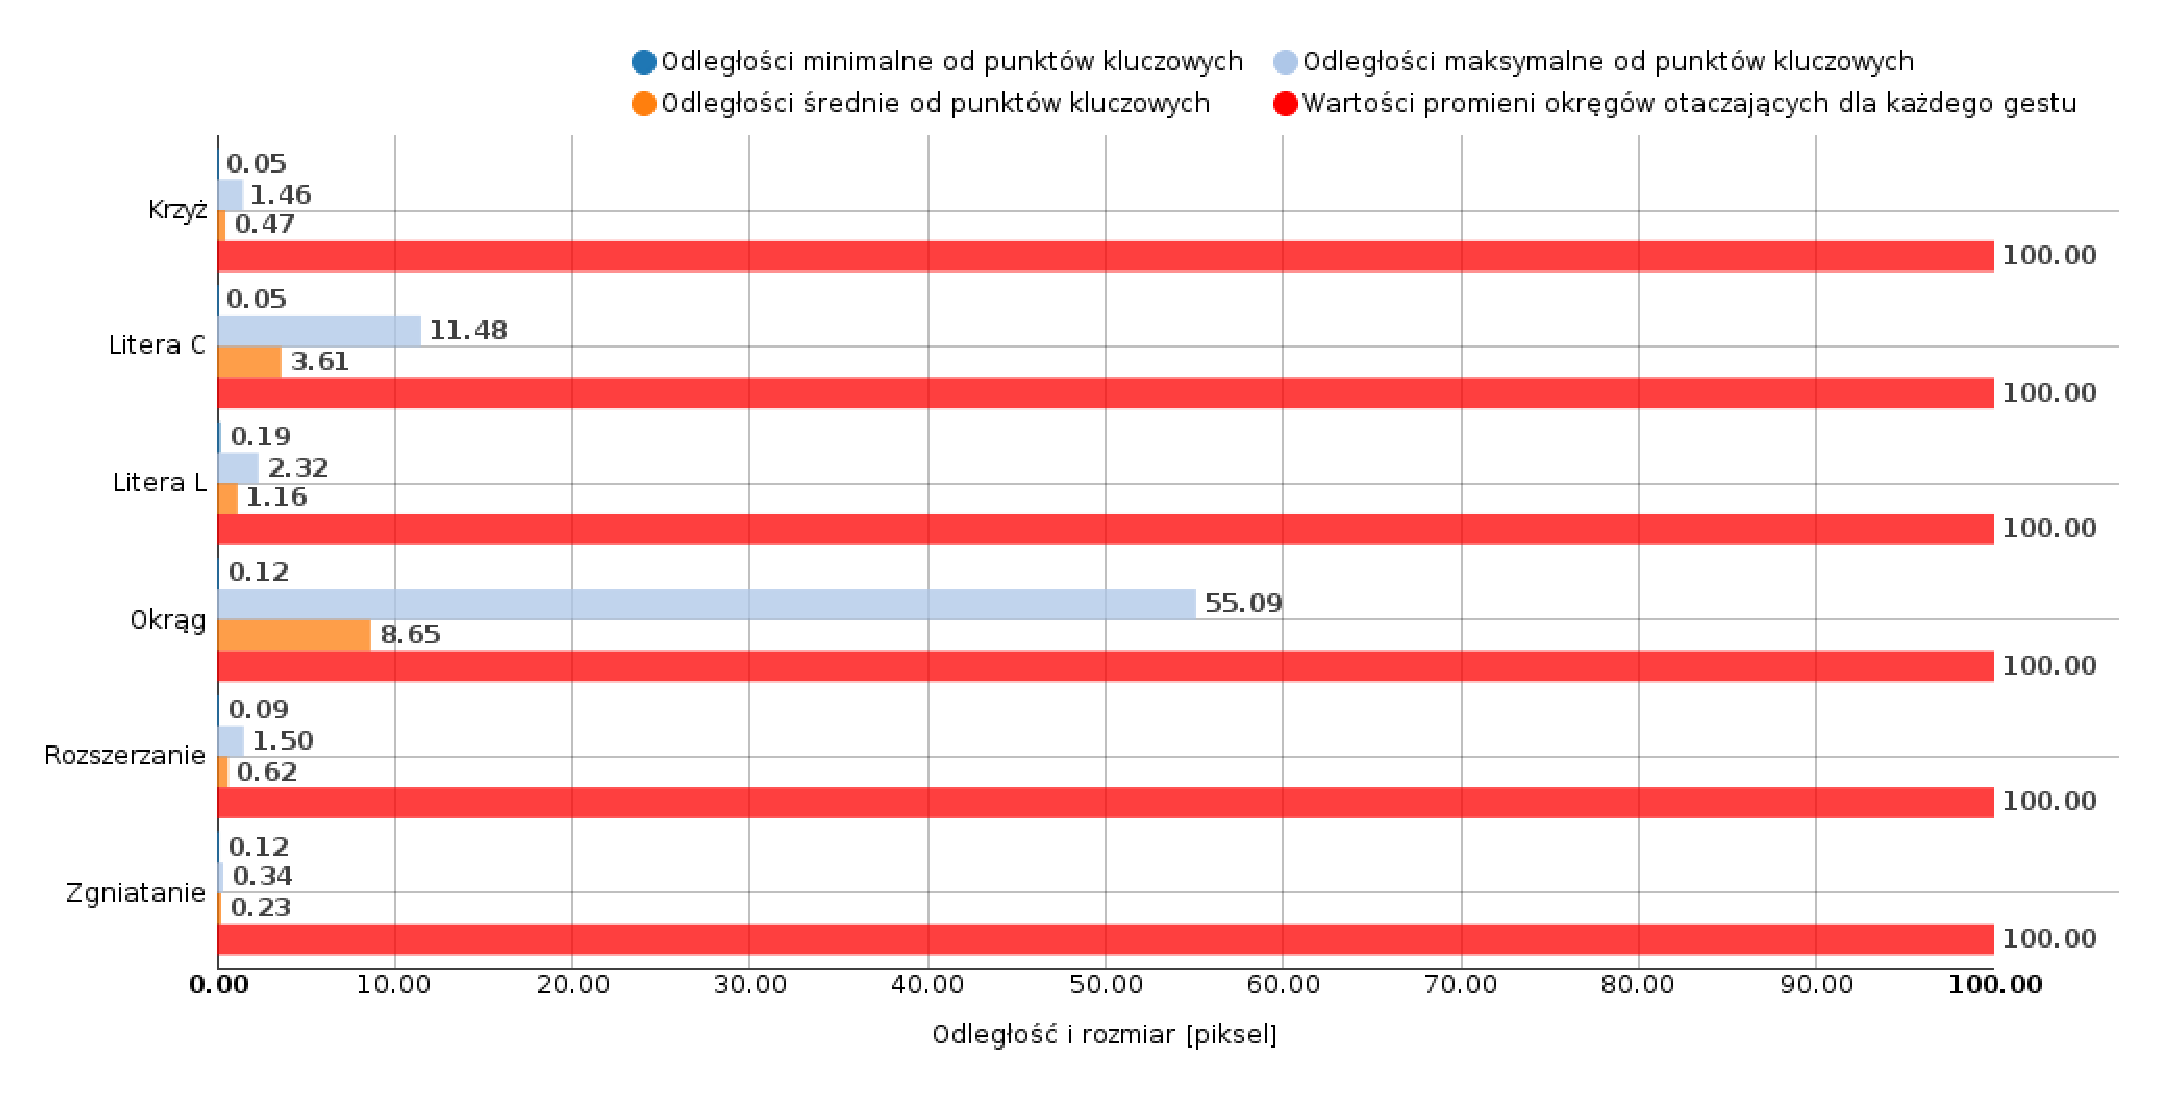
\includegraphics[width=14cm]{charts/quality/SparsePathPersonG}
        \caption[Odległość od ścieżek wzorcowych dla każdego gestu (rzadki przepływ optyczny)]
                {Odległość od ścieżek wzorcowych dla każdego gestu ze zbioru G\\(rzadki przepływ optyczny)}
        \label{fig:SparsePathPersonG}
      \end{figure}

    \newpage
      \begin{figure}[!ht]
        \centering
        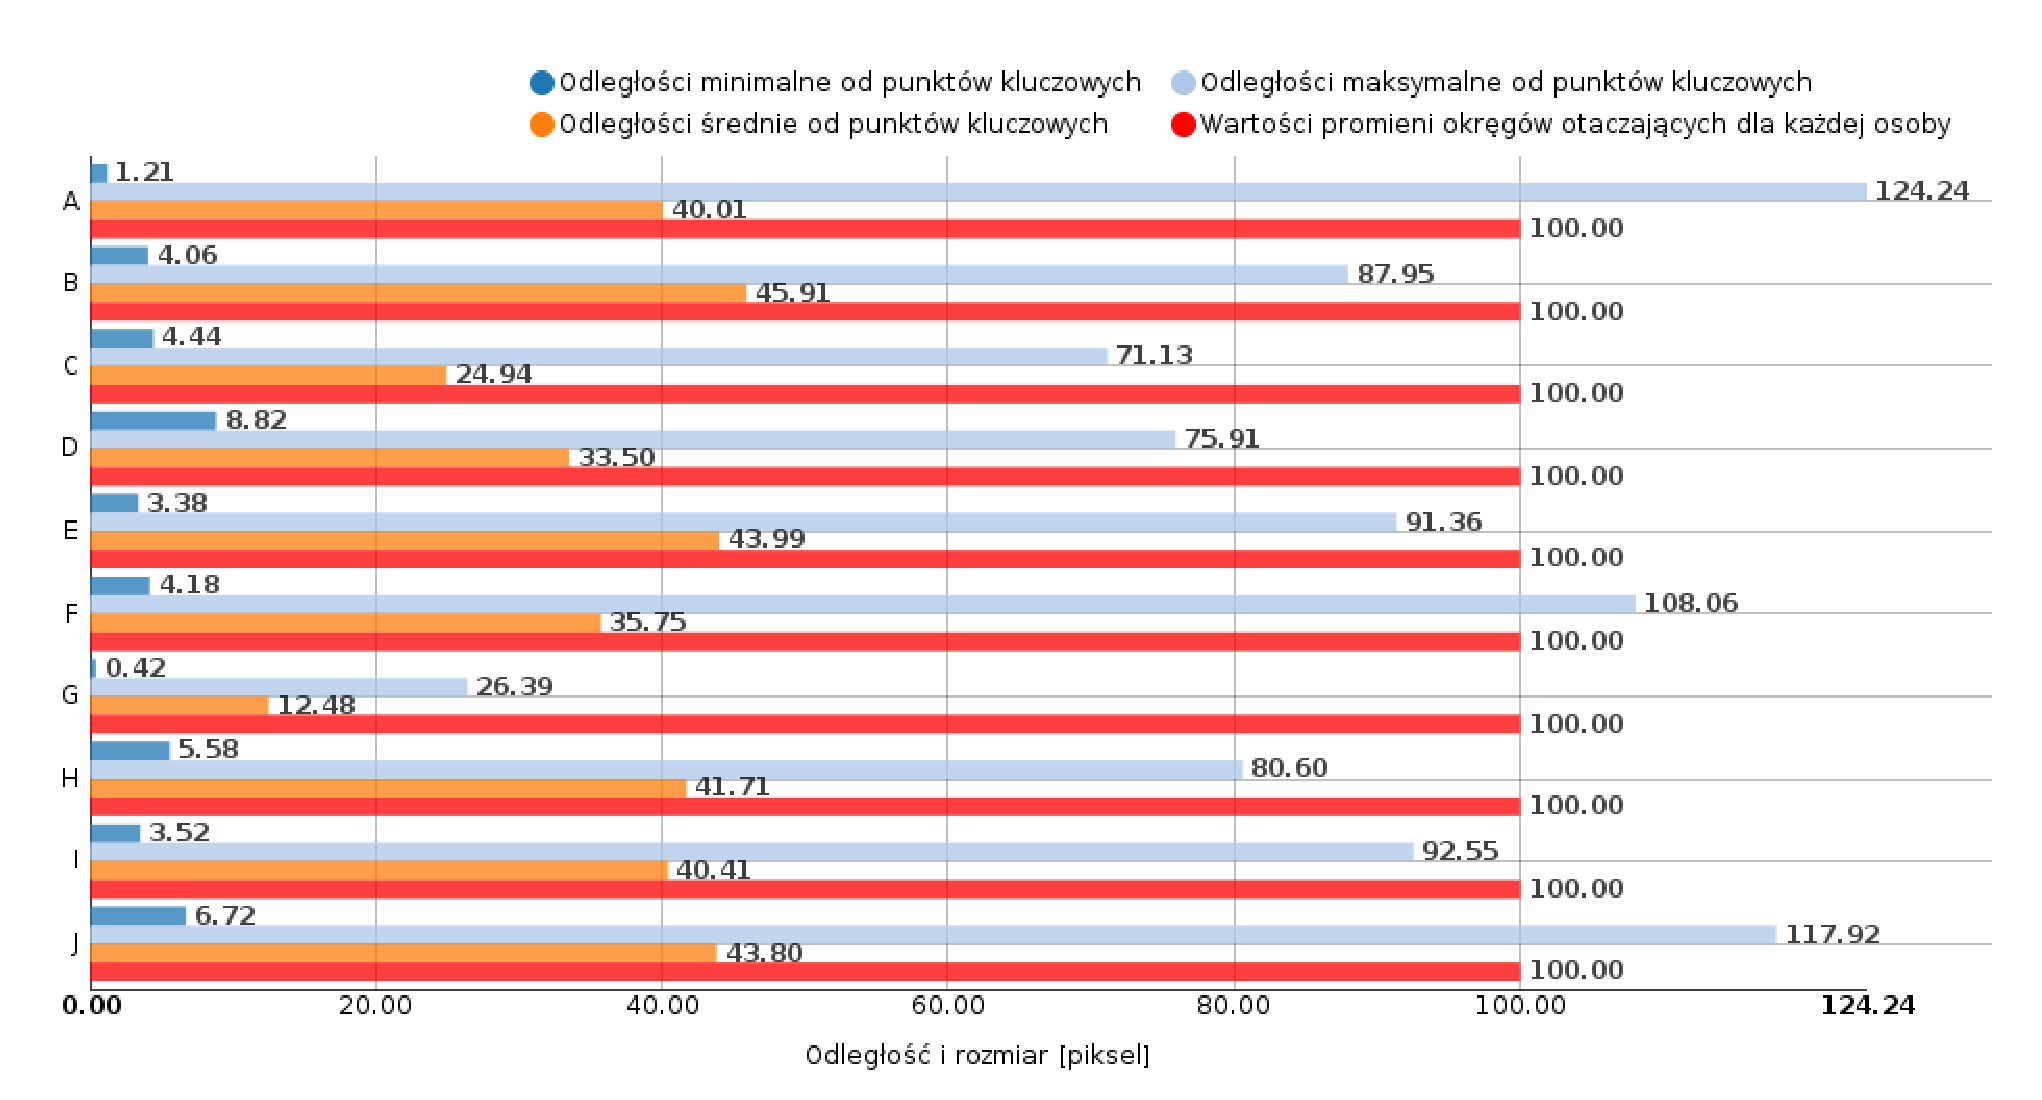
\includegraphics[width=14cm]{charts/quality/SparseKeypointsGestureC}
        \caption[Odległość od punktów wzorcowych dla każdej osoby dla gestu C (rzadki przepływ optyczny)]
                {Odległość od punktów wzorcowych dla każdej osoby dla gestu\\\textit{Wielka Litera C} (rzadki przepływ optyczny)}
        \label{fig:SparseKeypointsGestureC}
      \end{figure}

      \begin{figure}[!ht]
        \centering
        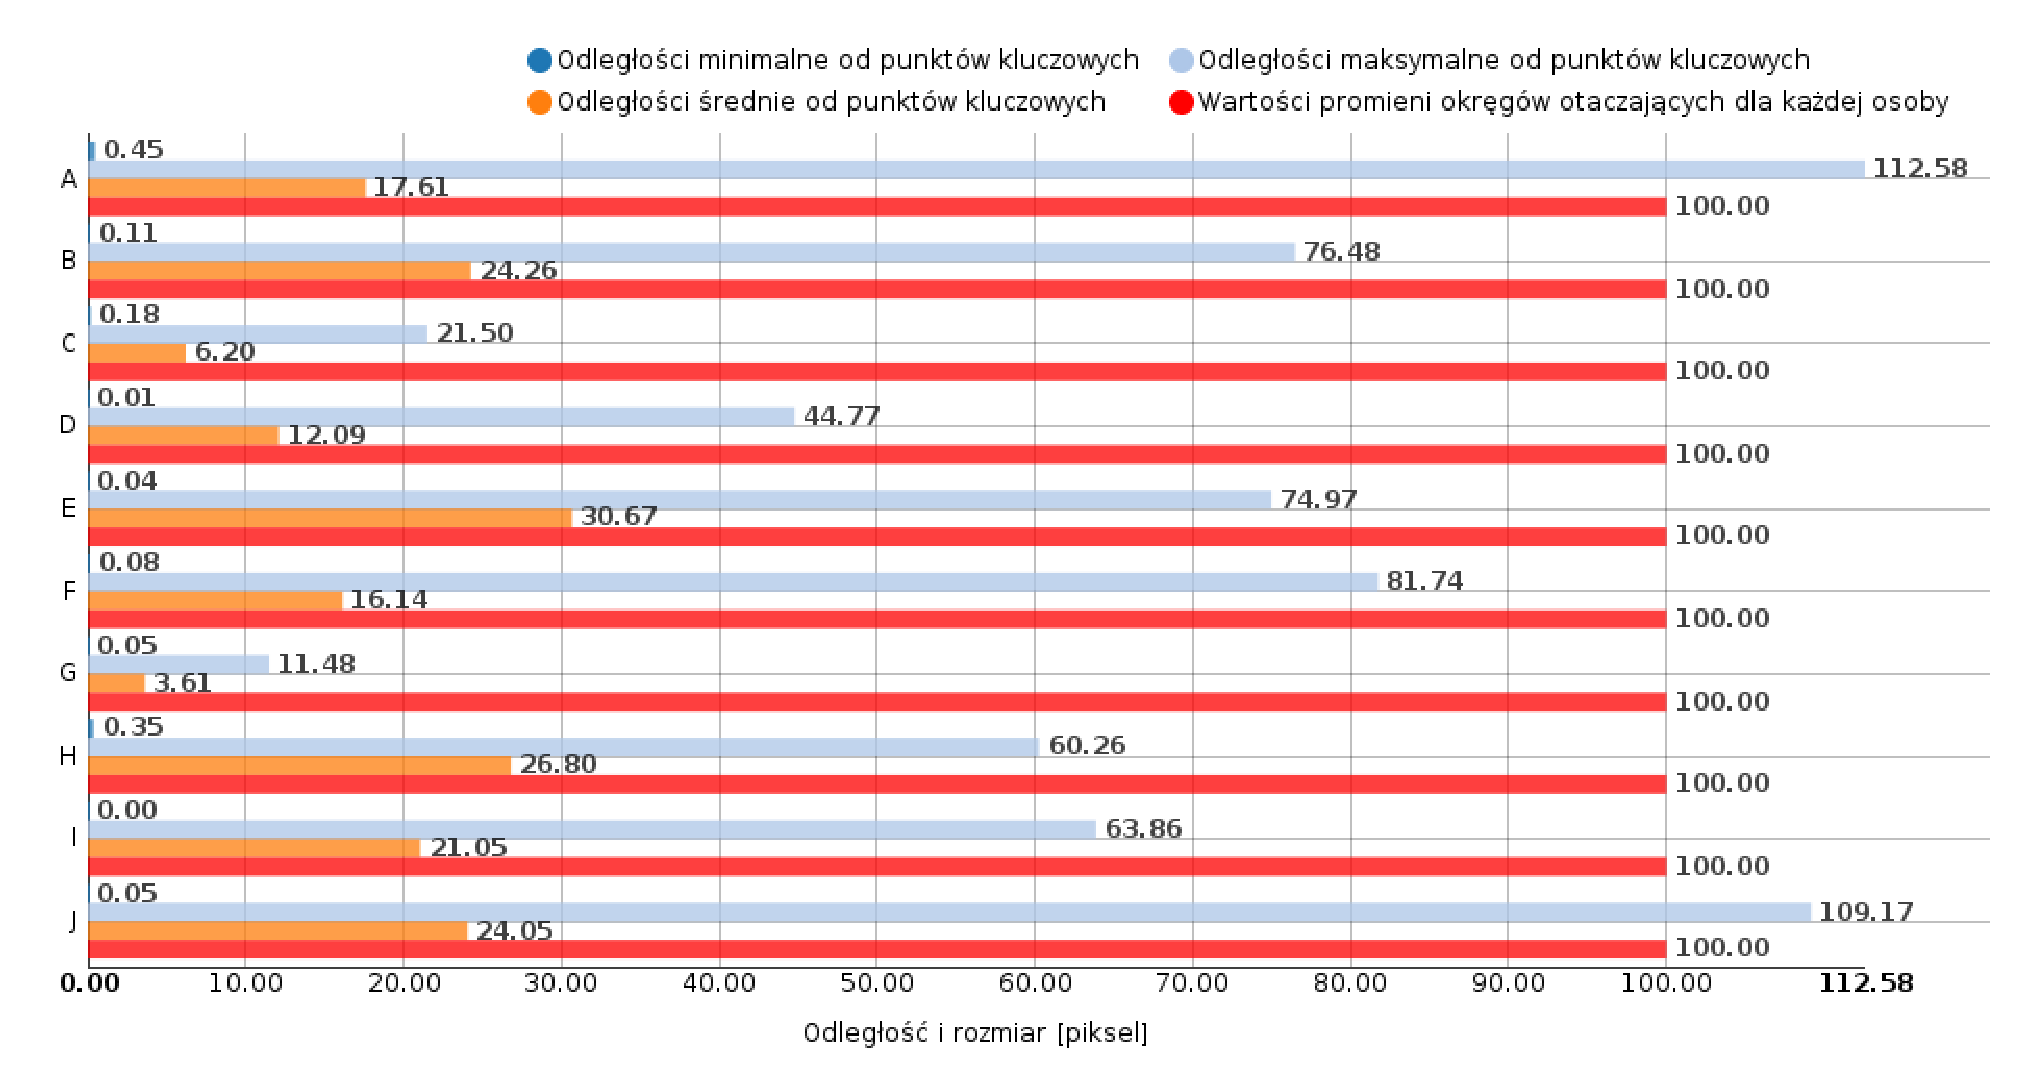
\includegraphics[width=14cm]{charts/quality/SparsePathGestureC}
        \caption[Odległość od ścieżek wzorcowych dla każdej osoby dla gestu C (rzadki przepływ optyczny)]
                {Odległość od ścieżek wzorcowych dla każdej osoby dla gestu\\\textit{Wielka Litera C} (rzadki przepływ optyczny)}
        \label{fig:SparsePathGestureC}
      \end{figure}

    \newpage
      \begin{figure}[!ht]
        \centering
        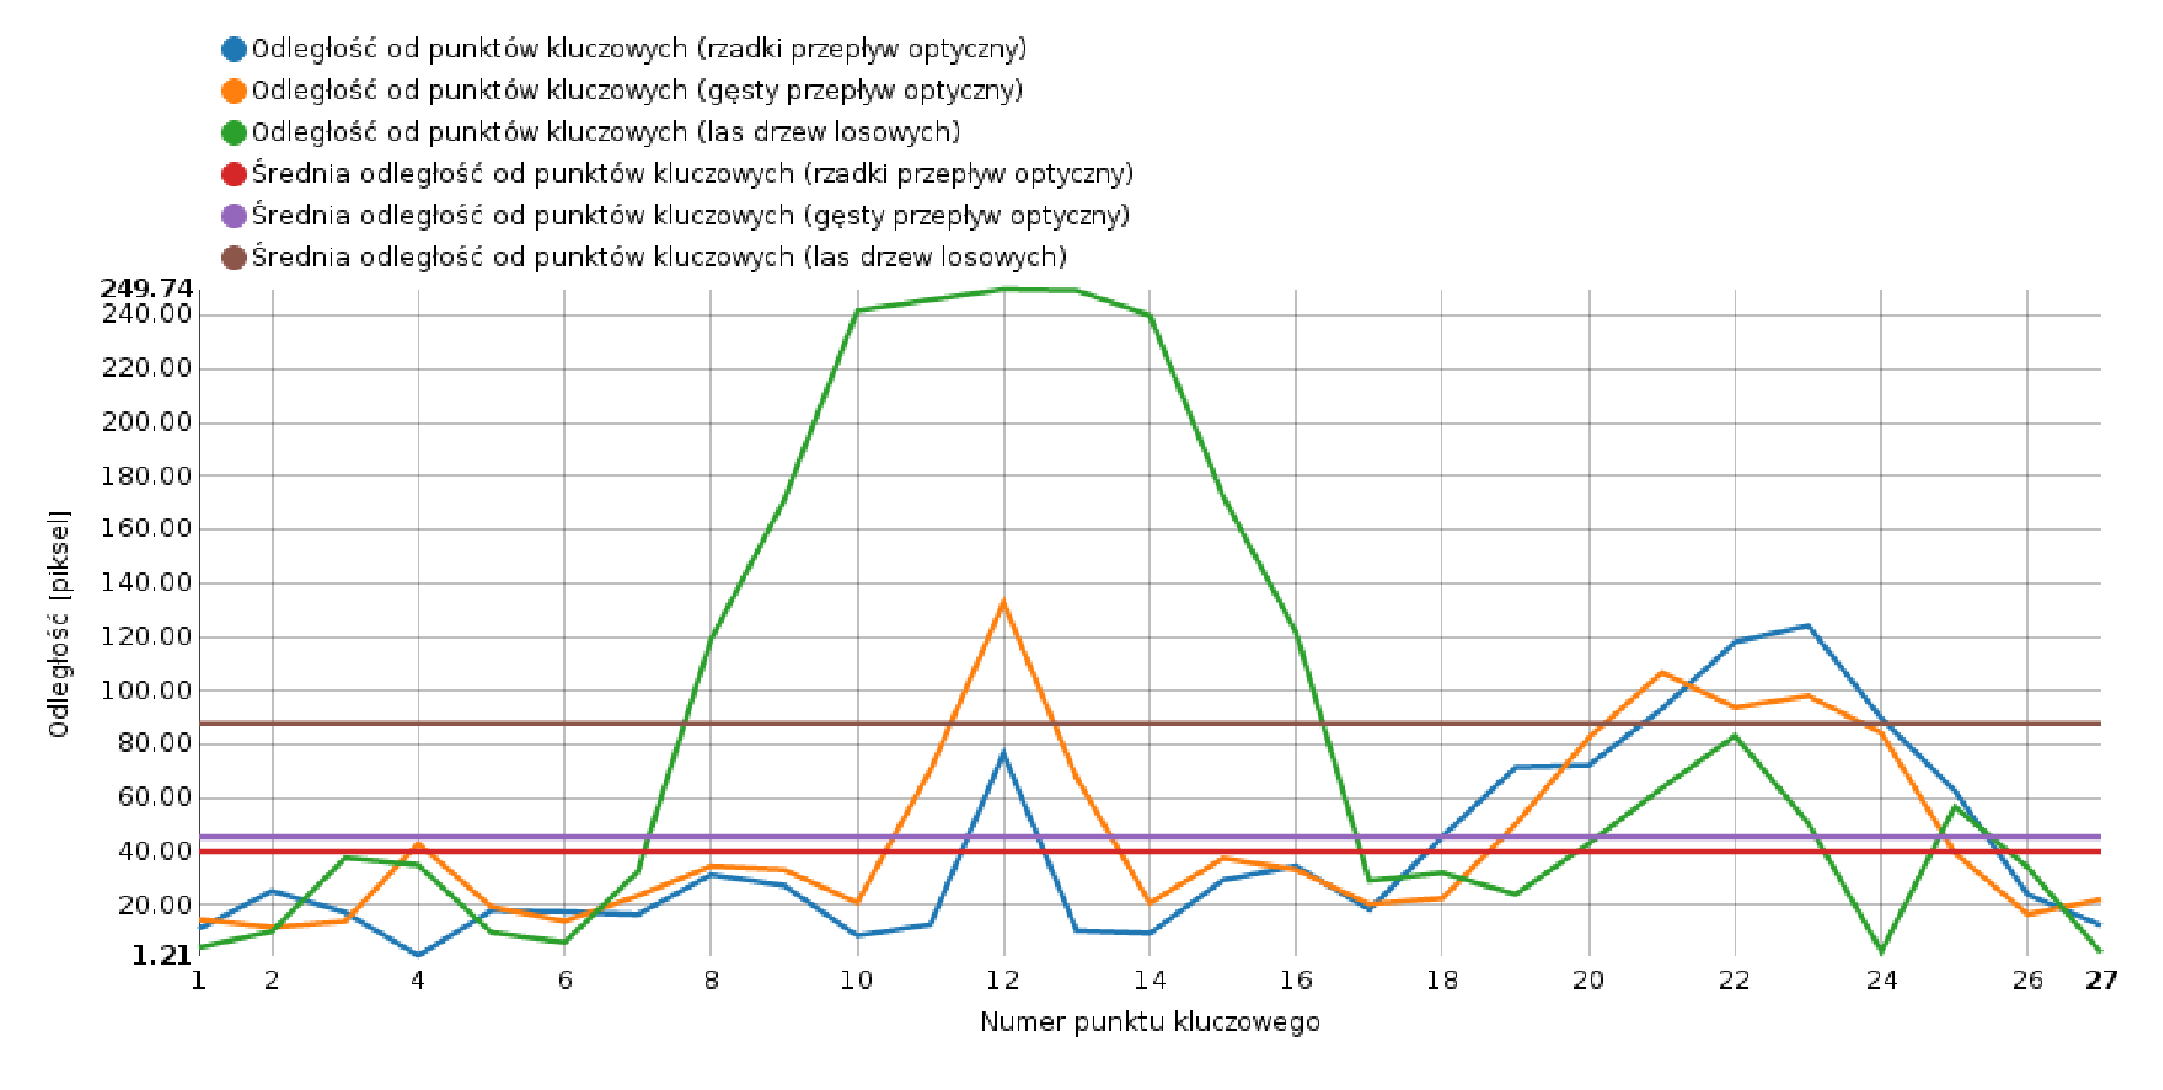
\includegraphics[width=14cm]{charts/quality/KeypointsQualityAC}
        \caption[Odległość od punktów wzorcowych (próbka osoby A, gest C)]
                {Odległość od punktów wzorcowych dla próbki \textit{Person\_A\_C}}
        \label{fig:KeypointsQualityAC}
      \end{figure}

      \begin{figure}[!ht]
        \centering
        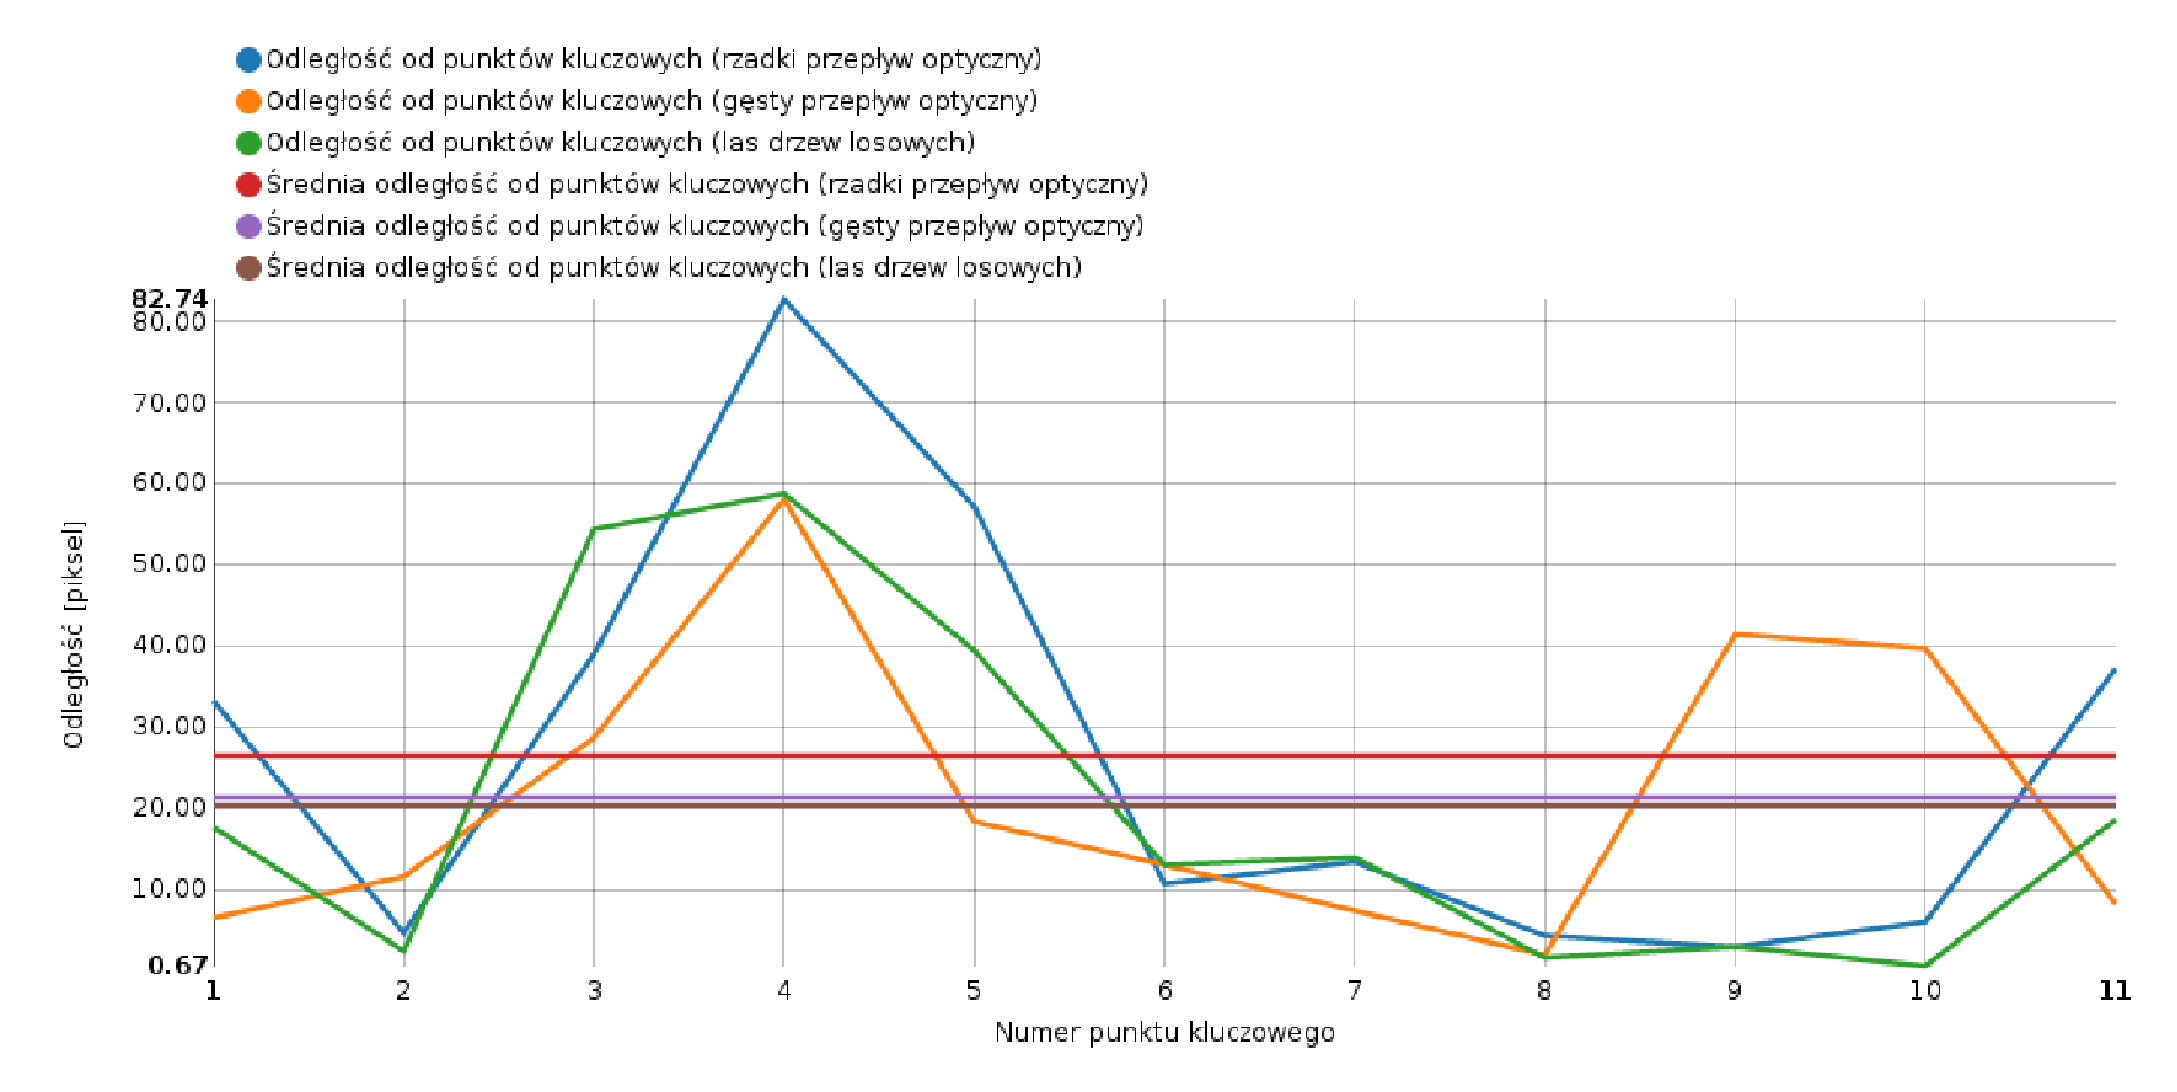
\includegraphics[width=14cm]{charts/quality/KeypointsQualityGO}
        \caption[Odległość od punktów wzorcowych (próbka osoby G, gest O)]
                {Odległość od punktów wzorcowych dla próbki \textit{Person\_G\_O}}
        \label{fig:KeypointsQualityGO}
      \end{figure}

    Poniżej można zaobserwować po raz kolejny jest problem niestabilności metody opartej o~proces uczenia maszynowego (środkowa część wykresu \ref{fig:PathQualityAC}). W~przypadku próbek \textit{Person\_A\_C} oraz \textit{Person\_G\_O} najmniejszy błąd jeśli chodzi o~odległość od ścieżek wzorcowych został zaprezentowany przez algorytm przepływu optycznego w~wariancie gęstym. Metoda oparta o~algorytm \textit{LK} dla analizowanych próbek była nieznacznie gorsza od najlepszej implementacji.

    \newpage
      \begin{figure}[!ht]
        \centering
        \includegraphics[width=14cm]{charts/quality/PathQualityAC}
        \caption[Odległość od ścieżek wzorcowych (próbka osoby A, gest C)]
                {Odległość od ścieżek wzorcowych dla próbki \textit{Person\_A\_C}}
        \label{fig:PathQualityAC}
      \end{figure}

      \begin{figure}[!ht]
        \centering
        \includegraphics[width=14cm]{charts/quality/PathQualityGO}
        \caption[Odległość od ścieżek wzorcowych (próbka osoby G, gest O)]
                {Odległość od ścieżek wzorcowych dla próbki \textit{Person\_G\_O}}
        \label{fig:PathQualityGO}
      \end{figure}

    Ciekawym przypadkiem jest próbka \textit{Person\_G\_C}, w~której stabilnie zaprezentował się algorytm wykorzystujący las drzew losowych. Rezultat obliczony za pomocą tej metody charakteryzował się najmniejszym błędem i~najlepszą jakością, co zostało zobrazowane na wykresach \ref{fig:DenseQualityKeypointsGC}, \ref{fig:RandomQualityKeypointsGC} oraz \ref{fig:SparseQualityKeypointsGC} (oraz \ref{fig:DenseQualityPathGC}, \ref{fig:RandomQualityPathGC}, \ref{fig:SparseQualityPathGC}). Rezultat ten pozwala wierzyć, że po wprowadzeniu usprawnień do procesu budowy bazy treningowej i~dopracowaniu samego klasyfikatora (poprzez uodpornienie na sytuacje brzegowe tj. zmiana kształtu dłoni) algorytm ten będzie najdokładniejszy.

    \newpage
      \begin{figure}[!ht]
        \centering
        \includegraphics[width=10cm]{charts/quality/DenseQualityKeypointsGC}
        \caption[Odległość od punktów wzorcowych dla jednego algorytmu (gęsty przepływ optyczny, osoba G, gest C)]
                {Odległość od punktów wzorcowych dla jednego algorytmu\\(gęsty przepływ optyczny, próbka \textit{Person\_G\_C})}
        \label{fig:DenseQualityKeypointsGC}
      \end{figure}

      \begin{figure}[!ht]
        \centering
        \includegraphics[width=10cm]{charts/quality/RandomQualityKeypointsGC}
        \caption[Odległość od punktów wzorcowych dla jednego algorytmu (las drzew losowych, osoba G, gest C)]
                {Odległość od punktów wzorcowych dla jednego algorytmu\\
                 (las drzew losowych, próbka \textit{Person\_G\_C})}
        \label{fig:RandomQualityKeypointsGC}
      \end{figure}

      \begin{figure}[!ht]
        \centering
        \includegraphics[width=10cm]{charts/quality/SparseQualityKeypointsGC}
        \caption[Odległość od punktów wzorcowych dla jednego algorytmu (rzadki przepływ optyczny, osoba G, gest C)]
                {Odległość od punktów wzorcowych dla jednego algorytmu\\(rzadki przepływ optyczny, próbka \textit{Person\_G\_C})}
        \label{fig:SparseQualityKeypointsGC}
      \end{figure}

    \newpage
      \begin{figure}[!ht]
        \centering
        \includegraphics[width=10cm]{charts/quality/DenseQualityPathGC}
        \caption[Odległość od ścieżek wzorcowych dla jednego algorytmu  (gęsty przepływ optyczny, osoba G, gest C)]
                {Odległość od ścieżek wzorcowych dla jednego algorytmu\\(gęsty przepływ optyczny, próbka \textit{Person\_G\_C})}
        \label{fig:DenseQualityPathGC}
      \end{figure}

      \begin{figure}[!ht]
        \centering
        \includegraphics[width=10cm]{charts/quality/RandomQualityPathGC}
        \caption[Odległość od ścieżek wzorcowych dla jednego algorytmu (las drzew losowych, osoba G, gest C)]
                {Odległość od ścieżek wzorcowych dla jednego algorytmu\\
                 (las drzew losowych, próbka \textit{Person\_G\_C})}
        \label{fig:RandomQualityPathGC}
      \end{figure}

      \begin{figure}[!ht]
        \centering
        \includegraphics[width=10cm]{charts/quality/SparseQualityPathGC}
        \caption[Odległość od ścieżek wzorcowych dla jednego algorytmu (rzadki przepływ optyczny, osoba G, gest C)]
                {Odległość od ścieżek wzorcowych dla jednego algorytmu\\(rzadki przepływ optyczny, próbka \textit{Person\_G\_C})}
        \label{fig:SparseQualityPathGC}
      \end{figure}

    \newpage
      \begin{figure}[!ht]
        \centering
        \includegraphics[width=10cm]{charts/quality/DenseScatterGC}
        \caption[Wykres rozproszenia punktów (gęsty przepływ optyczny)]
                {Wykres rozproszenia punktów\\(gęsty przepływ optyczny, próbka \textit{Person\_G\_C})}
        \label{fig:DenseScatterGC}
      \end{figure}

      \begin{figure}[!ht]
        \centering
        \includegraphics[width=10cm]{charts/quality/RandomScatterGC}
        \caption[Wykres rozproszenia punktów (las drzew losowych)]
                {Wykres rozproszenia punktów\\(las drzew losowych, próbka \textit{Person\_G\_C})}
        \label{fig:RandomScatterGC}
      \end{figure}

      \begin{figure}[!ht]
        \centering
        \includegraphics[width=10cm]{charts/quality/SparseScatterGC}
        \caption[Wykres rozproszenia punktów (rzadki przepływ optyczny)]
                {Wykres rozproszenia punktów\\(rzadki przepływ optyczny, próbka \textit{Person\_G\_C})}
        \label{fig:SparseScatterGC}
      \end{figure}

    Na wykresach \ref{fig:DenseScatterGC}, \ref{fig:RandomScatterGC}, \ref{fig:SparseScatterGC} została przedstawiona wizualna reprezentacja wyznaczonych punktów charakterystycznych wyznaczonej ścieżki (kolor zielony) oraz najbliższych uśrednionych punktów (kolor niebieski) w~odniesieniu do wyznaczonych manualnie punktów wzorcowych (kolor czerwony). Promień okręgu otaczającego punkt wzorcowy jest wprost proporcjonalny do błędu (odległości najbliższego średniego punktu). Po analizie wzrokowej, widać że największe czerwone punkty (zwłaszcza na boku wyznaczonego kształtu) posiada metoda wykorzystująca las drzew losowych.

      \begin{figure}[!ht]
        \centering
        \includegraphics[width=14cm]{charts/quality/DenseKeypointsPerMapSize}
        \caption[Odległości od punktów wzorcowych w~zależności od rozmiaru siatki]
                {Odległości od punktów wzorcowych w~zależności od rozmiaru siatki (gęsty przepływ optyczny)}
        \label{fig:DenseKeypointsPerMapSize}
      \end{figure}

      \begin{figure}[!ht]
        \centering
        \includegraphics[width=14cm]{charts/quality/DensePathPerMapSize}
        \caption[Odległość od ścieżek wzorcowych w~zależności od rozmiaru siatki]
                {Odległość od ścieżek wzorcowych w~zależności od rozmiaru siatki (gęsty przepływ optyczny)}
        \label{fig:DensePathPerMapSize}
      \end{figure}

    W~przypadku wykresów \ref{fig:DenseKeypointsPerMapSize} oraz \ref{fig:DensePathPerMapSize} zaprezentowany został spadek jakości wraz ze~zwiększającym się rozmiarem siatki dla przepływu optycznego w~wariancie gęstym.

    \newpage
      \begin{figure}[!ht]
        \centering
        \includegraphics[width=14cm]{charts/quality/RandomKeypointsPerTrainedTreesAmount}
        \caption[Odległości od punktów wzorcowych w~zależności od liczby drzew losowych]
                {Odległości od punktów wzorcowych w~zależności od liczby drzew losowych (las drzew losowych)}
        \label{fig:RandomKeypointsPerTrainedTreesAmount}
      \end{figure}

      \begin{figure}[!ht]
        \centering
        \includegraphics[width=14cm]{charts/quality/RandomPathPerTrainedTreesAmount}
        \caption[Odległości od ścieżek wzorcowych w~zależności od liczby drzew losowych]
                {Odległości od ścieżek wzorcowych w~zależności od liczby drzew losowych (las drzew losowych)}
        \label{fig:RandomPathPerTrainedTreesAmount}
      \end{figure}

    Dla metody lasów losowych liczba drzew losowych wpływa w~niewielkim stopniu na jakość, co zostało zaprezentowane na wykresach \ref{fig:RandomKeypointsPerTrainedTreesAmount} oraz \ref{fig:RandomPathPerTrainedTreesAmount}. Większa wartość omawianego współczynnika pozwala w~niewielkim stopniu zmniejszyć maksymalny błąd (wartości od 30 do 45) związany z~odległością od punktów wzorcowych.

    \newpage
      \begin{figure}[!ht]
        \centering
        \includegraphics[width=14cm]{charts/quality/KeypointsDistanceSparsePerMinimalDistance}
        \caption[Odległość od punktu wzorcowego w~zależności od minimalnej odległości pomiędzy punktami
                 charakterystycznymi]
                {Odległość od punktu wzorcowego w~zależności od minimalnej odległości pomiędzy punktami
                 charakterystycznymi (rzadki przepływ optyczny)}
        \label{fig:SpecialisedSparseKeypointsDistance}
      \end{figure}

      \begin{figure}[!ht]
        \centering
        \includegraphics[width=14cm]{charts/quality/PathDistanceSparsePerMinimalDistance}
        \caption[Odległość od ścieżki wzorcowej w~zależności od minimalnej odległości pomiędzy punktami
                 charakterystycznymi]
                {Odległość od ścieżki wzorcowej w~zależności od minimalnej odległości pomiędzy punktami
                 charakterystycznymi (rzadki przepływ optyczny)}
        \label{fig:SpecialisedSparsePathDistance}
      \end{figure}

    Jak wspomniano w~sekcji \ref{Section_Overhead} i~co widać na wykresach \ref{fig:SpecialisedSparseKeypointsDistance} oraz \ref{fig:SpecialisedSparsePathDistance}, warto zwiększyć wartość współczynnika minimalnej odległości pomiędzy punktami charakterystycznymi, w~celu zmniejszenia maksymalnego błędu (odległości od ścieżek oraz punktów wzorcowych). Dzięki temu zmniejszy się również, wartość średnia odległości i~poprawi jakość ścieżki wyznaczonej ze śledzonych punktów.

\chapter{Usprawnienia i~podsumowanie}\label{Chapter_Podsumowanie}

  \section{Proponowane usprawnienia}\label{Section_Usprawnienia}

    Na podstawie analizy zawartej w~powyższych podrozdziałach nasuwa się kilka wniosków i~potencjalnych ulepszeń. Zostały one zebrane i~omówione poniżej.

    \begin{itemize}
      \item \textbf{Rozszerzenie sposobu budowania bazy treningowej dla algorytmu wykorzystującego las drzew losowych.}

      Aby zwiększyć jakość klasyfikacji oraz jeszcze bardziej uodpornić algorytm na zmianę kształtu śledzonej dłoni należy udoskonalić proces generacji danych wejściowych. Potencjalnym rozszerzeniem może być wykorzystanie nie tylko pierwszej klatki animacji, do generowania zbioru danych treningowych. Innym rozszerzeniem, może być dodanie kolejnych transformacji źródłowej klatki animacji (np. celowego zniekształcenia perspektywy lub tzw. \textit{rybiego oka} oraz dodatkowego rodzaju szumu).

      \item \textbf{Optymalizacja zużycia pamięci dla algorytmu przepływu optycznego gęstego.}

      W~sekcji \ref{Section_Memory} podczas omawiania zużycia pamięci dla wspomnianego algorytmu dało się zauważyć ciągłą zmianę zużywanej pamięci fizycznej (i~w konsekwencji także wirtualnej, rysunek \ref{fig:OpticalFlowsMemoryUsage}). Ciągła alokacja i~zwalnianie przydzielonych zasobów negatywnie wpływa na czas przetwarzania klatki sekwencji wideo. Narzut ten, może zostać zniwelowany za pomocą zmiany sposobu alokacji pamięci np. poprzez zastosowanie wielokrotnie wykorzystywanej i~współdzielonej puli pamięci.

      \item \textbf{Optymalizacja zużycia pamięci dla algorytmu opartego o drzewa losowe.}

      Omawiany algorytm podczas pracy wykorzystuje bardzo dużo (w~odniesieniu do pozostałych dwóch metod) pamięci fizycznej. W~celu zwiększenia przydatności algorytmu należy przeprowadzić proces optymalizacji zużycia pamięci.

      \item \textbf{Przyspieszenie procesu uczenia, odczytu oraz zapisu bazy treningowej.}

       W~obecnej implementacji przy generacji, zapisie oraz odczycie bazy treningowej wykorzystywany jest jeden wątek (w~konsekwencji również jeden procesor). W~oryginalnym algorytmie (opisanym w~pracy \cite{RandomizedTrees06}) autorzy proponują rozdzielenie omawianych etapów pracy algorytmu na cztery wątki, co zdecydowanie lepiej wykorzystuje możliwości współczesnego sprzętu.
    \end{itemize}

  \section{Podsumowanie}

    W~ramach pracy magisterskiej omówiono i~przeprowadzono badania wydajnościowe oraz jakościowe implementacji trzech algorytmów śledzenia punktów charakterystycznych pod kątem wykorzystania ich do analizy ruchu dłoni.

    Zebrane rezultaty pozwoliły na jednoznaczne określenie przydatności poszczególnych algorytmów w~badanym obszarze. Dokładne wnioski oraz~decyzje zostały zebrane i~opisane w~poprzednim rozdziale.

    Oprócz zaproponowanych implementacji, badań oraz~analizy zostały również zaproponowane usprawnienia i~potencjalne rozszerzenia, które zwiększą jakość oraz poprawia wydajność omawianych metod.